\documentclass[11pt,english,italian,openright]{book}
\usepackage[ansinew]{inputenc}
\usepackage[a4paper]{geometry}
\geometry{verbose,tmargin=3cm,bmargin=3.5cm,lmargin=4cm,rmargin=3cm}
\setcounter{secnumdepth}{3}
\setcounter{tocdepth}{3}
\usepackage{color}
\usepackage[italian]{babel}
\usepackage{float}
\usepackage{booktabs}
\usepackage{url}
\usepackage{amsmath}
\usepackage{amssymb}
\usepackage{graphicx}
\usepackage{setspace}
\usepackage{esint}
\onehalfspacing
\usepackage[unicode=true,pdfusetitle,
 bookmarks=true,bookmarksnumbered=false,bookmarksopen=false,
 breaklinks=false,pdfborder={0 0 0},backref=false,colorlinks=false]
 {hyperref}

\makeatletter

%% Because html converters don't know tabularnewline
\providecommand{\tabularnewline}{\\}
\floatstyle{ruled}
\newfloat{algorithm}{tbp}{loa}[chapter]
\providecommand{\algorithmname}{Algoritmo}
\floatname{algorithm}{\protect\algorithmname}

%%%%%%%%%%%%%%%%%%%%%%%%%%%%%% User specified LaTeX commands.
% pacchetti aggiuntivi
\usepackage{tabularx}
\usepackage{setspace}
\usepackage{amsthm}
\usepackage{rotating}
\usepackage{caption}
\usepackage{epsfig}
\usepackage{indentfirst}
\usepackage{fancyhdr}
\usepackage{url}
\usepackage{cite}
\usepackage[normalem]{ulem}
\usepackage[table]{xcolor}
\usepackage{booktabs}
\usepackage{algpseudocode}

% sistema il numero pagina nelle prime pagine dei capitoli
\fancypagestyle{plain}{
\fancyhead{}
\renewcommand{\headrulewidth}{0pt}
\renewcommand{\footrulewidth}{0pt}
\fancyfoot[OC]{\begin{flushright}\thepage\end{flushright}}
}

% header "carini" per la tesi
\fancyhead{}
\fancyhead[LE]{\slshape \nouppercase \leftmark}
\fancyhead[RO]{\slshape \nouppercase \rightmark}
\fancyfoot[EC]{\begin{flushleft}\thepage\end{flushleft}}
\fancyfoot[OC]{\begin{flushright}\thepage\end{flushright}}
\renewcommand{\headrulewidth}{0.4pt}
\setlength{\headheight}{14pt}

\@ifundefined{showcaptionsetup}{}{%
 \PassOptionsToPackage{caption=false}{subfig}}
\usepackage{subfig}
\makeatother

\usepackage{listings}
\addto\captionsenglish{\renewcommand{\algorithmname}{Algorithm}}
\addto\captionsenglish{\renewcommand{\lstlistingname}{Listing}}
\addto\captionsitalian{\renewcommand{\algorithmname}{Algoritmo}}
\addto\captionsitalian{\renewcommand{\lstlistingname}{Listato}}
\renewcommand{\lstlistingname}{Listato}

%comandi personalizzati
\newcommand{\virgolette}[1]{``#1''}
\newcommand{\upe}{\`E }

\begin{document}
\frontmatter
\pagestyle{empty}
\newgeometry{margin=3cm}\begin{titlepage}

\begin{center}
\Large{\textsc{Politecnico di Milano}}\\
\Large{Scuola di Ingegneria Industriale e dell'Informazione}\\
\large{Corso di Laurea Magistrale in Ingegneria Informatica}\\
\large{Dipartimento di Elettronica, Informazione e Bioingegneria}
\par\end{center}

\vspace{0.5cm}


\begin{center}
\begin{figure}[h]
\centering{}
\includegraphics[width=0.5\textwidth]{frontespizio/logo-polimi.png}
\end{figure}
\vspace{1cm}

\par\end{center}

\begin{center}
\LARGE{Progettazione dei mashup per dispositivi mobili: un metodo basato sulla modellazione del contesto}\vspace{2cm}

\par\end{center}

\begin{flushleft}
\begin{tabular}{ll}
Relatore:  & Prof.ssa Letizia TANCA\tabularnewline
Correlatori:  & Prof.ssa Maristella MATERA\tabularnewline
	& Prof. Vittorio ZACCARIA
\end{tabular}\vspace{1cm}

\par\end{flushleft}

\begin{flushright}
\begin{tabular}{ll}
Tesi di laurea di: & \tabularnewline
Valerio CASSANI & Matr. 817398\tabularnewline
Stefano GIANELLI & Matr. 817014\tabularnewline
\end{tabular}\vspace{2.2cm}

\par\end{flushright}

\begin{center}
{\large{}Anno Accademico 2014\textendash 2015}
\par\end{center}{\large \par}

\end{titlepage}
\restoregeometry

\cleardoublepage{}

%\begin{flushright}
%\emph{Ad una persona veramente speciale\ldots{}
}\cleardoublepage{}
%\par\end{flushright}


\chapter*{Ringraziamenti}

\thispagestyle{empty}Vorrei cominciare questa pagina di ringraziamenti con le persone che hanno collaborato a questo progetto.
Un grazie a Letizia e Maristella, che ci hanno sempre seguito in questi mesi in questo lavoro, sostenendoci e aiutandoci in particolare nella parte metodologica. Grazie a Vittorio e Riccardo che ci hanno aiutato nella parte tecnica, facendomi scoprire nuove tecnologie e metodi.
Un ringraziamento particolare va a Stefano che ho conosciuto quando sono entrato in questo team ed è stato un piacere lavorare con lui e penso di aver imparato moltissimo. 
Poi vorrei ringraziare tutte le persone che ho incontrato qui al Politecnico, penso che ognuno mi abbia trasmesso un insegnamento, un modo di lavorare e ho conosciuto dei veri amici disponibili in tutto e per tutto, anche per studiare insieme per gli esami e svolgere i progetti.
Vorrei ringraziare la mia famiglia: i miei genitori, che mi hanno sostenuto anche in questi anni di università, i miei due fratelli, i nonni, zii e tutti gli altri parenti che mi hanno trasmesso una serie di valori che mi porterò per tutta la vita. 

Un grazie particolare va a Rebecca che mi ha sopportato anche nel periodo da tesista, non facendo mai mancare il suo aiuto per qualsiasi cosa avessi bisogno. (PS: prima o poi informatica te la farò passare!)

Per ultimi ma non per importanza vorrei ringraziare la mia compagnia di amici, che sono sempre presenti se era necessario qualche consiglio e per tutte le serate e i momenti che abbiamo trascorso insieme.

\vspace{1cm}

\begin{flushright}
	Valerio
\end{flushright}


\clearpage

Il mio primo ringraziamento va a tutto il gruppo di lavoro che mi ha accolto con tanto affetto e mi ha accompagnato durante tutto il lavoro. Ringrazio Letizia e Maristella per avermi dato la possibilità di lavorare su questo progetto e per essere state sempre disponibili e di estremo aiuto. Ringrazio Vittorio e Riccardo per i preziosi consigli e per avermi spronato a fare sempre di meglio. 

Ringrazio i miei genitori, senza i quali non avrei mai potuto completare questo percorso.

Ringrazio anche il mio fidato compagno di tesi Valerio, capitato per caso ma col quale è stato veramente un piacere condividere questa esperienza. Se questa tesi sarà un successo è anche merito tuo!

Più di un ringraziamento è d’obbligo ad Alessandro, Andrea e Francesca che mi hanno accompagnato in questa avventura. Senza il vostro supporto non sarei mai arrivato a questo giorno! In realtà Andrea dovrei ringraziarti più per le abbuffate, i caffè e i viaggi folli di questi anni.

Devo più di un ringraziamento a Sara. Ci siamo incontrati tardi ma in te ho trovato una vera amica. Le giornate passate assieme al Poli mi mancano molto!

Devo ringraziare il mio fidato amico Andrea, col quale condivido ormai da una vita qualsiasi cosa. Probabilmente non te lo dico spesso ma la tua amicizia significa molto per me, avere il tuo supporto mi ha aiutato molto in questi anni.

Ringrazio Lorenzo, Giacomo, Lorenzo, Nicolò, Elisa, Wanda e Mara, fidati compagni di uscite e vacanze. Con alcuni di voi è stato anche un immenso piacere condividere i meravigliosi anni delle scuole superiori. Sono felice di aver conosciuto ognuno di voi e di aver condiviso tantissime meravigliose esperienze.

Ringrazio Nelya, per aver sopportato tutte le mie lamentele (e io le tue). Hai sempre saputo esattamente cosa dire nei momenti più difficili ma è stato sempre un piacere parlare con te, in qualsiasi situazione, mi sei stata di grandissimo aiuto.

\vspace{1cm}

\begin{flushright}
	Stefano
\end{flushright}\cleardoublepage{}


\chapter*{Sommario}

\thispagestyle{empty}Data la sovrabbondanza di dati e servizi disponibili online è spesso difficile trovare informazioni e applicazioni adatte al contesto corrente. Questa situazione è accentuata se la ricerca di dati è eseguita su dispositivi mobili, dove le risorse (memoria, capacità computazionale, piano dati modesto) sono limitate.

Date queste premesse questa tesi mira alla definizione di metodologie e strumenti per la progettazione e sviluppo di \emph{Context-Aware Mobile mashUpS} (\emph{CAMUS}). Le applicazioni \emph{CAMUS} recuperano e integrano i dati dinamicamente da risorse online (interrogate tramite web \emph{API}) e si occupano di ritagliare le informazioni acquisite in base alla situazione nella quale si trova l'utente. Offrono numerosi vantaggi grazie alla capacità di identificare fonti pertinenti, selezionate in base alla loro adeguatezza rispetto alle esigenze dell'utente, i cui dati sono integrati e forniti sotto forma di \emph{mobile app}.

Questo paradigma permette di superare i limiti delle applicazioni preconfezionate e mette a disposizione applicazioni flessibili e personalizzate la cui struttura e contenuti possono variare in fase di esecuzione in base alla situazione d'uso. Un esempio di beneficio è l'integrazione dei contenuti principali con servizi di supporto, come le mappe, le informazioni sul meteo o il trasporto pubblico, che possono migliorare l'esperienza d'uso.

Questa tesi presenta una metodologia di progettazione e una piattaforma per la creazione di applicazioni CAMUS. L'approccio \emph{i)} utilizza la modellazione del contesto come strumento principale per individuare le risorse più adatte per soddisfare i bisogni dell'utente e \emph{ii)} individua in fase di esecuzione come ritagliare i dati e le funzioni recuperate dalle risorse selezionate. L'astrazione fornita dal contesto, infatti, viene utilizzata per generare modelli che definiscono come i dati recuperati andranno integrati e visualizzati. Questi modelli definiscono le regole di esecuzione dinamica delle \emph{mobile app}. La tesi inoltre descrive un prototipo che fa uso delle tecnologie \emph{web} e \emph{mobile} più recenti per supportare la modellazione delle applicazioni CAMUS, la generazione automatica del codice e l'esecuzione delle applicazioni finali.\cleardoublepage{}


\chapter*{Abstract}

\thispagestyle{empty}\selectlanguage{english}%
\selectlanguage{italian}%

\cleardoublepage{}\pagenumbering{roman}
\setcounter{page}{1}
\pagestyle{fancy}\tableofcontents{}\listoffigures
\listoftables
\listof{algorithm}{Elenco degli algoritmi}
\cleardoublepage{}\mainmatter
\renewcommand{\sectionmark}[1]{\markright{\thesection.\ #1}}
\renewcommand{\chaptermark}[1]{\markboth{\thechapter.\ #1}{}}


\chapter{Introduzione\label{ch:introduzione}}

Negli ultimi anni si è assistito a un'enorme diffusione di Internet e soprattutto di una varietà di dispositivi con i quali è possibile accedervi: mentre agli albori esistevano solamente PC desktop, con i quali poter visitare pagine per lo più statiche, al giorno d'oggi sono disponibili dispositivi come smartphone e tablet che ci permettono di rimanere sempre connessi. Grazie al fatto di essere estremamente portatili e semplici da utilizzare essi sono ormai diventati oggetti indispensabili nella vita quotidiana. Lo scorso anno è avvenuto il sorpasso della quantità di traffico generata da smartphone e tablet rispetto ai PC (Figura \ref{fig:traffico-tipologia-dispositivo}). L'incremento della velocità delle connessioni e il progresso tecnologico ha fatto sì che sia possibile consultare qualsiasi tipo di informazione su internet, dal semplice testo fino a immagini, video, ecc.

\begin{figure}[ht]
	\centering
	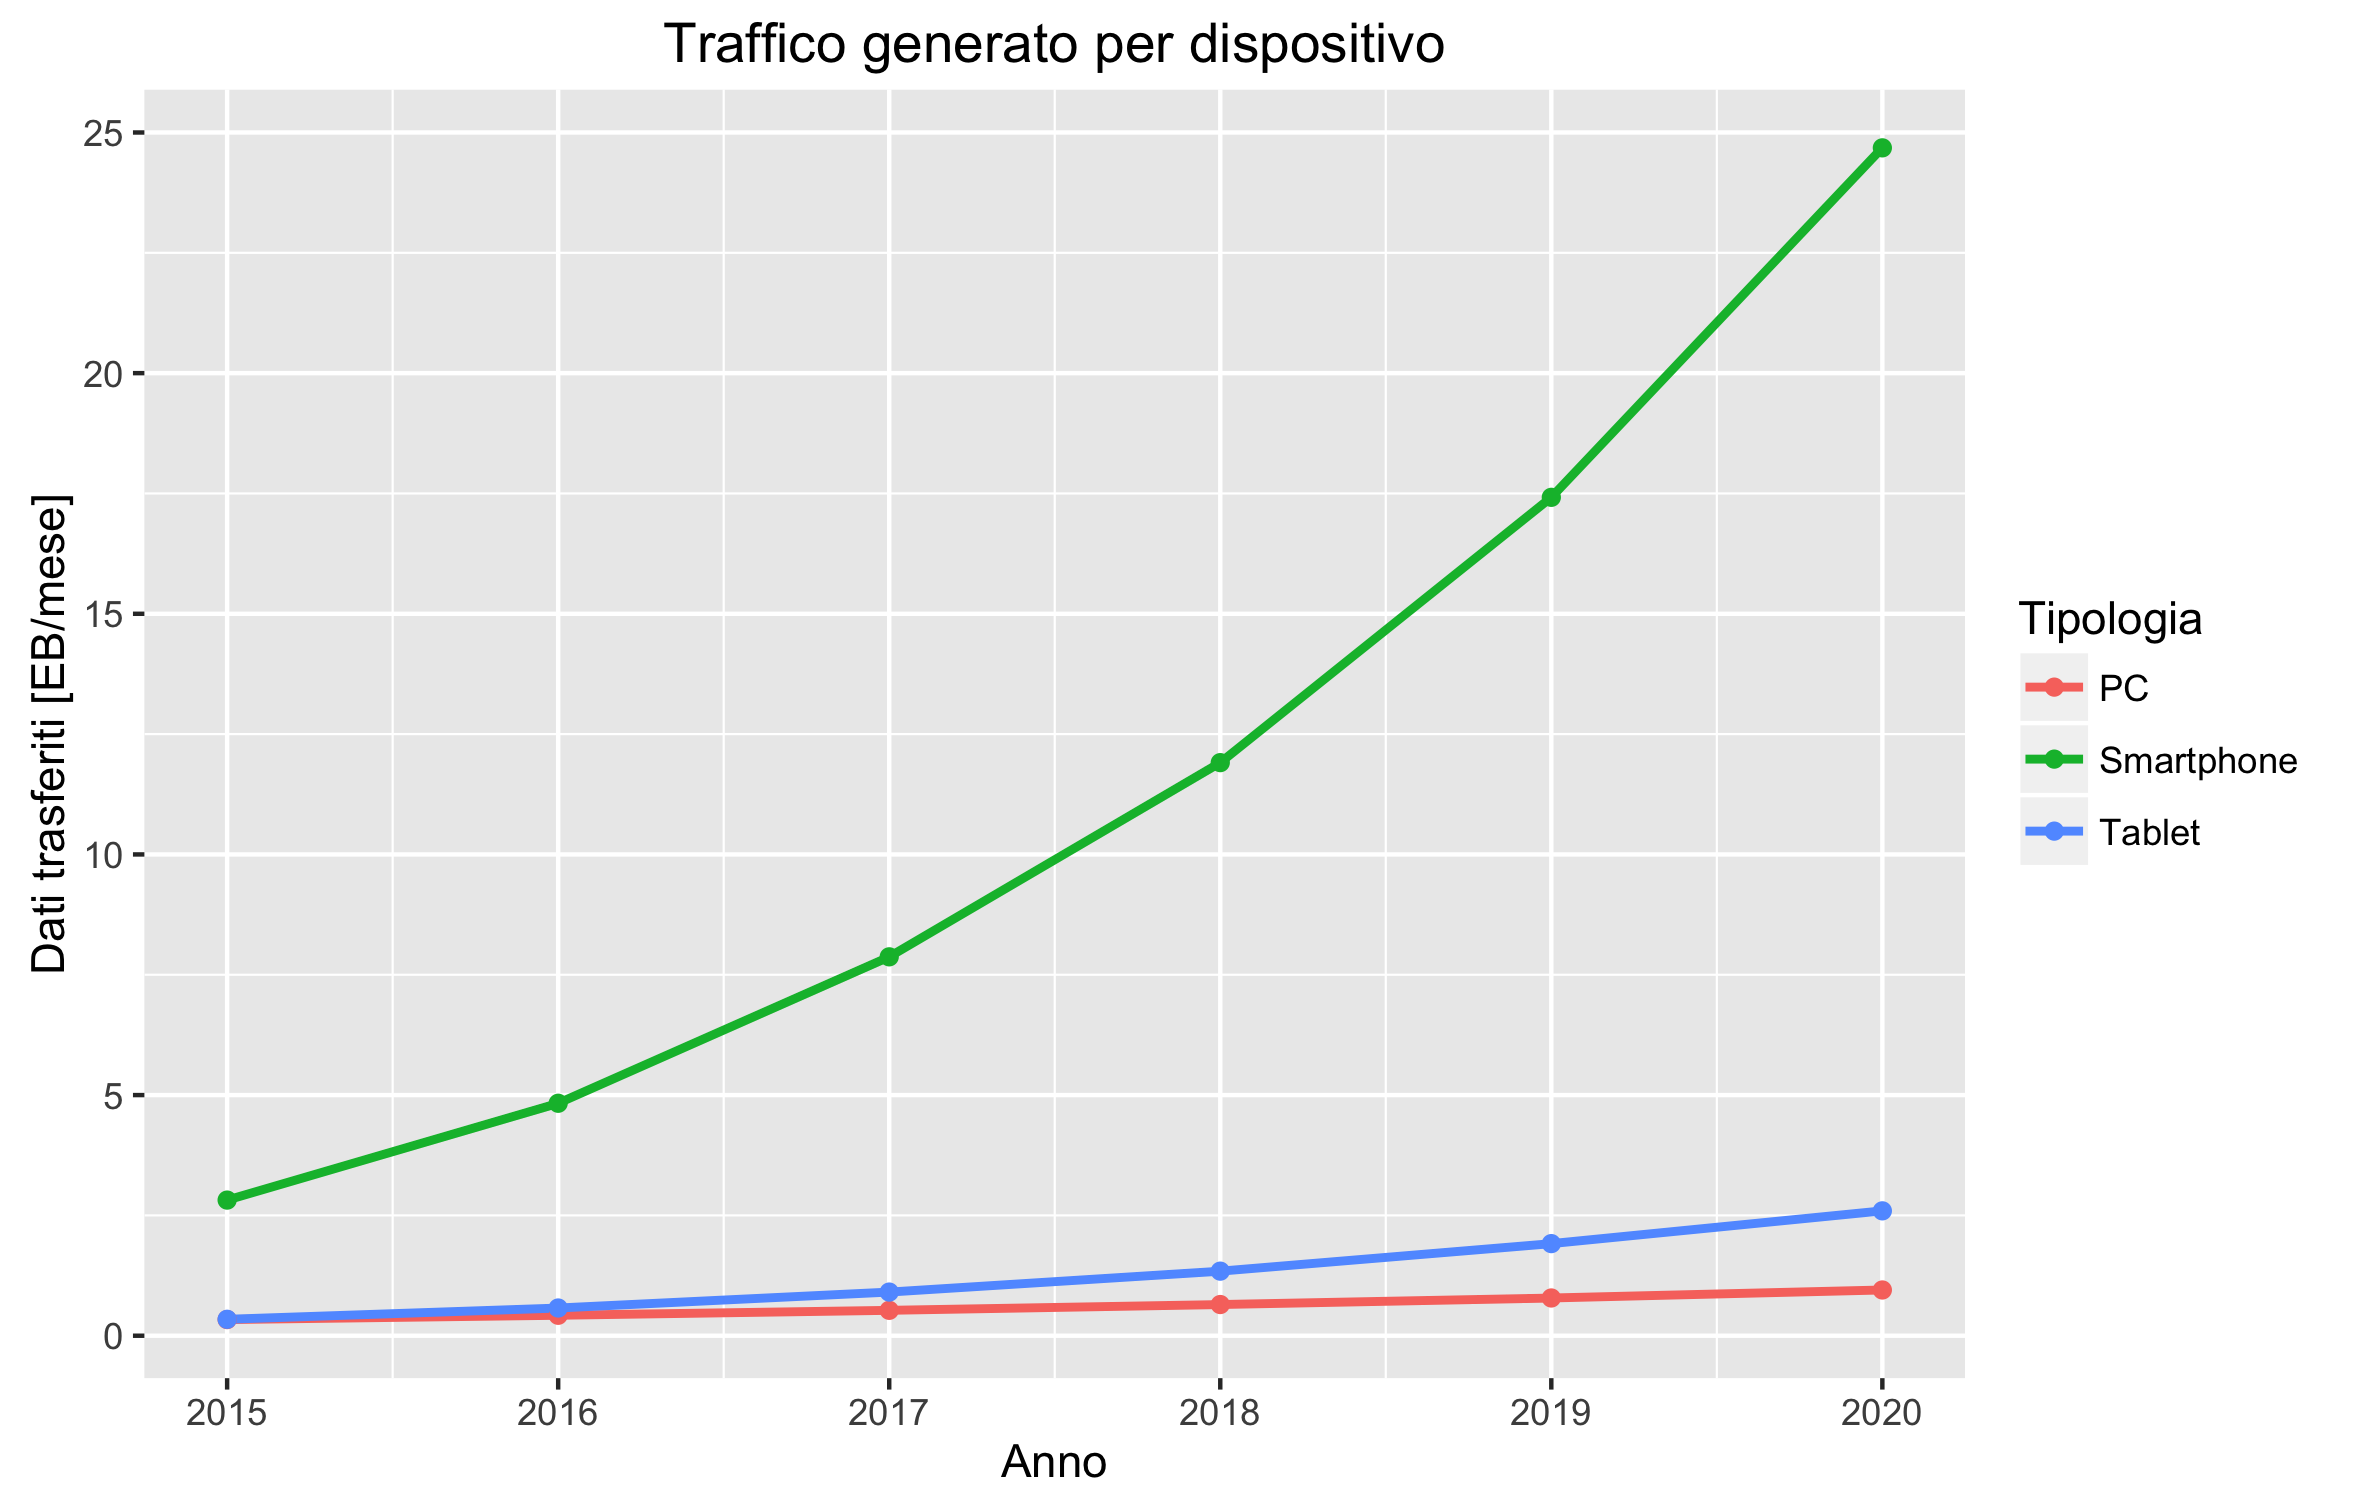
\includegraphics[width=\textwidth]{1-introduzione/Immagini/traffico-dispositivi.png}
	\caption[Traffico generato per tipologia di dispositivo]{Traffico generato per tipologia di dispositivo (fonte: Cisco, 2016)\label{fig:traffico-tipologia-dispositivo}}
\end{figure}

Si è persa anche la tradizione che sia un gestore a pubblicare contenuti in quanto ormai sono direttamente gli utenti a produrre la maggior parte delle informazioni disponibili (Figura \ref{fig:analisi-dati-generati}). Questo fenomeno è stato accentuato con la creazione dei \emph{social network}, che permettono di creare collegamenti tra le persone e dove è possibile condividere qualunque cosa che ognuno trova interessante. Gli utenti vengono così coinvolti nella creazione di contenuti di varia natura. Per esempio possono essere anche di tipo multimediale, grazie alla dotazione di fotocamera ad alta risoluzione nei dispositivi.

\begin{figure}[ht]
	\centering
	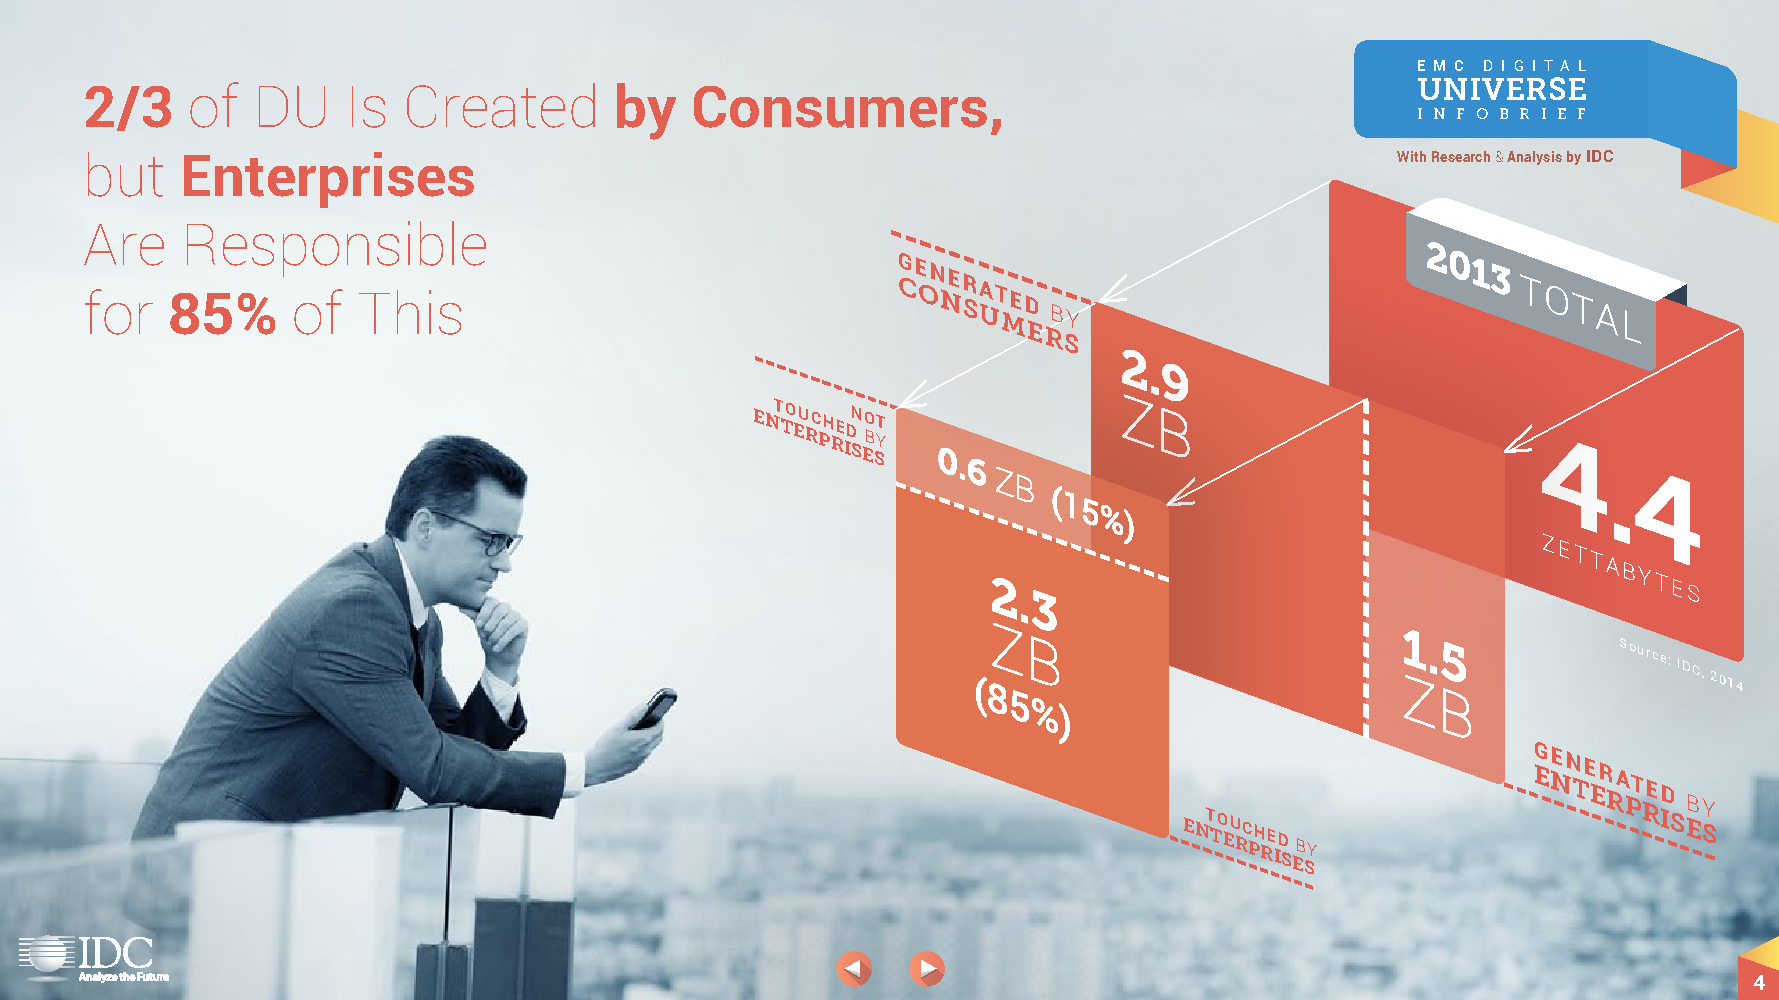
\includegraphics[width=\textwidth]{1-introduzione/Immagini/dati-generati-consumer.pdf}
	\caption[Analisi della quantità di dati generati]{Analisi della quantità di dati generati (fonte: IDC, 2014)\label{fig:analisi-dati-generati}}
\end{figure}

Come si può notare in Figura \ref{fig:traffico-categoria-applicazione} il traffico video e audio è in costante aumento. In particolare il traffico di video sovrasta tutti gli altri, anche a causa della maggior dimensioni di questi contenuti. Questo fenomeno è incentivato dalla diffusione di servizi che permettono lo \emph{streaming} dei contenuti multimediali come YouTube\footnote{YouTube: \url{https://www.youtube.com}} o Netflix\footnote{Netflix: \url{https://www.netflix.com}}.

\begin{figure}[ht]
	\centering
	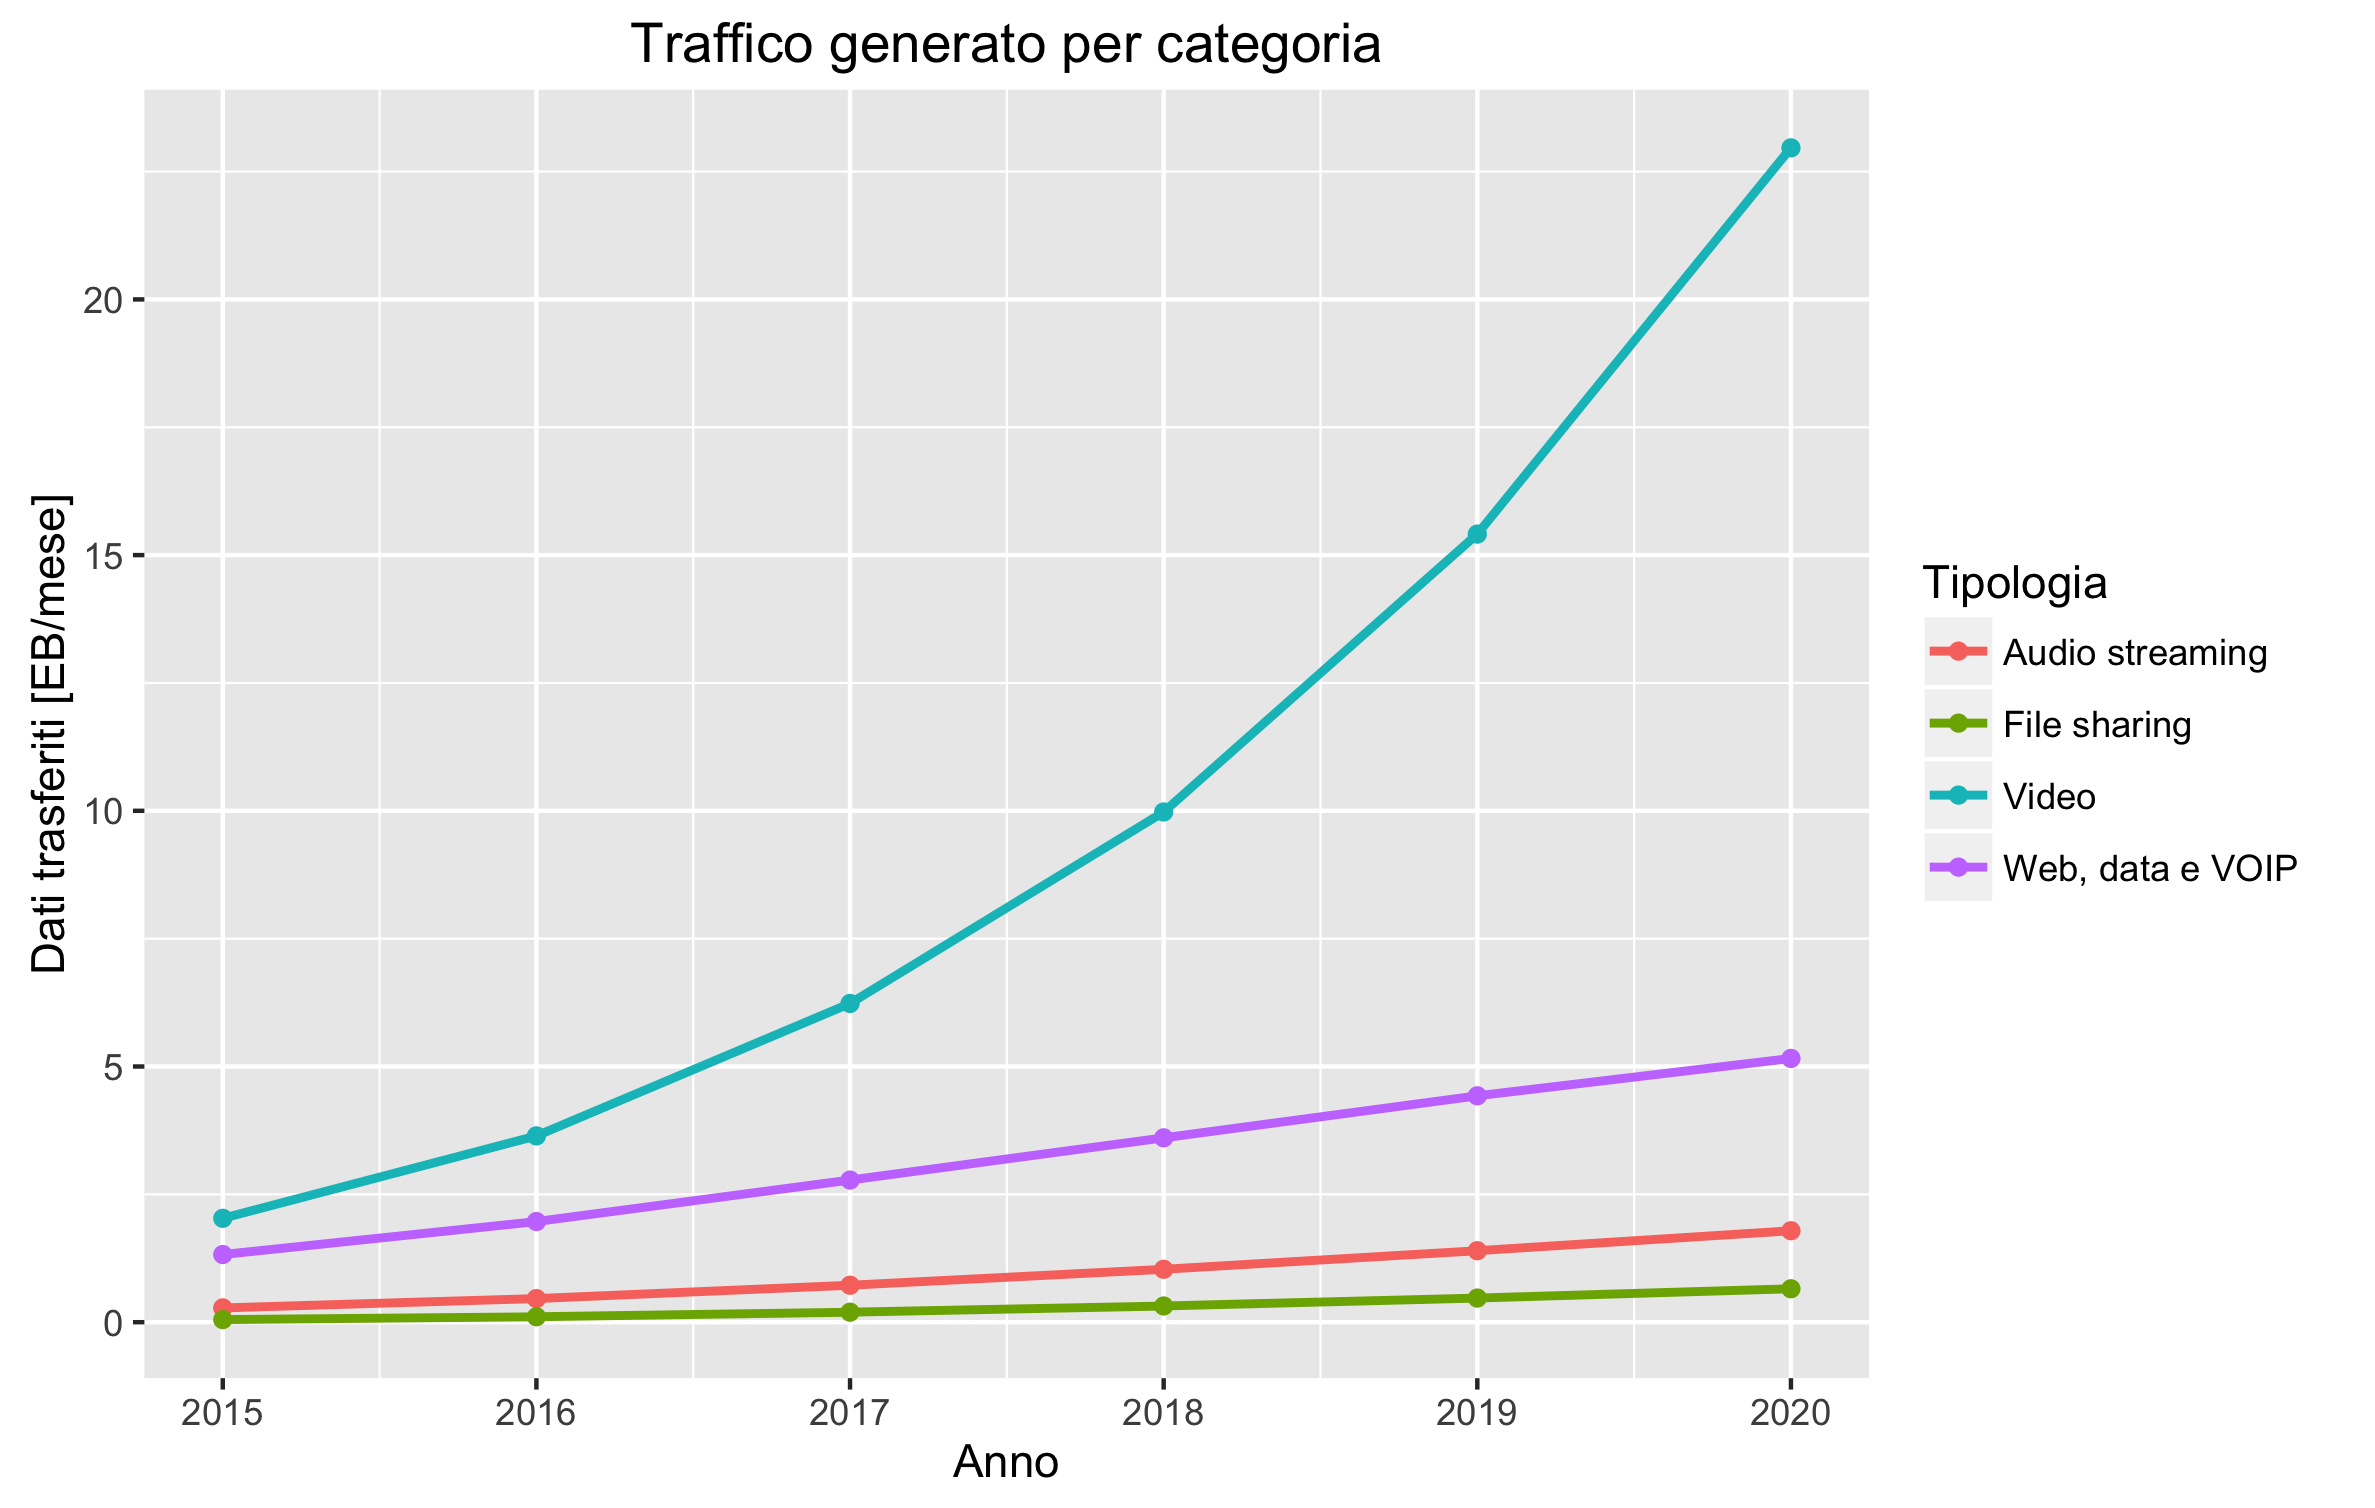
\includegraphics[width=\textwidth]{1-introduzione/Immagini/traffico-categoria.png}
	\caption[Traffico generato per categoria di applicazione]{Traffico generato per categoria di applicazione (fonte: Cisco, 2016)\label{fig:traffico-categoria-applicazione}}
\end{figure}

Internet è diventato una fonte immensa di informazioni, che sono destinate ad aumentare. Un recente trend è relativo ai dispositivi connessi, definito \emph{Internet of Things} (Figura \ref{fig:statistiche-iot}). L'idea è che qualsiasi dispositivo può essere connesso a Internet per generare informazioni, in particolare tutti quelli provvisti di \emph{sensori} che possono fornire dati sullo stato dell'ambiente nel quale si trovano.

\begin{figure}[ht]
	\centering
	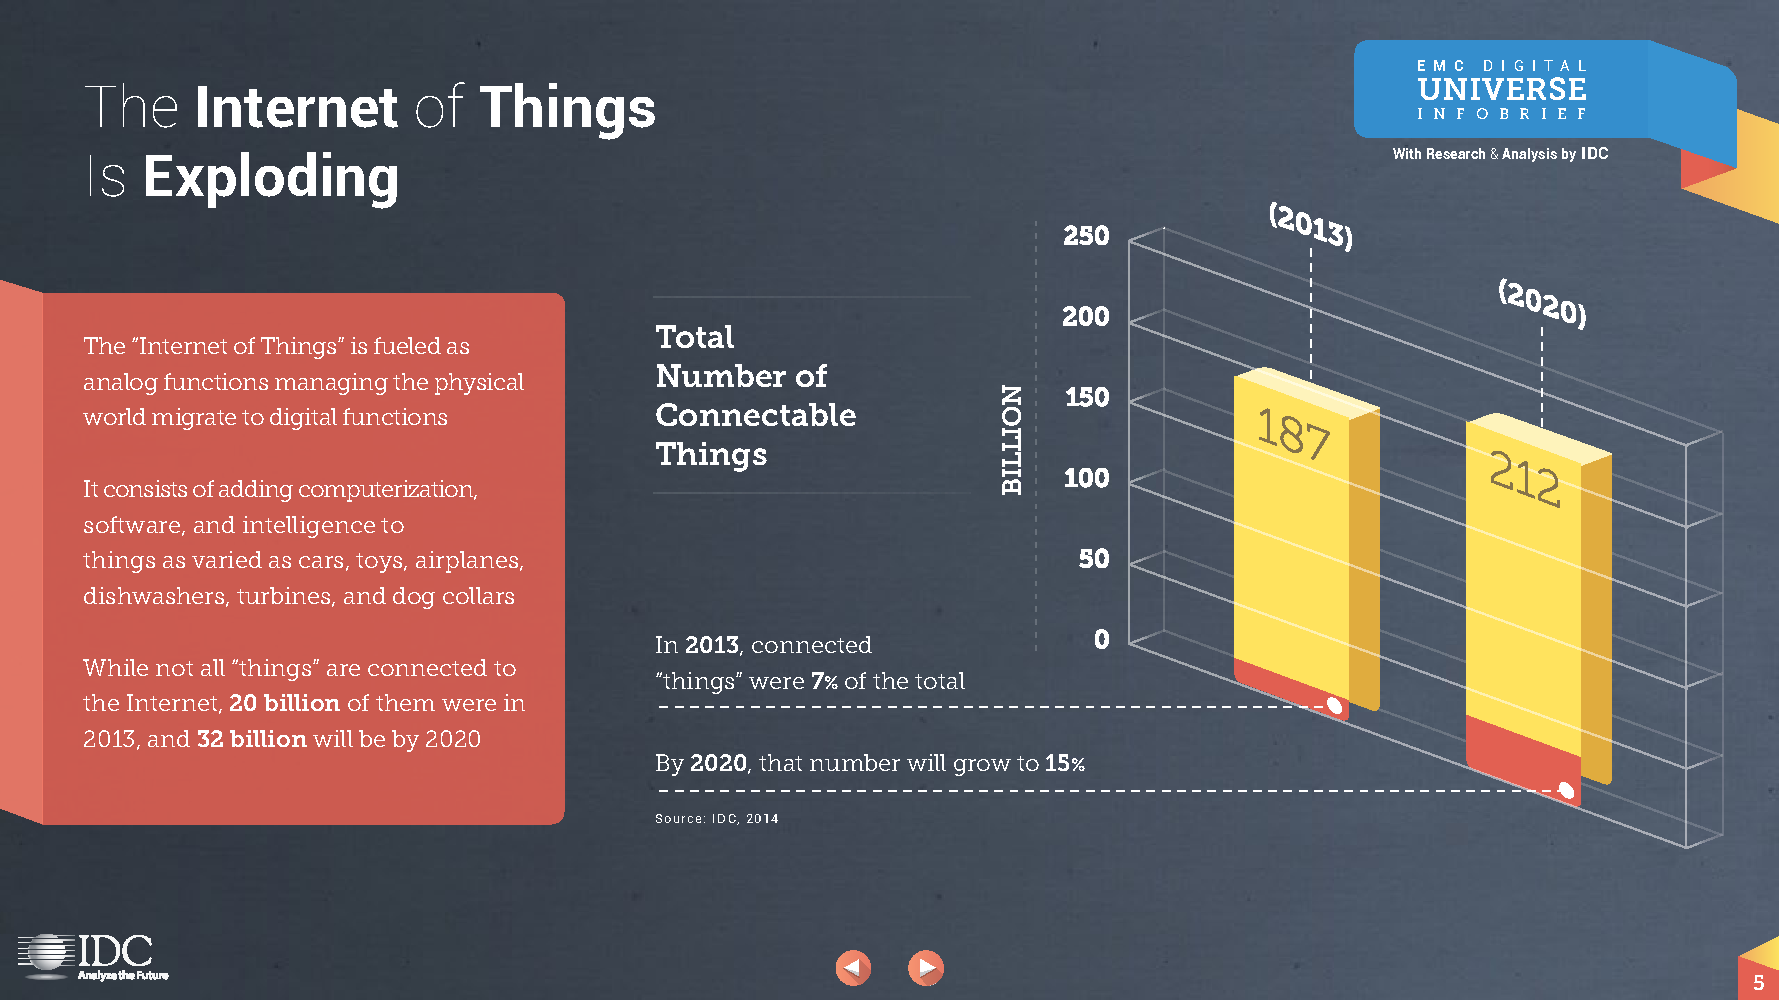
\includegraphics[width=\textwidth]{1-introduzione/Immagini/iot-trend.pdf}
	\caption[Statistiche sull'Internet of Things]{Statistiche sull'Internet of Things (fonte: IDC, 2014)\label{fig:statistiche-iot}}
\end{figure}

%Inizio parte del contesto
Uno dei principali problemi che chiunque lavori coi dati vuole cercare di risolvere è ridurre l'\emph{information noise}, migliorando la precisione delle informazioni da mostrare, in maniera che meglio si adattino ai requisiti.

\upe frequente che le informazioni non vengano acquisite unicamente da una base di dati bensì provengano da più fonti, anche di tipologie diverse tra loro (es.: relazionali, XML, ec..). Basti pensare alla moltitudine di servizi presenti nel web.

Questo aumento della quantità di informazioni, se non propriamente controllato, può provocare un ammasso di dati che genera soltanto confusione piuttosto che fornire elementi utili, riducendo i benefici che invece si potrebbero ricavare da tutte queste informazioni. Tuttavia, distinguere le informazioni rilevanti da quelle che non lo sono è un compito tutt'altro che semplice: alcune informazioni potrebbero essere trattate in maniera differente, anche per lo stesso utente, che in diverse situazioni ha bisogno di informazioni differenti. 

Si parla dunque di sistemi \emph{context aware}, che si occupano dell'\emph{acquisizione} del contesto (per esempio tramite l'utilizzo di determinati sensori), l'\emph{astrazione} e il \emph{riconoscimento} del contesto (per esempio associare un determinato stimolo al contesto) e il \emph{comportamento} adatto alla situazione riconosciuta (per esempio l'esecuzione di un'azione innescata dal contesto) \cite{schmidt2003ubiquitous}. L'utilizzo del \emph{contesto} permette la realizzazione di interfacce grafiche innovative e viene spesso utilizzato nella \emph{computazione ubiqua} e nei \emph{dispositivi indossabili}.

%Resta aperto il problema di come visualizzare le operazioni e come ricercare le info in modo semplice (Fornire interfaccia per permettere agli utenti di cercare le informazioni)

Una volta acquisite le informazioni nasce l'esigenza di definire regole su come mostrarle all'utente finale. Con la diffusione di dispositivi mobili sempre più sofisticati si è resa maggiormente necessaria un'esperienza utente semplice che lo guidi durante le sue attività .

%	parlare di come sia conveniente un meccanismo decori le informazioni testuali con contenuti aggiuntivi, come mappe, foto e altre cose dinamiche}

Per questo motivo ha assunto un ruolo di grande importanza l'esperienza d'uso dell'utente (\emph{User Experience}). Infatti se un'applicazione non è ben formata e non è fruibile in modo semplice dall'utente, il numero di utenti che la utilizzeranno calerà sempre di più. Secondo Gary Illyes di Google \virgolette{circa il 61 percento degli utenti che incontrano problemi con siti e app su smartphone ne abbandonano l'utilizzo volontariamente}\footnote{Search Engine Land Interview to Gary Illyes of Google: \url{http://searchengineland.com/google-may-add-mobile-user-experience-ranking-algorithm-205382}}. Per evitare questo problema è necessario prestare un'attenzione sempre maggiore a come viene progettato tutto il flusso di navigazione dell'utente e a fornirgli i dati necessari per poter sfruttare al meglio l'applicazione. L'aggiunta di elementi comprensibili in modo intuitivo come mappe e foto porta l'utente a utilizzare altre aree della mente, come quella della memoria fotografica. In questo modo l'utente può facilmente acquisire conoscenza utilizzando diversi dati e diverse tipologie di visualizzazione.

%inizio parte di progetto

\upe proprio per cercare nuovi strumenti in grado di migliorare l'esperienza dell'u\-ten\-te nell'esplorazione delle informazioni che nasce il progetto CAMUS. CAMUS (\emph{Context Aware Mobile mashUpS}) si propone come un \emph{framework} per permettere la realizzazione di app mobili che si adattino sia alle preferenze dell'utente sia alla situazione nella quale si trova. L'idea è che l'utilizzo di modelli per definire il contesto e per schematizzare la composizione dell'interfaccia grafica possa portare enormi benefici nell'interazione tra utente e applicazione.

Questo paradigma permette la realizzazione di applicazioni flessibili e personalizzate dove la struttura e i contenuti possono variare in fase di esecuzione in base alle esigenze dell'utente e alla situazione nella quale si trova. Inoltre si vuole sfruttare la multimedialità messa a disposizione dei recenti dispositivi mobili per coinvolgere maggiormente l'utente e semplificargli le attività.

Dalla sigla è possibile intuire le due anime principali che sono alla base del progetto: i \emph{mashup} e il \emph{contesto}.

Per la tematica dei \emph{mashup} viene preso in considerazione l'aspetto di acquisire le informazioni da più fonti di diverso tipo. CAMUS prevede un sistema flessibile che permette di acquisire informazioni da diverse fonti, andando così ad aumentare il potere conoscitivo che si può fornire all'utente. Come detto in precedenza bisogna stare particolarmente attenti all'utilizzo di grosse quantità di dati, in quanto se non opportunamente trattate e filtrate possono generare solamente confusione e risultare così poco fruibili dall'utente. Nasce così l'intuizione di utilizzare il contesto come metodo di selezione dei dati che sono più rilevanti per l'utente. Il contesto mette a disposizione lo stato in cui si trova l'utente, le condizioni dell'ambiente che lo circonda e i suoi interessi personali. Si ritiene che queste preziose informazioni possano essere uno strumento determinante per mettere ordine ai dati e fornire così solo le informazioni che sono interessanti.

Nella tesi si andrà ad affrontare la modellazione della situazione nella quale si trova l'utente. \upe un'attività molto delicata, in quanto esistono una moltitudine di parametri che possono definire una particolare situazione. \upe necessario fare una scelta di quali siano gli indicatori più idonei e quali invece possano essere scartati. L'obiettivo è fornire un modello che permetta di definire in maniera adeguata e \emph{semplice} il contesto in modo da agevolare l'utente nell'attività, rispettando i principi di \emph{User Experience} precedentemente citati.

Certamente il problema principale riguarda l'organizzazione fisica delle informazioni. Visto che CAMUS non viene limitato ad uno specifico contesto, è necessario prevedere un meccanismo che permetta di adattare la visualizzazione di categorie diverse di informazioni. Come è facilmente intuibile mostrare un elenco di film è ben diverso da mostrare un elenco di ristoranti. Un primo punto da snodare è quindi relativo alla creazione di uno schema flessibile che permetta di descrivere come visualizzare queste informazioni sul dispositivo.

Ma non solo: questo schema deve essere anche in grado di raccogliere informazioni di contorno che permettano di migliorare l'esplorazione di quelle principali. Per esempio, se si sta cercando un ristorante può essere d'aiuto avere a disposizione una galleria di foto del locale con i piatti che offre, una mappa che indichi dove si trova il ristorante o alcune informazioni sul meteo, per decidere se prenotare all'esterno o all'interno. Invece se si sta cercando un film può essere sicuramente d'aiuto avere un trailer da vedere per farsi un'idea del film oppure l'elenco dei cinema che l'hanno in programmazione.

Quelle descritte sono operazioni non sempre alla portata degli utenti, soprattutto per quanto riguarda la modellazione del contesto o la composizione dell'interfaccia grafica. Inoltre, quando il contesto diventa in grado di descrivere diverse realtà, assume anche dimensioni notevoli. Avere troppe scelte a disposizione rende vani gli sforzi per cercare di mettere ordine nei dati, in quanto verrebbe solamente spostato il problema a un altro livello. L'utente non conosce a fondo la struttura dei dati e non è in grado quindi di comporre al meglio un'interfaccia completa dei servizi ausiliari. Per agevolare l'utente in queste situazioni si è deciso di dare importanza alla figura dell'\emph{esperto di settore}. L'esperto di settore è colui che conosce a fondo l'ambito di utilizzo di una \emph{CAMUS app}. Si ritiene che questa sua conoscenza permetta di guidare l'utente nelle sue scelte. Uno dei suoi compiti sarà quello di definire insieme all'utente un profilo, in base alle sue esigenze, in modo che dal contesto possano essere eliminati i rami non necessari. Inoltre si occuperà di comporre delle interfacce funzionali sia per la situazione sia per l'utente. In questo modo è possibile avere una varietà di composizioni adatte ai diversi ambiti di utilizzo che si adattino anche alle preferenze dell'utente e ad altri fattori, come la località.

All'esperto di settore vengono delegati compiti che riguardano maggiormente l'ambito nel quale viene utilizzata l'applicazione. Per questo motivo non è necessario che sia una figura con particolari competenze informatiche. Nel \emph{framework} però saranno necessarie delle fasi più tecniche, per il corretto funzionamento della piattaforma. Queste attività sono relative alle configurazioni del sistema, che necessitano di competenze soprattutto per quanto riguarda il funzionamento dei servizi. Per questo motivo si è scelto di introdurre la figura dell'\emph{amministratore}. I suoi compiti sono quelli di creare lo schema globale del contesto, che verrà utilizzato dagli esperti di settore per creare gli schemi personalizzati, e la descrizione dei servizi che il sistema può usufruire per recuperare le informazioni. Può anche dedicarsi all'introduzione di nuovi componenti utilizzabili nella fase di composizione degli schemi visuali.

\section{Caso di studio: il turismo\label{sec:caso-studio-turismo}}

In questa sezione viene introdotto un caso di studio, che serve per validare il modello proposto per CAMUS. Utilizzare un esempio di applicazione del framework a un caso reale può essere un utile indicatore al fine di supportare le scelte effettuate e di osservare se sono presenti alcune lacune nella modellazione.

CAMUS ha come obiettivo quello di essere universale, cioè utilizzabile in ambiti anche molto diversi tra loro. Come caso di studio è stato dunque necessario pensare a un ambito che consentisse di sfruttare al meglio le capacità di adattarsi alle varie situazioni nelle quali si può trovare l'utilizzatore dell'app.

\upe stato scelto il caso di studio relativo al settore \emph{turistico}, proprio per via della sua dinamicità. In particolare si è preso in considerazione il caso di un'agenzia di viaggi che deve proporre ai propri clienti dei pacchetti di viaggio.

L'ambito turistico calza a pennello per gli intenti di CAMUS; un viaggio incomincia dalla sua pianificazione: prima di partire, il turista si informa sulla destinazione, quali hotel sono disponibili, con quali mezzi di trasporto è più conveniente raggiungere la destinazione, ecc. In questo frangente CAMUS si propone come \virgolette{suggeritore} di esperienze di viaggio: permette all'utente di non concentrarsi sul \emph{dove} vuole andare, ma sul \emph{cosa} vuole fare. Gli viene data la possibilità di scegliere l'esperienza di viaggio che vuole intraprendere e proporgli così i pacchetti che corrispondono alle sue scelte.

Le potenzialità di CAMUS non terminano una volta che il viaggiatore sceglie la sua meta: l'app gli servirà \emph{durante} il viaggio per informarsi sulle attività da svolgere, le escursioni disponibili, i ristoranti nei quali cenare, ecc. Per esempio, se un utente vuole provare un ristorante tipico della zona, gli basterà aprire l'app CAMUS e selezionare che è interessato nella ricerca dei ristoranti che propongono dei menù \emph{tipici} del luogo. Gli verrà mostrato un elenco dei ristoranti che si trovano nei suoi paraggi che rispettano i criteri definiti. Inoltre gli verranno fornite indicazioni su come raggiungere il ristorante, sfruttando, se specificato nella richiesta, i mezzi pubblici presenti nella destinazione scelta.

Le due figure principali in questo caso di studio sono due: l'\emph{agente di viaggio} e il \emph{turista}. L'\emph{agente} ha il compito di organizzare tutto il viaggio, gestire quindi le prenotazioni, gli spostamenti principali e i soggiorni per il viaggiatore, mentre il \emph{turista} è colui che fisicamente compie il viaggio, che può essere quindi considerato come l'utente finale.

All'agente vengono inoltre demandati i compiti di personalizzazione dell'app: questa fase avviene quando il cliente si presenta nell'agenzia di viaggio. A quest'ultimo vengono prima di tutto fatte alcune domande per conoscere il suo profilo, in modo da adattare le scelte che gli verranno mostrate dall'app. In questo modo è possibile evitare che al cliente vengano proposte troppe scelte che non siano di suo interesse. Inoltre vengono fissate alcune opzioni che tendono a non cambiare nel corso del viaggio; per esempio se l'utente viaggia con un animale domestico questa scelta sarà sempre la stessa durante tutto il viaggio e non gli verrà chiesta di nuovo.%\footnote{CAMUS si schiera contro l'abbandono degli animali: \url{http://www.emergenza24.org/salvaunamico/}}

L'ulteriore compito che può svolgere l'agente è quello di personalizzare l'aspetto grafico dell'app qualora ritenga che sia necessario. Con CAMUS vengono proposti alcuni template predefiniti per ogni categoria e viene lasciata libera scelta all'agente se utilizzarli così come sono o modificarli. Una delle motivazioni nella scelta di modificare l'aspetto riguarda l'aggiunta di alcuni servizi di supporto. Per esempio, se l'agente è consapevole che nel luogo in cui vuole andare il cliente le condizioni meteorologiche sono molto variabili e nella versione predefinita dell'app non sono presenti informazioni meteo, può aggiungere questa indicazione in modo da fornire al turista un'informazione in più per gestire al meglio la sua vacanza.

Come si può notare da questo breve esempio, l'utilizzo di CAMUS in un'agenzia viaggi permette di fornire un servizio più coinvolgente ai propri clienti. La realizzazione di app personalizzate appositamente per un turista permette di effettuare scelte migliori e di proprio interesse. Inoltre estende la capacità dell'agenzia di fornire un'assistenza al proprio cliente anche durante il viaggio: si può affermare che un'app CAMUS assume il ruolo di \emph{assistente di viaggio} e guida il turista durante tutte le fasi della sua esperienza di viaggio.

\section{Struttura della tesi}

Viene ora fornita una panoramica sulla struttura di questa tesi:

\begin{itemize}
	\item 
	Nel Capitolo \ref{ch:nozioni-preliminari}, dopo aver introdotto i modelli e le tecnologie che saranno utilizzate nel resto della tesi, si discute la letteratura sull'argomento e le tecnologie impiegate per lo sviluppo del prototipo
	\item 
	Nel Capitolo \ref{ch:metodologia-camus} si entra nei dettagli del progetto CAMUS andando a fornire un contesto più ampio di quello appena descritto e mettendo in risalto gli obiettivi che si vogliono raggiungere. In seguito saranno analizzate nel dettaglio le logiche alla base del \emph{framework}
	\item 
	Nel Capitolo \ref{ch:progettazione-alto-livello} viene introdotta l'architettura della piattaforma. Verrà inoltre fornito uno schema del flusso di esecuzione delle attività ed esposto un caso d'uso reale per chiarire meglio la sequenza delle attività
	\item 
	Nei Capitoli \ref{ch:implementazione-backend} e \ref{ch:implementazione-app} viene analizzata nel dettaglio l'implementazione rispettivamente lato \emph{backend} e \emph{mobile app}. Si analizzano i componenti che formano il sistema e le scelte tecnologiche che hanno portato alla realizzazione del prototipo
	\item 
	Nel Capitolo \ref{ch:performance} si andranno ad analizzare le prestazioni della soluzione implementata, simulando alcuni casi d'uso simili alle condizioni di regime della piattaforma
	\item 
	Nel Capitolo \ref{ch:conclusioni} si discuteranno le conclusioni del lavoro relativo al progetto e alcuni spunti per futuri miglioramenti al framework
\end{itemize}


\chapter{Nozioni preliminari\label{ch:nozioni-preliminari}}


In questo capitolo vengono esposti i concetti alla base del progetto CAMUS. In questo modo viene fornito al lettore un quadro generale delle tematiche che verranno affrontate nei successivi capitoli. Il capitolo inizia con l'introduzione del concetto di \emph{context awareness}, che � la prima delle due anime del progetto, seguita dalla presentazione del modello del contesto che viene utilizzato in CAMUS, il \emph{Context Dimension Tree}. Successivamente viene presentato il secondo pilastro del progetto, i \emph{mashup}, ed in particolar modo la tipologia di nostro interesse, i \emph{mobile mashup}. Di seguito verranno analizzate le varie tipologie di \emph{servizi} che il web mette a disposizione. La loro posizione non deve trarre in inganno: i servizi sono egualmente importanti in quanto permettono all'intero sistema di funzionare: infatti forniscono le informazioni che vengono presentate all'utente; senza servizi l'intero progetto non sarebbe altro che un'impalcatura fine a se stessa. Infine viene effettuato un confronto con i principali competitor di CAMUS, cio� tutti i lavori esistenti che affrontano le medesime tematiche.

\section{Context-Awareness\label{sec:context-awareness}}

Il concetto di \emph{contesto} viene citato in diverse aree di ricerca, come la filosofia, la psicologia e l'informatica. Il \emph{contesto} gioca spesso un ruolo importante nel definire un comportamento o l'interpretazione dell'ambiente; dei cambiamenti nel contesto possono cambiare la percezione del momento che si sta vivendo. La parola \virgolette{contesto} deriva dalle parole latine \emph{con} e \emph{texere}, che significa tessere intrecciate, intrecciare. Viene definito come \virgolette{il complesso delle circostanze e delle situazioni nelle quali un fatto o un fenomeno si verificano}\footnote{Dizionario Garzanti: \url{http://www.garzantilinguistica.it/ricerca/?q=contesto}}.

In informatica il concetto di \emph{contesto} � riferito all'idea che i computer possano avere una percezione dell'ambiente e che riescano dunque a modificare il loro comportamento in base alla situazione. I dispositivi devono dunque acquisire informazioni relative l'ambiente in cui operano e tramite determinate regole, che possono essere sia staticamente fissate che dinamicamente dedotte tramite algoritmi di intelligenza artificiale, riescano a reagire di conseguenza, utilizzando la strategia pi� idonea alla situazione corrente. Il termine \emph{context awareness} � stato introdotto per la prima volta in ambito informatico ad opera di Schilit \cite{schilit1994context}\cite{schilit1994disseminating}.

Agli albori il \emph{contesto} veniva inteso solamente come la posizione nella quale si trova l'utente, come discusso da Dey in \cite{dey2001understanding}; negli ultimi anni invece si � iniziato a pensare al \emph{contesto} non solo come uno stato, bens� come un processo pi� vasto che coinvolge diversi aspetti relativi all'utente. Sono stati dunque ideati modelli di \emph{contesto} sofisticati e generali, in modo che possano adattarsi a diverse situazioni d'utilizzo \cite{DBLP:journals/sigmod/BolchiniCQST07} \cite{baldauf2007survey}.

In particolare il \emph{contesto} viene utilizzato per realizzare applicazioni che siano in grado di \emph{a)} adattare l'interfaccia grafica, \emph{b)} filtrare l'insieme dei dati che sono realmente rilevanti, \emph{c)} migliorare la precisione dei dati raccolti, \emph{d)} scoprire servizi, \emph{e)} predirre alcune scelte dell'utente o \emph{f)} realizzare ambienti \emph{intelligenti}.

Si prenda come esempio un dispositivo mobile fornito ai visitatori di un museo di storia naturale che sfrutti il contesto per \emph{a)} adattare la struttura e l'aspetto dell'interfaccia grafica in base alle caratteristiche del visitatore, sia esso una persona con problemi di vista oppure un bambino; \emph{b)} mostrare informazioni diverse in base agli interessi del visitatore (es.: geologia, paleontologia, ecc.) oppure in base alla stanza in cui si trova; \emph{c)} imparare dalle precedenti scelte effettuate dall'utente su quali potranno essere le informazioni di maggiore gradimento; \emph{d)} proporre al visitatore determinati servizi, come l'acquisto dei biglietti per una mostra temporanea o la prenotazione di un posto nello spettacolo sui dinosauri che sta per incominciare nella sala adiacente; \emph{e)} conoscere la posizione del visitatore in base ai sensori che monitorano l'ambiente; \emph{f)} fornire dei contenuti attivi al visitatore sul cosa accade in un particolare ambiente.

I sistemi \emph{context aware} riguardano l'\emph{acquisizione} del contesto (per esempio tramite l'utilizzo di determinati sensori), l'\emph{astrazione} e il \emph{riconoscimento} del contesto (per esempio associare un determinato stimolo al contesto) ed il \emph{comportamento} adatto alla situazione riconosciuta (per esempio l'esecuzione di un'azione innescata dal contesto) \cite{schmidt2003ubiquitous}. L'utilizzo del \emph{contesto} permette la realizzazione di interfacce grafiche innovative e viene spesso utilizzato nella \emph{computazione ubiqua} e nei \emph{dispositivi indossabili}.

Nella seguente sezione verr� presentato nel dettaglio il \emph{Context Dimension Model}, un modello di contesto che sfrutta una struttura ad albero per descrivere la situazione nel quale si trova l'utente. Tra la moltitudine di alternative esistenti viene presentato questo modello in particolare perch� � quello che verr� utilizzato nel progetto CAMUS, quindi la comprensione della sua rappresentazione e delle potenzialit� saranno utili per i successivi capitoli.

\subsection{Context Dimension Model\label{sec:context-dimension-model}}

In questa sezione viene presentato nel dettaglio il \emph{Context Dimension Tree} \cite{DBLP:journals/is/BolchiniQT13}, in quanto � il modello di rappresentazione del contesto che � stato selezionato per l'utilizzo nel progetto CAMUS. Nel \emph{Context Dimension Model} il contesto viene rappresentato come un albero $\mathcal{T} = \textless N, E, r \textgreater $, che descrive i possibili contesti nei quali ci si pu� trovare in una data situazione. \`E formato da una radice \emph{r} e un insieme di nodi \emph{N}, che vengono partizionati nei sottoinsiemi dei \emph{nodi dimensione} $N_D$, colorati di nero, e nei \emph{nodi concetto} $N_C$, colorati di bianco, che rappresentano i possibili valori che possono assumere le dimensioni e dall'insieme dei collegamenti tra i nodi \emph{E}. La radice \emph{r} � un \emph{nodo concetto}, in quanto rappresenta il contesto pi� generale possibile, che corrisponde dunque all'intero dataset.

\begin{figure}[h]
	\centering
	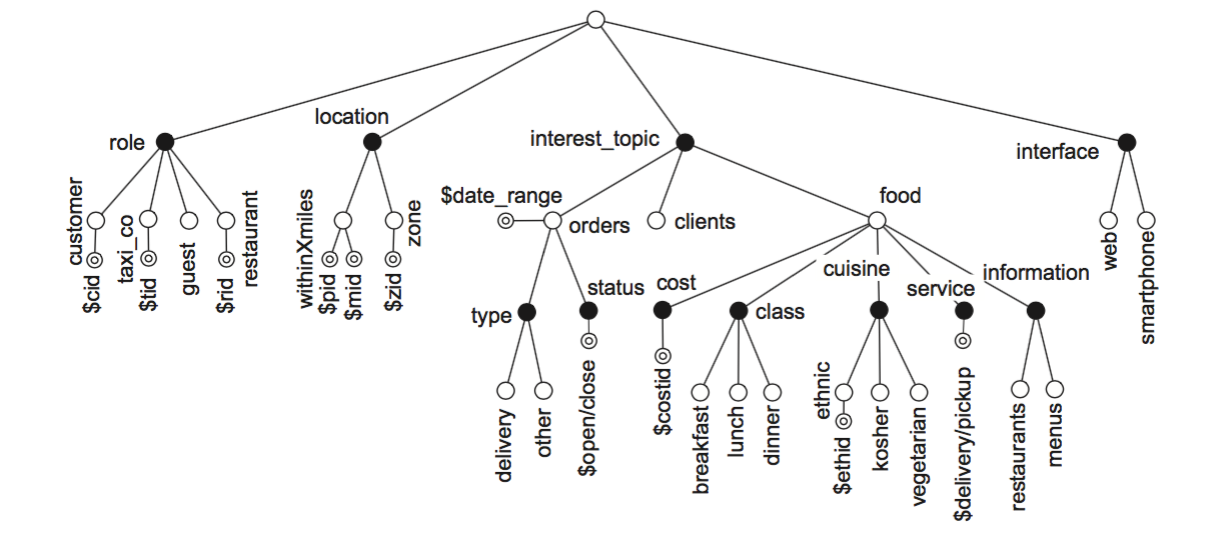
\includegraphics[width=\textwidth]{2-nozioni-preliminari/Immagini/esempio_cdt.png}
	\caption{Context Dimension Tree}\label{fig:context-dimension-tree}
\end{figure}

Le dimensioni che sono dirette discendenti della radice vengono chiamate \emph{dimensioni principali}, perch� definiscono le differenti caratteristiche dell'utente e del contesto nel quale agiscono. Nell'esempio in Figura \ref{fig:context-dimension-tree}, le \emph{dimensioni principali} sono il \emph{ruolo} dell'utente, l'\emph{interfaccia} tramite la quale accede ai dati, l'\emph{interest topic} e la \emph{posizione} in cui si trova. Inoltre, ogni valore pu� essere ulteriormente specializzato tramite \emph{sottodimensioni}, che a loro volta formano un sottoalbero. Per esempio, l'interest topic \virgolette{ordine} pu� essere analizzato in base allo \emph{stato} in cui si trova oppure in base alla sua \emph{tipologia}.

Ogni nodo del CDT � caratterizzato dalla sua tipologia, che pu� essere \emph{dimensione} o \emph{concetto}, e dalla sua etichetta; pu� essere identificato univocamente tramite l'unico percorso che lo collega fino alla radice. Senza perdita di generalit�, viene adottata l'ipotesi che ogni etichetta sia unica in un albero, quindi ogni nodo pu� essere identificato semplicemente dalla sua etichetta. I collegamenti tra i vari nodi non vengono invece etichettati.

L'alternanza tra nodi \emph{dimensione} e \emph{concetto} fa s� che vengano create delle \emph{generazioni}, ognuna delle quali sar� formata da nodi dello stesso colore, e ogni colore verr� alternato man mano che si prosegue discendendo nell'albero: dunque ogni \emph{nodo dimensione} pu� avere come figli solo nodi di tipo \emph{concetto} e viceversa.

\`E inoltre possibile associare uno o pi� \emph{parametri} ai nodi concetto e ai nodi dimensione che sono foglie dell'albero. Ogni parametro permette di raffinare ulteriormente la selezione dei dati e selezionare un sottoinsieme del dataset particolare. Per esempio, il parametro \virgolette{intervallo} associato al concetto \emph{ordini} permette di indicare un intervallo di date e quindi di selezionare esclusivamente gli ordini che sono riferiti alle date indicate.

Per ogni \emph{nodo dimensione} � possibile selezionare al massimo un nodo concetto tra i suoi figli oppure, se non possiede alcun nodo figlio, deve essere selezionato obbligatoriamente uno ed un solo parametro. L'utilizzo dei \emph{parametri} aumenta il potere espressivo del modello, in quanto lo rende pi� semplice per l'utilizzo da parte del designer. Si � resa necessaria l'introduzione dei parametri in quanto non tutti i concetti espressi da una dimensione possono essere enumerati. Per esempio, la dimensione \virgolette{costo} pu� assumere infiniti valori ed � quindi pi� appropriato l'utilizzo di un parametro che sia variabile.

Ora che � stato definito il modello � necessario spiegare come viene rappresentato uno specifico \emph{contesto}. Dato un \emph{Context Dimension Tree} $\mathcal{T} = \textless N, E, r \textgreater $, un \emph{contesto} � definito dalla seguente grammatica con assioma \emph{context}:

\begin{equation*}
	C =
	\begin{cases}
		\textless context \textgreater \leftarrow \textless context\_element \textgreater\ |\ \textless context\_element \textgreater \land \textless context \textgreater\\
		\textless context\_element \textgreater \leftarrow dim\_name: \textless value\_item \textgreater\ |\ dim\_name\ (\textless parameter \textgreater)\\
		\textless value\_item \textgreater \leftarrow value\ |\ value\ (\textless parameters \textgreater)\\
		\textless parameters \textgreater \leftarrow \textless parameters \textgreater \land \textless parameter \textgreater\ |\ \textless parameter \textgreater\\
		\textless parameter \textgreater \leftarrow param\_name: param\_value
	\end{cases}
\end{equation*}

Un \emph{contesto} � formato dalla congiunzione tra uno o pi� \emph{elementi del contesto}. Ogni elemento del contesto � formato dal nome della dimensione seguita da uno dei valori scelto tra i nodi che sono suoi figli diretti, oppure dal valore che assume l'unico parametro ad essa associato, nel caso in cui la dimensione � una foglia dell'albero. Ogni valore pu� essere a sua volta raffinato aggiungendo il/i parametro/i ad esso associati.

Non � necessario selezionare per forza tutte le dimensioni presenti nell'albero: non selezionare alcun valore relativo ad una dimensione equivale ad essere indifferenti rispetto quella particolare situazione. Ogni dimensione che non viene selezionata non influir� nel processo di acquisizione dei dati contestuali.

Un esempio di contesto �:

\begin{align*}
	C =\ &role : customer\ (\$cid : ``Bill")\ \land \\
		&interest\_topic : orders\ \land \\
		&interface : smartphone
\end{align*}

che rappresenta il contesto in cui il cliente Bill � interessato nel ricevere informazioni sui propri ordini sullo smartphone. Il contesto \emph{C} � quindi composto da tre elementi del contesto.

Infine, dopo aver discusso del modello e di come vengono rappresentati i vari contesti, resta da definire come � possibile acquisire i dati che sono pertinenti ad un determinato contesto. Come evidenziato in \cite{DBLP:journals/cacm/BolchiniCOQRST09}, esistono due strategie principali per definire le associazioni tra i contesti e la porzione di dati rilevanti per i vari contesti, chiamate \emph{configuration-based mapping} e \emph{value-based mapping}.

\begin{figure}[h]
	\centering
	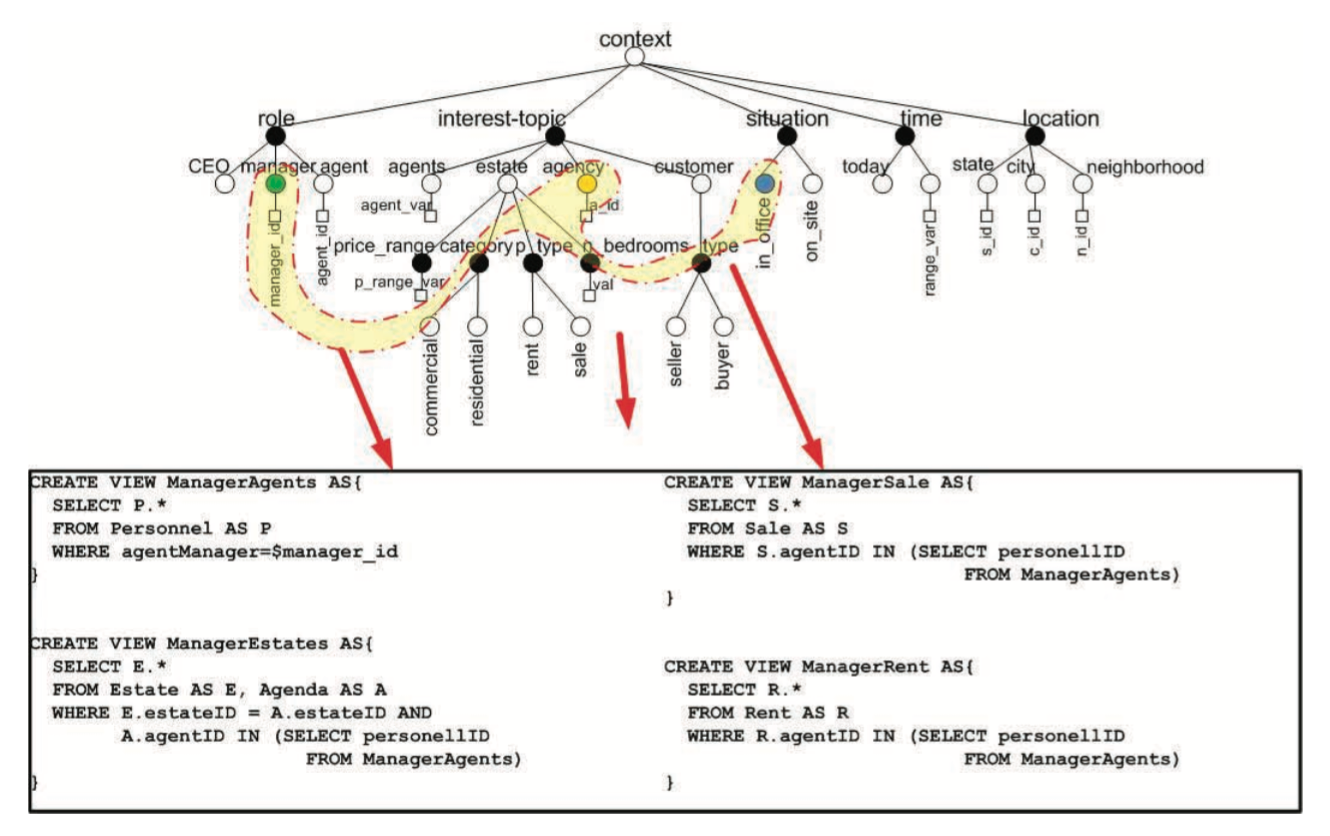
\includegraphics[width=\textwidth]{2-nozioni-preliminari/Immagini/configuration-based-mapping.png}
	\caption{Configuration-based mapping}\label{fig:configuration-based-mapping}
\end{figure}

La strategia \emph{configuration-based mapping} prevede che il designer definisca per ogni contesto possibile la relativa porzione del dataset da mostrare. Questa operazione pu� essere effettuata definendo delle viste nel linguaggio specifico del database adottato. In Figura \ref{fig:configuration-based-mapping} viene mostrato un esempio per il contesto nel quale un manager � interessato alle informazioni relative le sue agenzie. In questo caso il designer specifica delle viste in linguaggio SQL relative al contesto specifico, mettendo in evidenza i dati del personale che lavora nelle agenzie gestite dal manager, i contratti di affitto e vendita ed infine le informazioni relative alle propriet�.

Questa strategia ha il vantaggio di generare delle viste molto precise rispetto al contesto che vogliono rappresentare, ma ha l'enorme svantaggio che deve essere ripetuta per ognuno dei possibili contesti che, com'� facilmente intuibile, possono essere in quantit� molto elevata. Inoltre, se in futuro dovesse essere aggiunta un'ulteriore dimensione, sarebbe necessario modificare le varie associazioni per includere la nuova dimensione.

\begin{figure}[h]
	\centering
	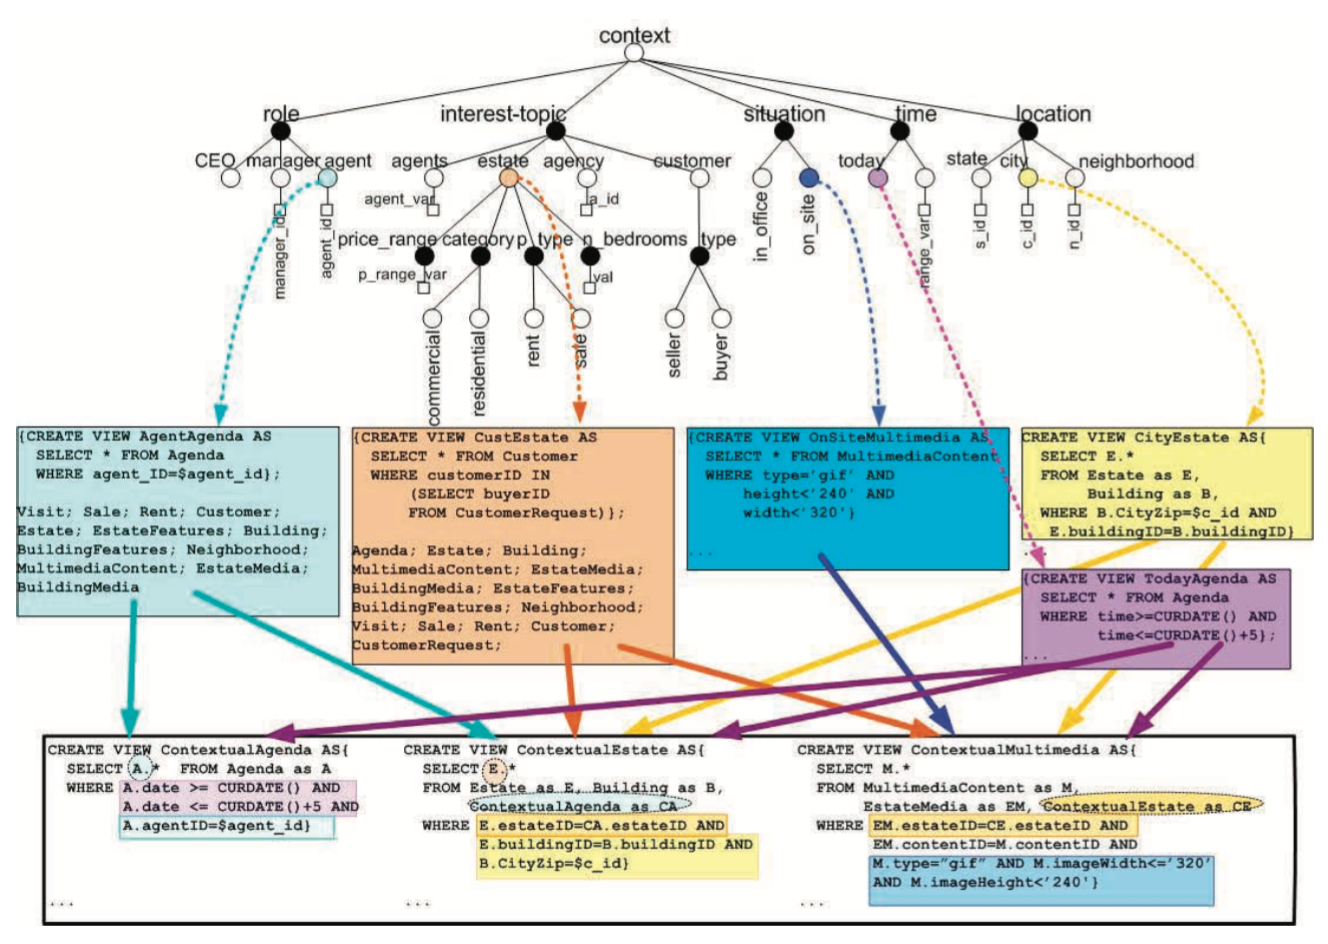
\includegraphics[width=\textwidth]{2-nozioni-preliminari/Immagini/value-based-mapping.png}
	\caption{Value-based mapping}\label{fig:value-based-mapping}
\end{figure}

La strategia \emph{value-based mapping} permette di superare i limiti evidenziati per la strategia precedente. Questa strategia prevede che il designer definisca le viste parziali relative ad un particolare elemento del contesto, indipendentemente dagli altri. Quindi, una volta selezionato un contesto, un algoritmo si occuper� di combinare assieme le varie viste parziali definite dai singoli elementi per formare la vista globale adatta allo specifico contesto. La Figura \ref{fig:value-based-mapping} mostra come il contesto dell'esempio precedente viene mappato tramite questa strategia. Le linee tratteggiate mostrano le viste parziali che vengono associate ai vari elementi del contesto, mentre nel riquadro in basso viene mostrata la vista globale generata dalla combinazione delle viste parziali. L'algoritmo di composizione delle view parziali � basato sull'utilizzo di diverse policy e operatori di composizione, tra i quali i pi� utilizzati sono \emph{double union}, \emph{double intersection} e \emph{double difference} \cite{DBLP:conf/er/BolchiniQR07}.

\section{Mashup\label{sec:mashup}}

In questa sezione vengono introdotti i \emph{Mashup}, la seconda anima del sistema CAMUS, e il loro ruolo nell'applicazione finale.
La parola \emph{Mashup}, che significa letteralmente miscuglio o combinazione, � un termine che pu� essere adottato in diversi ambiti.
Ad esempio, in campo musicale, indicano due o pi� brani le cui tracce audio vengono tagliate e sovrapposte creando un nuovo brano. Un altro esempio � l'ambito dei contenuti video, dove due o pi� filmati sono montati in sequenza per ottenere un video dal significato diverso da quelli originali.
In informatica questo termine assume un significato simile, perch� i mashup sono applicazioni che utilizzano contenuti provenienti da due o pi� sorgenti\cite{DBLP:books/sp/DanielM14}.
Inizialmente la composizione era limitata all'utilizzo per la realizzazione rapida di siti web con contenuti di elevata dinamicit�, vista la possibilit� di integrare varie informazioni in modo molto intuitivo.

Molto diffuse in questa prima fase sono state le applicazioni che offrivano integrazione con mappe geografiche, come \emph{HousingMaps} \footnote{Housing Maps: \url{http://www.housingmaps.com}}, che combinava le informazioni tra Google Maps, per quanto riguarda ovviamente le mappe, e Craiglist, un portale che ospita annunci di diversa tipologia (es.: lavoro, incontri, ecc.).
%Altri esempi sono le mappe interattive che � possibile creare a partire da Google Maps o servizi simili; in questi casi viene arricchita la mappa con altre informazioni, ad esempio traffico, dati demografici o altri dati. 
\begin{figure}[h]
	\centering
	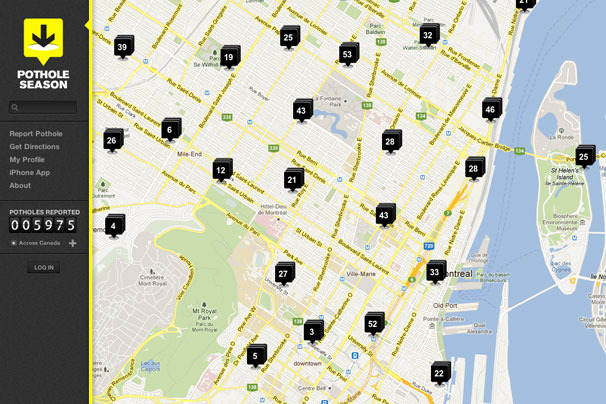
\includegraphics[width=\textwidth]{2-nozioni-preliminari/Immagini/potholes_service.jpg}
	\caption{Potholes Service}\label{fig:potholes}
\end{figure}

L'esempio in Figura \ref{fig:potholes} mostra un simpatico esempio di mashup che posiziona nella mappa le buche stradali segnalate dagli utenti presenti a Montreal in Canada, fornendo anche la possibilit� di calcolare un itinerario per evitarle o almeno trovarne il meno possibile \footnote{Articolo con altri esempi: \url{http://www.pcworld.com/article/252243/top_10_cool_and_useful_google_maps_mashups.html}}. 

Con lo sviluppo dei social network e delle piattaforme di condivisione di contenuti multimediali, i mashup hanno assunto grande importanza perch� � stato possibile creare nuove applicazioni utilizzando i metadati associati ai contenuti, arricchendo di informazioni il contenuto originale.
La diffusione dei mashup � presente anche in domini pi� critici, soprattutto per la facilit� di creazione e la possibilit� di essere utilizzati anche da utenti non esperti in ambito IT, di cui un esempio possono essere gli \emph{enterprise mashups}.
La crescita esponenziale della quantit� di informazioni presente nel web, con i Big Data e il moltiplicarsi dei Web Service, ha portato i mashup ad elemento fondamentale nella creazione delle applicazioni, per via della possibilit� di filtrare i dati necessari all'utente finale e quindi rendere la visione di una parte significativa della moltitudine di informazioni provenienti dai servizi.

%Tra le diverse tipologie di mashups elencate in \cite{picozziTesiDottorato}, per quanto riguarda il progetto CAMUS, ci si soffermer� principalmente sui \emph{mobile mashups}.

\subsection{Classificazione dei mashup\label{sec:mashup-classification}}
I mashup possono essere distinti in diverse tipologie, a prescindere dalla piattaforma sulla quale vengono utilizzati.
In questo caso, la classificazione � basata soprattutto alla metodologia con la quale vengono integrate le diverse risorse che compongono i mashup. Vengono definite tre macro famiglie:
\begin{enumerate}
	\item \textbf{Consumer Mashups} Sono i mashup che combinano elementi visuali e dati da diverse fonti. Un ottimo esempio pu� essere considerato Housing Maps citato nella Sezione \ref{sec:mashup}, dove vengono integrati i dati provenienti da Craigslist e mostrati sulla mappa creata sfruttando le API di Google Maps
	\item \textbf{Data Mashups} Sono mashup che combinano pi� risorse di dati in una singola. Questa tipologia di mashup viene invece sfruttata per realizzare molte applicazioni, anche in settori di utilizzo diversi tra loro.
	Nell'ambito dei viaggi, un esempio viene fornito da Kayak \footnote{Kayak : \url{http://www.kayak.com}}, che � un sito di ricerca dei viaggi che acquisisce dati da oltre 100 siti diversi. Inoltre non vende direttamente i contenuti ai fornitori, ma si propone come un portale attraverso il quale i clienti possono essere dirottati verso le agenzie viaggi per completare la procedura di acquisto o specificare alcune esigenze particolari.
	Un altro ambito completamente differente riguarda Facile.it \footnote{Facile.it : \url{http://www.facile.it}}, che permette di confrontare diverse offerte per quanto riguarda diversi settori (es.: assicurazioni, mutui, linee telefoniche, ecc.), permettendo di visualizzarli in unico portale e valutare la proposta migliore per le esigenze dell'utente
	\item \textbf{Business Mashups} I business mashups sono utili per quanto riguarda l'integrazione di servizi business, permettendo di sviluppare pi� facilmente servizi integrati e, di conseguenza, semplificare l'utilizzo all'utente attraverso interfacce web. Si differiscono dai \emph{consumer mashup} a livello di integrazione con i sistemi business, perch� sono necessarie funzionalit� aggiuntive, riguardanti sicurezza, controllo di accesso, governance e complessit� degli editor utilizzati. Un'altra differenza � data dall'utilizzo crescente di business mashups nei modelli software as a service (SaaS), dove un produttore sviluppa e gestisce un'applicazione web che mette a disposizione dei propri clienti via internet, come servizio cloud.
\end{enumerate}

\subsection{Mobile Mashup\label{sec:mobile-mashup}}

In questi ultimi anni si � avuto un incremento esponenziale del numero di dispositivi mobili, al punto che il loro numero ha superato quello dei personal computer \cite{10.1109/ICSC.2008.100}. Come spiegato nel Global Internet Report di Internet Society\footnote{Global Internet Report 2015: \url{http://www.internetsociety.org/globalinternetreport/assets/download/IS_web.pdf}}, lo sviluppo di nuove applicazioni e sistemi operativi di facile utilizzo, oltre all'incremento della velocit� delle reti mobili (3G e 4G), ha portato a una diffusione capillare dei dispositivi mobili, oltre alla possibilit� di integrare nuovi aspetti finora non utilizzabili facilmente tramite i pc. Un chiaro esempio � dato dalla possibilit� di poter sfruttare la posizione corrente del dispositivo, oppure gli altoparlanti o l'accelerometro.
Questa maggiore integrazione con le esigenze dell'utente ha dato una spinta nella ricerca di come i mashup possano trarre vantaggio da queste nuove opportunit�.
I mobile mashups sono l'applicazione dei mashup web ai mobile devices, pensati come applicazioni native che integrano dati provenienti da servizi differenti \cite{Cappiello2013}. 
Spesso i mashup di questo tipo sono costruiti utilizzando un'applicazione di \emph{Visual Mapping}, dove in modo intuitivo � possibile associare i servizi ai diversi campi da visualizzare nello schermo del device.
In CAMUS � stato adottato l'esempio in \cite{Cappiello:2015:UAE:2788341.2735632}, che pone al centro l'interfaccia utente per integrare i dati, dove durante la creazione delle view dell'applicazione � possibile vedere quasi istantaneamente il risultato del visual mapping. In questo approccio si sono volute seguire le linee dettate dalla filosofia di Model-Driven Engineering (MDE) \cite{schmidt2006model}, che permettono di generalizzare la creazione degli schemi dell'applicazione, e delegare l'interpretazione nelle differenti piattaforme. Cos� � possibile creare applicazioni \emph{cross platform}, cio� che funzionano su diversi sistemi operativi. 

\subsection{Funzionamento generale\label{sec:mashup-operations}}
Generalmente un mashup si compone di due differenti partecipanti, spesso separati fisicamente:
\begin{enumerate}
	\item \textbf{Content Providers} Questi sono i fornitori dei contenuti che verranno utilizzati nell'applicazione di mashup, spesso dei pi� disparati generi e tipi e controllati da differenti tipi.
	Le risorse dalle quali � possibile ottenere contenuti sono:
	\begin{itemize}
		\item \textbf{API} fornite da alcuni provider di contenuti (es. Google, Facebook, Twitter, Amazon)\\
		Una API permette al creazione permette di creare un mashup basato sul web fornendo un mezzo per avere accesso ad una applicazione o a un contenuto (es.: Google Maps), solo per un software compatibile.
		Le API possono essere di due tipi:
		\begin{enumerate}
			\item \emph{Proprietarie} dove � richiesta la stipulazione di un contratto di licenza che comprende spesso il pagamento di una quota per poter usufruire del servizio
			\item \emph{Free} che non richiedono il pagamento di nessuna quota, soltanto, talvolta, � limitato il numero di chiamate che l'applicazione finale pu� fare verso il provider
		\end{enumerate} 
		\item \textbf{Information Feed} Gli Information Feed sono informazioni formattate secondo specifiche prestabilite, spesso utilizzate per distribuire notizie in tempo reale. Un esempio possono essere i news feed in formato RSS che sono utilizzati dalle agenzie di stampa come Reuters\footnote{Reuters: \url{http://it.reuters.com/}} o Ansa\footnote{Ansa: \url{http://www.ansa.it/}} per inviare le notizie alle altre testate giornalistiche
		\item \textbf{Documenti XML/JSON} I formati XML e JSON sono due standard per il trasferimento di dati attraverso Internet. Dopo averli analizzati, gli utenti possono creare dei mashup a partire dai dati generati dai siti web. Questo tipo di operazione � detta \emph{scraping}, e, a differenza di API e Information Feed, � necessaria una conoscenza approfondita dei linguaggi di programmazione e, inoltre, ad ogni variazione nello schema dei dati nel sito web originale, il codice scritto per lo scraping pu� non essere pi� valido
	\end{itemize} 
	\item \textbf{Sito Mashup}
	Il sito del mashup indica dove l'applicazione viene caricata. Questa viene spesso generata utilizzando codice di tipo client-side, cio� che viene eseguito sul client, (es.: JavaScript), con tecnologie di caricamento dei dati dinamiche come Ajax, che permette di evitare di ricaricare l'intera pagina se una parte di essa subisce delle modifiche. Non � tuttavia escluso l'utilizzo di codice server-side
\end{enumerate}

Le informazioni grezze ottenute direttamente dai servizi esterni non � detto che siano gi� pronte per essere visualizzate all'utente finale. Esse necessitano di trasformazioni per poter migliorare e integrare i diversi dati ricevuti. Come esposto in \cite{caio2011tesi} queste operazioni possono essere fatte mediante template visuali, i quali mostrano una rappresentazione dei dati come saranno mostrati nell'applicazione finale. Nel caso di applicazioni sui contenuti si hanno generalmente due schermate: una mostra tutti i risultati provenienti dai diversi servizi, l'altra invece mostra i dettagli dell'elemento selezionato. Le operazioni sui dati da svolgere sono due:

\begin{enumerate}
	\item \textbf{Union} L'operazione di union mostra tutti gli elementi che provengono dai diversi servizi, specificando soltanto una piccola parte dei dati complessivi ritornati, cercando di trovare le similitudini e quindi aggregare le risposte che si riferiscono allo stesso elemento
	\item \textbf{Merge} L'operazione di merge permette di mostrare tutti i dettagli dell'istanza selezionata. In questo modo i dati provenienti da pi� servizi vengono mostrati nella stessa schermata. Questa operazione � definita durante la composizione del mashup, quando vengono associati i campi al servizio corrispondente
\end{enumerate}

\begin{figure}[h]
	\centering
	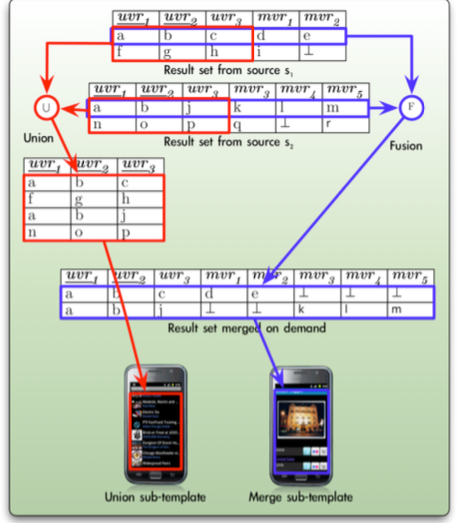
\includegraphics[width=0.5\textwidth]{2-nozioni-preliminari/Immagini/merge-union.png}
	\caption{Esempio merge e union}\label{fig:merge-union}
\end{figure}

\section{Web Services\label{sec:web-services}}

Per \emph{Web Service} si intendono tutti quei software che vengono utilizzati per favorire la comunicazione tra diverse macchine. Secondo la definizione formale fornita dal Consorzio W3C\footnote{Consorzio W3C: \url{https://www.w3.org/}} \virgolette{un Web Service � un sistema software creato allo scopo di permettere la comunicazione tra macchine attraverso un network. \upe composto da un'interfaccia descritta in un linguaggio interpretabile dalle macchine (WSDL in particolare). [...]} \cite{world2004web}. In questa definizione viene citato l'utilizzo del protocollo SOAP: in realt�, qualche anno pi� tardi, la definizione � stata estesa \cite{w3c2004web}, includendo nell'elenco:

\begin{itemize}
	\item \emph{REST Web Services}, dove l'obiettivo principale � la manipolazione di \emph{risorse} utilizzando operazioni che non necessitano di mantenere uno stato
	\item \emph{Servizi Web Arbitrari}, dove � possibile esporre a piacimento un insieme di operazioni
\end{itemize}

Il motivo principale che ha spinto verso questa scelta � da ricercare nella definizione stessa di \emph{web service}: l'obiettivo principale � quello di permettere lo scambio di informazioni tra macchine, favorendo l'interoperabilit� tra sistemi e linguaggi di programmazione differenti. La maggior parte dei servizi utilizza il protocollo HTTP come livello di trasporto: questa scelta ha l'enorme vantaggio di poter sfruttare lo stesso protocollo gi� utilizzato per le comunicazioni via internet, cos� da ridurre i costi di gestione necessari per la messa in opera di un diverso protocollo. Nel corso del tempo sono nate diverse tipologie di servizi: alcuni, come SOAP, forniscono una struttura standardizzata da seguire per l'implementazione dei servizi compatibili mentre altri, come REST, forniscono delle linee guida sulla metodologia da seguire per l'implementazione del servizio, ma non sono dipendenti da nessuna tecnologia in particolare. La creazione di servizi che adempiono ad uno specifico compito ha favorito un ulteriore aspetto: la composizione. \upe possibile creare dei servizi che ne sfruttano contemporaneamente diversi al fine di realizzare un processo pi� complesso \cite{weerawarana2005web}. Recentemente questo concetto � stato ulteriormente esteso con la realizzazione dei cosiddetti \emph{mashup} \cite{benslimane2008services}, applicazioni web che permettono di combinare assieme informazioni provenienti da diverse fonti dinamicamente, in modo da fornire un'esperienza utente migliore.

Di seguito vengono analizzate alcune tra le tecnologie e paradigmi pi� utilizzati per la creazione di servizi, tra cui SOAP, REST e GraphQL.

\subsection{SOAP}

\upe l'acronimo di \emph{Simple Object Access Protocol} e fornisce un framework per lo scambio di messaggi.  Utilizza come formato di risposta XML e nella maggior parte dei casi si appoggia al protocollo HTTP come livello di trasporto. Vengono scambiate delle \emph{buste}, che contengono le informazioni come interrogare il servizio e come sono rappresentate le risposte. L'architettura SOAP viene distinta per tre caratteristiche principali:

\begin{enumerate}
	\item \textbf{Estensibilit�} Le funzionalit� di base possono essere ampliate attraverso l'utilizzo di estensioni
	\item \textbf{Neutralit�} Non dipende da nessun protocollo di comunicazione in particolare. Quello pi� utilizzato � HTTP, ma esistono delle implementazioni per SMTP, TCP, UDP o JMS per citarne alcuni
	\item \textbf{Indipendenza} Pu� essere utilizzato da diversi linguaggi di programmazione
\end{enumerate}

In seguito, SOAP � stato utilizzato come base per altre tecnologie legate ai web services, come il \emph{Web Services Description Language} (WSDL), che � un'interfaccia di descrizione delle funzionalit� fornite dal servizio, e l'\emph{Universal Description Discovery and Integration} (UDDI), che � un registro dove � possibile ricercare i servizi.

\subsection{REST}

\upe l'acronimo di \emph{REpresentational State Transfer} ed � uno stile architetturale che definisce determinati vincoli di comportamento per componenti, connettori e dati che compongono un sistema distribuito ipermediale. \emph{REST} � prima di tutto un paradigma: non vengono infatti menzionati n� i dettagli relativi all'implementazione dei componenti n� i protocolli da utilizzare proprio per concentrarsi sul ruolo dei componenti, sulle loro interazioni e come interpretare le informazioni. Il termine \emph{REpresentational State Transfer} � stato utilizzato per la prima volta nella tesi di dottorato di Roy Fielding \cite{fielding2000architectural}. \emph{REST} viene largamente utilizzato per descrivere i servizi web, in modo tale da non generare contraddizioni durante l'implementazione. I sistemi che rispettano i principi \emph{REST} vengono chiamati \emph{RESTful}. Nella maggior parte dei casi, i sistemi \emph{RESTful} comunicano attraverso i verbi standard del protocollo HTTP (GET, POST, PUT, DELETE, ecc.). Utilizza le \emph{web resources} come interfaccia per comunicare con i sistemi esterni, identificate tramite un \emph{Uniform Resource Identifier} (URI). L'applicazione delle linee guida definite dall'architettura permette di ottenere i seguenti vantaggi: performance, scalabilit�, semplicit�, manutenibilit�, visibilit�, portabilit� ed affidabilit�.

I vincoli definiti dall'architettura sono:

\begin{itemize}
	\item \textbf{Client-server} C'� una separazione delle attivit� che devono essere eseguite sul client e sul server. Per esempio, i client non devono occuparsi della memorizzazione dei dati, che rimane interna al server, in modo da favorire la \emph{portabilit�} del codice del client. Il server invece non deve preoccuparsi dell'interfaccia e dello stato dell'utente, in modo da rendere l'implementazione del server pi� semplice e \emph{scalabile}. Il client e il server possono essere sostituiti e sviluppati separatamente a patto che le interfacce tra di loro rimangono immutate
	\item \textbf{Stateless} Lo stato non deve essere assolutamente salvato sul server. Ogni richieste che proviene dal client deve contenere tutte le informazioni necessarie alla sua esecuzione. Sar� compito del client mantenere memorizzato lo stato corrente. Lo stato della sessione pu� per� essere trasferito dal server verso un ulteriore servizio di memorizzazione, per esempio un database, per un periodo di tempo limitato. Al client viene affidato il compito di decidere quando � pronto a passare ad un nuovo stato
	\item \textbf{Cacheable} Sia il client sia il server possono effettuare caching delle risposte. Le risposte devono innanzitutto definire se possono essere salvate in cache o meno, in modo da limitare le situazioni nelle quali il client utilizza informazioni non corrette o non pi� valide. Implementare un ottimo sistema di cache permette di ridurre il numero di interazioni tra il client e il server, migliorando la scalabilit� e le performance del sistema
	\item \textbf{Layered system} Un client non pu� specificare se � connesso direttamente al server di pi� basso livello oppure ad un server intermediario. L'utilizzo di server intermediari permette di migliorare la scalabilit� del sistema, tramite load balancer e cache distribuite. Possono inoltre fornire ulteriori misure di sicurezza
	\item \textbf{Uniform interface} L'utilizzo delle \emph{uniform interface} permette di semplificare e disaccoppiare i vari componenti dell'architettura, rendendo possibile lo sviluppo indipendente delle varie parti del sistema. I quattro vincoli riguardo le \emph{uniform interface} sono:
	\begin{enumerate}
		\item \textbf{Identificazione delle risorse} Le singole risorse vengono identificate nella richiesta tramite, per esempio, un \emph{URI}. Le risorse sono concettualmente separate dalle rappresentazioni che vengono inviate al client. Per esempio, un server pu� inviare dati acquisiti dal database sotto forma di file HTML, XML o JSON, che sono diversi dalla rappresentazione interna del server
		\item \textbf{Manipolazione delle risorse tramite le rappresentazioni} Ogni rappresentazione di una risorsa che viene inviata al client deve contenere tutte le informazioni che permettano la modifica o l'eliminazione della risorsa
		\item \textbf{Messaggi autoesplicativi} Ogni messaggio deve contenere informazioni su come trattare l'informazioni che porta con s�, tramite per esempio i \emph{media type}
		\item \textbf{Sfruttamento dell'hypermedia (HATEOAS)} I client possono effettuare delle azioni che vengono dinamicamente messe a disposizione dal server tramite hypermedia (es.: link). Ad eccezione dello stato iniziale, il client conosce le attivit� che possono essere eseguite a partire da una data rappresentazione solamente tra quelle che espone
	\end{enumerate}
\end{itemize}

Applicando i principi REST alle API dei servizi web si ottengono quelle che vengono definite \emph{RESTful API}. Le \emph{RESTful API} che sfruttano il protocollo HTTP sono definite tramite le seguenti caratteristiche:

\begin{itemize}
	\item Possiedono un URI di base
	\item Definiscono un media type, che indica il formato della risposta, che nelle implementazioni pi� comuni � JSON
	\item Utilizzano i verbi standard del protocollo HTTP (es.: OPTIONS, GET, PUT, POST e DELETE)
	\item Mettono a disposizione dei link come referenza per passare alle risorse correlate
	\item Utilizzano dei link come referenza dello stato
\end{itemize}

Solitamente ad una URI pu� essere associata una funzione diversa in base al verbo con la quale viene chiamata, come si pu� notare nell'esempio in Tabella \ref{table:esempio-rest-api}.

\begin{table}[h]
	\caption{Esempio RESTful API}
	\label{table:esempio-rest-api}
	\noindent\makebox[\textwidth]{%
	\begin{tabularx}{1.3\textwidth}{lXXXX}
		\toprule
		\thead{Risorsa} & \thead{GET} & \thead{PUT} & \thead{POST} & \thead{DELETE} \\
		\midrule
		\url{http://api.example.com/resources/} & \textbf{Elenca} le URI insieme ad eventuali altri dettagli sulla collezione & \textbf{Sostituisce} la collezione con un'altra & \textbf{Aggiunge} un nuovo elemento alla collezione. L'URI viene generato automaticamente e restituito dall'operazione & \textbf{Elimina} l'intera collezione \\
		\hline
		\url{http://api.example.com/resources/item17} & \textbf{Restituisce} una rappresentazione dell'oggetto, espresso con un particolare \emph{media type} & \textbf{Sostituisce} l'elemento della collezione o, se non esiste, ne crea uno nuovo & \textbf{Crea} un nuovo elemento & \textbf{Rimuove} l'elemento dalla collezione \\
		\bottomrule
	\end{tabularx}}
\end{table}

\subsection{GraphQL}

\emph{GraphQL}\footnote{GraphQL: \url{http://graphql.org/}} �, come suggeriscono le ultime due lettere del nome, un \emph{query language}, creato come supporto alla realizzazione di applicazioni client, che mette a disposizione una sintassi intuitiva e flessibile ed un sistema che permette al client di specificare i requisiti e le interazioni sui dati \cite{website:graphql-specs}. Rispetto all'approccio REST, \emph{GraphQL} permette di effettuare richieste pi� efficienti dei dati ed evita la duplicazione della logica lato server che pu� verificarsi nel caso di endpoint personalizzati. Una delle principali differenze rispetto a REST riguarda la possibilit� di lasciare al client la scelta dei dati da ricevere. Questa modifica nasce dall'idea che � il client a conoscere nel dettaglio quali dati servono per comporre la view e quindi gli viene delegata la responsabilit� di richiedere solo quelli essenziali all'interno della query.

Alla base di \emph{GraphQL} ci sono i seguenti principi:

\begin{itemize}
	\item \textbf{Gerarchico} Una buona parte dei prodotti sviluppati implica la creazione e manipolazione di view gerarchiche. Per mantenere coerenza con la struttura delle applicazioni, le query \emph{GraphQL} sono esse stesse strutturate gerarchicamente. La query viene plasmata esattamente come i dati che deve restituire. \upe un metodo naturale per permettere ai client di descrivere i vincoli sui dati
	\item \textbf{Basato sul prodotto} \emph{GraphQL} � stato creato tenendo ben presenti i requisiti delle view e del come gli sviluppatori di front-end li esplicitano
	\item \textbf{Tipizzato} Ogni server \emph{GraphQL} definisce il proprio schema specifico per l'applicazione in uso. Le query vengono eseguite a partire dal contesto definito da questo schema. Inoltre vengono effettuati dei controlli al fine di verificare che la query sia sintatticamente corretta e valida  prima di essere eseguita
	\item \textbf{Query definite dal client} Negli schemi viene inoltre definito il formato della risposta, compresa la tipologia di ogni dato. Sar� poi il client a specificare esattamente quali sono le informazioni che gli interessano. Rispetto ad altri approcci, dove � il server a decidere quali dati restituire ai client, in \emph{GraphQL} invece vengono restituiti solamente i dati che vengono richiesti e nulla di pi�
	\item \textbf{Introspettivo} Qualsiasi schema \emph{GraphQL} pu� essere interrogato tramite query. In questo modo � possibile conoscere la struttura globale dello schema, cos� come le query che sono permesse e quali dati possono essere richiesti. Queste introspezioni vengono utilizzate da vari tool per avere una visione completa dello schema che viene esposto dal server
\end{itemize}

\begin{center}
	\begin{minipage}[t]{0.5\textwidth}
		\begin{lstlisting}[caption=Esempio di query GraphQL, label=lst:esempio-query-graphql]
{
	!user!(@id@: ~2~) {
		!name!
		!surname!
	}
}
		\end{lstlisting}
	\end{minipage}%
	\hspace{5mm}%
	\begin{minipage}[t]{0.4\textwidth}
		\begin{lstlisting}[caption=Esempio di risposta, label=lst:esempio-risposta-graphql, style=json]
{
	"user": {
		"name": "Mario",
		"surname": "Rossi"
	}
}
		\end{lstlisting}
	\end{minipage}	
\end{center}

Nel Blocco \ref{lst:esempio-query-graphql} viene riportato un semplice esempio di query scritta tramite \emph{GraphQL}. Con questa query si vogliono acquisire i dati relativi all'utente con identificativo 2, ed in particolare si � interessati a ricevere il suo \emph{nome} e \emph{cognome}. Nel Blocco \ref{lst:esempio-risposta-graphql} viene invece mostrato un esempio di risposta che viene ricevuta dalla server.

\emph{GraphQL} fornisce inoltre un'altra funzionalit� estremamente utile: le \emph{connessioni}. Una \emph{connessione} permette ad un oggetto di definire i legami che ha con altri oggetti, anche di tipo diverso dal proprio. In questo modo � possibile richiedere direttamente le informazioni riguardo altri oggetti tramite un'unica query; questa caratteristica non � presente nei sistemi REST e permette di ottenere un netto miglioramento delle performance. Infatti nei sistemi REST, per richiedere le rappresentazioni correlate sono necessarie \emph{n} query, dove \emph{n} � il numero di risorse da richiedere. Con GraphQL invece � sufficiente una sola richiesta, nella quale viene specificato che si � interessati anche alle altre risorse. Inoltre, GraphQL mette a disposizione per ogni connessione la \emph{paginazione} dei risultati, ossia la possibilit� di richiedere un determinato numero di elementi ad ogni richiesta. Ad ogni oggetto viene automaticamente associato un \emph{token} che lo identifica univocamente: in questo modo � possibile chiedere ulteriori elementi in una seconda query, specificando il \emph{token} dell'oggetto dal quale si desidera partire.

\begin{center}
	\hspace*{-1.5cm}
	\begin{minipage}[t]{0.63\textwidth}
		\begin{lstlisting}[caption=Esempio di connessione GraphQL, label=lst:esempio-connessione-graphql]
{
	!user! (@id@: ~4802170~) {
		!id!
		!name!
		!isViewerFriend!
		!profilePicture! (@size@: ~50~) {
			!uri!
			!width!
			!height!
		}
		!friendConnection!(@first@: ~2~) {
			!totalCount!
			!friends!: {
				!id!
				!name!
			}
		}
	}
}
		\end{lstlisting}
	\end{minipage}%
	\begin{minipage}[t]{0.63\textwidth}
		\begin{lstlisting}[caption=Esempio di risposta, label=lst:esempio-risposta-connessione-graphql,style=json]
{
	"user": {
		"id": 4802170,
		"name": "Lee Byron",
		"isViewerFriend": true,
		"profilePicture": {
			"uri": "cdn://pic/4802170/50",
			"width": 50,
			"height": 50
		},
		"friendConnection": {
			"totalCount": 13,
			"friends": [
				{
					"id": 305249,
					"name": "Stephen Schwink"
				},
				{
					"id": 3108935,
					"name": "Nathaniel Roman"
				}
			]
		}
	}
}
		\end{lstlisting}
	\end{minipage}	
\end{center}

Nel Blocco \ref{lst:esempio-connessione-graphql} viene mostrata una query pi� complessa della precedente. La \emph{connessione} viene definita da \virgolette{friendConnection}, che viene utilizzata per recuperare gli amici dell'utente corrente. Si vuole far notare che gli oggetti che vengono restituiti nel campo \virgolette{friends} sono dello stesso tipo dell'utente richiesto in origine: questo vuol dire che � possibile produrre infiniti livelli gerarchici. Se, all'interno di un utente amico, si specifica di nuovo la connessione \virgolette{friendConnection}, verranno restituiti anche gli amici di quello specifico utente. Altro punto interessante, come citato in precedenza, delle \emph{connessioni} riguarda la possibilit� di richiedere solo un sottoinsieme dei risultati: nell'esempio vengono richiesti solamente i primi due amici dell'utente. Come si pu� notare nel Blocco \ref{lst:esempio-risposta-connessione-graphql}, vengono restituiti solamente i primi due amici, nonostante il campo \virgolette{totalCount} indichi che l'utente ha in totale 13 amici. Tramite ulteriori query possono essere richiesti gli altri amici dell'utente.

\textcolor{red}{Aggiungere parte sulle mutations?}

\section{Stato dell'arte\label{sec:stato-arte}}

\textcolor{red}{work in progress}

In questa sezione vengono presentati ...

\subsection*{Swagger}

Per descrizione servizi (STEFANO)

Swagger \footnote{Swagger: \url{http://swagger.io}} � uno dei servizi pi� potenti per la definizione di interfacce REST per i servizi.
Lo scopo di Swagger � di definire un'interfaccia standard e indipendente dal linguaggio a diverse REST API per permettere sia umani che macchine di scoprire e capire le risorse di un servizio senza accedere ai suoi parametri tecnici, come codice sorgente, documentazione o ispezionando il traffico di rete. Una volta definiti i servizi via Swagger, un consumatore pu� interagire con il servizio remoto con una minima parte di logica implementativa.
Swagger � quindi, tecnicamente parlando, una specificazione formale supportata da un grande ecosistema di strumenti aggiuntivi, comprendendo interfacce utente front-end, librerie di codice a basso livello e soluzioni commerciali per gestire le API.
Per poter descrivere la propria API con swagger ci sono diversi approcci disponibili:
\begin{itemize}
	\item \textbf{Top-down} Si pu� usare un approccio di tipo top-down quando si vuole usare lo \emph{Swagger Editor} \textcolor{red}{(Immagine o reference)} per creare la definizione del servizio e successivamente generare l'applicazione server con lo strumento \emph{Swagger Codegen}
	\item \textbf{Bottom-up} Nel caso in cui si ha una API REST gi� esistente e si vuole creare una nuova definizione si usa un approccio bottom-up. \upe possibile creare la definizione manualmente utilizzando lo \emph{Swagger Editor} oppure, nel caso di utilizzo di uno dei framework supportati (es.: JAX-RS, node.js, ecc.), � possibile generare in modo automatico la definizione Swagger
\end{itemize}

Nel caso in cui si sia utilizzatori di API e si vuole integrare una API che gi� possiede una definizione Swagger, si pu� utilizzare la versione online della \emph{Swagger UI} per esplorarla e successivamente lo \emph{Swagger Codegen} per generare la libreria client desiderata.

\textcolor{red}{migliorare con esempi}
\subsection*{Appery.io}

Per visual composition (VALERIO)

Appery.io � un sito web che ha due funzionalit� principali: la costruzione di applicazioni mobile in maniera rapida e l'offerta di un servizio di Mobile Backend as a service (MBaaS).
Con il servizio di App Builder, � possibile creare applicazioni per dispositivi mobili che possono girare sui sistemi operativi pi� diffusi come iOS, Android e Windows Phone, a partire da un unica implementazione logica.
\upe possibile creare applicazioni di due tipi: 
\begin{enumerate}
	\item \textbf{Hybrid Apps} Creare applicazioni ibride che utilizzano API comuni e che girano in modo consistente su iOS, Android e Windows Phone, con il supporto integrato per framework diffusi come Apache Cordova (precedentemente conosciuto come PhoneGap), Ionic e jQuery Mobile. In questo modo � possibile fornire all'applicazione le potenzialit� delle applicazioni completamente native, senza avere la complessit� di imparare diversi linguaggi nativi. Inoltre � possibile integrare diversi plug-in di terze parti per questi framework
	\item \textbf{Responsive Web Apps}
	Con il supporto a Bootstrap, il framework UI per le interfacce di tipo responsive, � possibile creare applicazioni web che sono utilizzabili su tutti i tipi di dispositivi e dimensioni dello schermo
\end{enumerate}

Per poter creare le applicazioni si utilizzano paradigmi di \emph{Visual Development} per permettere di creare rapidamente e in modo intuitivo nuove applicazioni, semplicemente usando \emph{drag and drop}. \upe possibile utilizzare template preinstallati oppure crearne uno nuovo e i dati provenienti dai servizi possono essere associati utilizzando l'editor di Visual Data Mapping, anche scrivendo frammenti di codice personalizzati per garantire la massima adattabilit� alle esigenze dell'utente.
\begin{itemize}
	
	\item \textbf{Sviluppo}
	La costruzione delle applicazioni � svolta in modo modulare, con componenti riutilizzabili in maniera veloce e semplice. Possono essere gi� presenti oppure creati da zero. Il tipo di struttura dati utilizzato, invece, � di tipo model-based, in particolare si � usato il pattern MVC (Model View Controller). Anche per quanto riguarda lo storage dei dati la soluzione scelta � di tipo visuale, con la Storage API, che permette di gestire le variabili.
	\item \textbf{Deployment} Successivamente alla fase di sviluppo, in Appery.io � presente anche una parte per poter esportare la propria applicazione nelle diverse piattaforme. In particolare, il metodo pi� veloce per poter diffondere l'app appena creata � l'utilizzo di un QR code, quindi � sufficiente inviare questo codice per far scaricare l'applicazione sul dispositivo. Oltre a questo metodo � possibile esportare l'applicazione, come sorgenti HTML5/CSS oppure come progetti per le IDE di sviluppo native come Android Studio, xCode o Visual Studio
	\item \textbf{Testing} \upe considerato anche l'aspetto del testing, sia per quanto riguarda HTML5 che le app native.
	Nel primo caso � possibile eseguire testing istantaneamente sul browser o direttamente sul telefono, mentre nel secondo caso � supportato anche l'offline testing, vale a dire che � possibile capire se l'applicazione pu� essere eseguita su un dispositivo senza installarla direttamente su di esso.
	\item \textbf{Administration} La parte amministrativa � la parte di Mobile Backend as a Service, perch� permette di gestire tutta la parte di logica e storage sul cloud. Per quanto riguarda questo aspetto � presente in Appery.io una console di controllo, con la quale � possibile inviare notifiche push, controllare i certificati e le API key necessarie alla app, condividere lo sviluppo con altri utenti, gestire i ruoli del team di sviluppo e controllare i rilasci delle versioni dell'applicazione.
\end{itemize}
 


\subsection*{Kimono}

Per integrazione servizi (STEFANO)

\subsection*{Peudom}

Per composizione mashup  (VALERIO)



\subsection*{AdAPT}

Controllare ... (STEFANO)




\chapter{Il Progetto CAMUS\label{ch:camus}}

In questo capitolo ...

\section{Panoramica del progetto}

CAMUS � l'acronimo di Context-Aware Mobile mashUpS e, come si pu� intuire dal nome, il principale obiettivo del progetto � quello di proporre un framework per la realizzazione di mashup mobile che sfruttano il contesto nel quale si trova l'utente. Vengono dunque sfruttati due ambiti di ricerca differenti, cio� la gestione del \emph{contesto} e i \emph{mashup}, in quanto l'unione delle loro potenzialit� pu� aiutare a fornire un'esperienza utente migliore. Infatti la quantit� di servizi e dati disponibili online rende difficoltoso il processo di selezione delle informazioni che realmente sono rilevanti per colui/e che deve usufruirne. Questo problema � proprio il punto in cui CAMUS vuole proporsi come soluzione; utilizza il \emph{contesto} per raccogliere informazioni sul profilo e gli interessi dell'utente e sull'ambiente nel quale si trova, al fine di selezionare i servizi pi� idonei alla situazione e filtrare le informazioni che sono di maggior interesse. Inoltre sfrutta la dinamicit� di presentazione che caratterizza i mashup per adattare il modo nel quale queste informazioni vengono mostrate e la flessibilit� di integrare dati aggiuntivi provenienti da diverse fonti.

In particolare, viene applicato il concetto dei mashup al mondo mobile: il risultato finale consiste in un'app per smartphone o tablet che adatta il proprio aspetto in base a delle regole di visualizzazione. Questa caratteristica permette di ottenere un'estrema flessibilit�, in quanto non � necessario rilasciare nuove app ogni volta che si vuole effettuare un cambio di aspetto. Fornisce inoltre la libert� di variare spesso l'interfaccia grafica in modo che si adatti a diverse situazioni di utilizzo.

CAMUS prevede l'integrazione di alcune \emph{web app}, ognuna delle quali deve permettere la realizzazione intuitiva della rappresentazione del contesto e dell'interfaccia grafica assunta dall'app. Le web app principali sono due: \emph{i)} la prima coinvolge la realizzazione del \emph{contesto}, che viene rappresentato tramite un modello che si presta molto bene alla visualizzazione grafica; \emph{ii)} la seconda riguarda la composizione degli elementi che formano l'interfaccia grafica della mobile app.

Gli altri componenti principali del framework sono il \emph{server} e la \emph{mobile app}. Il \emph{server} � il cuore del sistema e orchestra la comunicazione tra gli altri componenti. Il suo compito primario � quello di fornire le informazioni idonee all'app mobile, a partire dal contesto che quest'ultima gli invia. La \emph{mobile app} infine contiene il motore di rendering che interpreta le regole definite sul come mostrare i componenti e li disegna in moda da essere fruibili dall'utente.

\section{Obiettivi del progetto\label{sec:obiettivi-progetto}}

L'obiettivo principale del progetto CAMUS � definire la metodologia con la quale � possibile creare app sfruttando i mashup ed il contesto, al fine di mostrare all'utente le informazioni che sono pi� pertinenti alla situazione nella quale si trova.

Per la creazione del framework sono state rispettate le seguenti linee guida:

\begin{itemize}
	\item \textbf{Creazione visuale} Questo punto � relativo alla modalit� di realizzazione delle app. Si vuole ideare un sistema che permetta la composizione dell'interfaccia grafica interamente in modo visuale, senza la necessit� di scrivere linee di codice
	\item \textbf{Contestualit�} Si vuole sfruttare il contesto dell'utente per comprendere quali siano le sue esigenze e mostrargli cos� le informazioni che sono pi� pertinenti alla situazione. In questo modo � possibile utilizzare anche diverse fonti per acquisire dati pi� precisi e variegati, che poi verranno filtrati adeguatamente in modo da selezionare unicamente le informazioni pi� rilevanti e nascondere quelle che porterebbero solamente ad una maggior confusione
	\item \textbf{Semplicit�} Ogni operazione deve essere facile, in modo che anche persone non pratiche di informatica possano creare delle app CAMUS. Qualsiasi attivit� di creazione e modifica viene dunque effettuata tramite un'interfaccia grafica, in modo che l'utente venga guidato nello svolgere i compiti. Inoltre sono stati scelti dei modelli concettuali semplici, in modo che siano intuitivi a chiunque ma che allo stesso tempo siano abbastanza potenti per creare schemi di una certa complessit�
	\item \textbf{Automazione} Si vuole far ripetere all'utente il minor numero di azioni; in quest'ottica vengono sfruttati i sensori disponibili sui dispositivi per acquisire in maniera automatica alcuni dati, sgravando l'utente da questo compito
	\item \textbf{Uniformit�??} Il framework non prevede l'interfacciamento con un database per il recupero delle informazioni, bens� si � scelto di acquisire tutti i dati necessari tramite \emph{servizi}. Questa soluzione rende pi� flessibile l'accesso ai dati, in quanto viene fornita un'interfaccia comune per servizi sia interni, cio� gestiti direttamente dal creatore dell'app, sia esterni, cio� mantenuti da terzi. Inoltre apre la strada per l'utilizzo dei servizi di supporto, che forniscono dati complementari in modo da arricchire il dataset finale
\end{itemize}

\section{Integrazione del contesto con i mashup}

\textcolor{red}{"Limiti" delle due aree\\
	dire come mai sono complementari, come possono essere unite e i vantaggi che porta\\
	specificare la divisione tra gestione dati, che viene demandata soprattutto al contesto, e gestione interfacce, che viene data ai mashup\\
	dire anche perch� si � tolta la parte di gestione dati dai mashup}

\section{Utilizzo dei servizi}

Uno dei punti chiave del framework, seguendo la filosofia dei mashup, � di non essere limitati ad una singola fonte per l'acquisizione dei dati, bens� si vuole essere in grado di recuperare le informazioni da diverse sorgenti. In questo modo � possibile ottenere diversi vantaggi, come l'acquisizione di una maggiore quantit� di risultati, ottenere informazioni pi� complete, ecc. Presenta per� anche degli svantaggi: avere molti dati a disposizione pu� essere dispersivo ed esiste il rischio di ottenere entit� duplicate. Per fornire un'elevata flessibilit� il framework prevede il disaccoppiamento della logica di accesso ai dati: per l'acquisizione le informazioni viene fornita un'unica interfaccia, rappresentata dai \emph{servizi}. Questo metodo permette di avere una descrizione unica sul come recuperare i dati, indipendentemente dal fornitore che li mette a disposizione. L'utilizzo dei servizi porta i seguenti vantaggi:

\begin{itemize}
	\item \textbf{Variet�}	L'utilizzo di un'interfaccia generica per l'accesso ai dati favorisce l'acquisizione di informazioni da fonti diverse. In questo modo � possibile ottenere dei dataset pi� ampi
	\item \textbf{Integrabilit�} Ogni servizio restituisce i dati secondo una propria rappresentazione. Avere un unico metodo di accesso ai dati permette anche di descrivere come queste informazioni vengono trattate una volta ricevute. Questo passaggio permette di uniformare le rappresentazioni fornite in ingresso tale per cui vengano trasformate in un'altra rappresentazione che sia utile per il trattamento e l'elaborazione di questi dati
	\item \textbf{Completezza} Acquisendo informazioni da diverse fonti � possibile ottenere degli elementi duplicati. Questa caratteristica potrebbe sembrare un difetto mentre in realt� fornisce una risorsa molto importante: la possibilit� di ottenere degli elementi pi� completi. Diverse fonti possono essere utilizzate per acquisire informazioni di entit� diversa, in modo da generare un elemento descritto in maniera pi� precisa e che colga maggiori aspetti
\end{itemize}

Questa scelta permette inoltre di dividere l'acquisizione dei dati in due passaggi: \emph{i)} acquisizione delle informazioni principali; \emph{ii)} acquisizione di dati che vanno ad arricchire le informazioni principali. L'astrazione dei servizi come metodo per ottenere i dati permette di utilizzare lo stesso formalismo per entrambe le attivit�.

\section{Caso di studio del turismo\label{sec:caso-studio-turismo}}

Al fine di pensare a come specificare il progetto CAMUS, � stato necessario introdurre un caso di studio che fosse sufficientemente attinente al nostro progetto.
La scelta � caduta sull'agenzia viaggi, un ambito di tipo turistico, perch� pu� nascere la necessit� di avere un sistema di mashup che fornisca dati di diversa natura al viaggiatore, a seconda del contesto nel quale si trova.
Le due figure principali in questo caso di studio sono l'agente di viaggio e il viaggiatore. L'agente ha il compito di organizzare tutto il tour, con tutte le prenotazioni, spostamenti principali e soggiorni per il viaggiatore, mentre il viaggiatore � colui che fisicamente compie il viaggio, quindi lo possiamo considerare come l'utente finale.
Quest'ultimo, oltre ad essere gi� in possesso delle prenotazioni per mezzi di trasporto, pernottamento ed eventuali extra di soggiorno, pu� avere la necessit� di ottenere informazioni aggiuntive.
Con la grande quantit� di informazioni e risorse presenti sul Web, non � sempre vero che l'utente abbia una maggiore conoscenza, anzi, alcune volte, si ottiene l'effetto contrario, in quanto non � in grado di filtrare le informazioni per le sue esigenze. Data la grande diffusione di dispositivi mobili, si � scelto di introdurre questo sistema mobile context-aware e in questo modo poter offrire questa nuova esperienza d'uso per il cliente. Per mezzo della web app del sistema, l'agente di viaggio pu� configurare per il viaggiatore un'applicazione personalizzata, la quale � in grado di adattarsi alle diverse condizioni di utilizzo dell'utente. La dinamicit� dell'applicazione � dettata dal cambiamento dei servizi invocati dal sistema a seconda delle variazioni nel contesto.
Ad esempio, a Milano nell'ora di cena, se l'utente seleziona come argomento di interesse i ristoranti ed � senza automobile, saranno invocati servizi adatti ad offrire questo tipo di risultati all'utente, con i dovuti mezzi di trasporto locale. Se il viaggiatore si spostasse verso Torino, l'applicazione invocherebbe servizi diversi per fornire dei dati migliori all'utente.
Questa definizione ed associazione dei dati viene fatta dall'agente di viaggio,il quale si suppone che abbia una certa esperienza nel saper scegliere quali servizi sono pi� attinenti a un certo elemento dell'albero di contesto, da cui il sistema, con operazioni spiegate nel Capitolo \ref{ch:metodologia}, sceglie quali servizi invocare dinamicamente.



\chapter{Metodologia di lavoro\label{ch:metodologia}}


In questo capitolo viene presentata la metodologia seguita per il design e la creazione delle applicazioni CAMUS, utilizzando un approccio di Visual Programming dei mashup \cite{DBLP:journals/tweb/CappielloMP15}. \upe stato scelto di mettere l'utente finale al centro della progettazione, tenendo conto delle sue esigenze di utilizzo e cercando di mascherare la complessit� delle operazioni. %Esempio Viaggio???%
Nelle sezioni successive verranno esposti i problemi che sono stati incontrati e le conseguenti scelte progettuali, fino ad arrivare all'architettura realizzata nell'implementazione del prototipo.

\section{Modello del contesto\label{sec:modello-contesto}}

Come illustrato nella Sezione \ref{sec:context-awareness}, esistono diversi modelli per rappresentare il contesto. Ai fini del progetto si � resa necessaria la scelta di un modello che soddisfi le seguenti caratteristiche:

\begin{itemize}
	\item Permetta di rappresentare informazioni \emph{predefinite} e \emph{parametriche}, dove per \emph{predefinite} si intendono le caratteristiche del contesto che vengono specificate a priori, mentre per \emph{parametriche} si intendono i dati che devono essere specificati dall'utente in quanto non � possibile (e conveniente) enumerarli. Un esempio di \emph{informazione predefinita} � descritta dalla \virgolette{Tipologia di Viaggio}, che pu� assumere i valori \virgolette{Avventuroso}, \virgolette{Rilassante}, \virgolette{Lavoro}, ecc.; un esempio di \emph{informazione parametrica} � la localit�, dove bisogna specificare le coordinate geografiche in cui si trova l'utente
	\item Deve consentire una rappresentazione gerarchica. Ad esempio, \emph{Mezzi di trasporto pubblici} si pu� specializzare in bus, treno, car sharing, ecc.
	\item Deve essere facilmente personalizzabile ed adattarsi a diversi ambiti di utilizzo. Per esempio, deve essere in grado di descrivere il contesto che pu� assumere un'app per la gestione dei viaggi come un'app per la gestione del personale, dove alcuni possibili contesti possono essere definiti dal \emph{ruolo} che ricopre un dipendente e, nel caso in cui sia necessario recarsi da un cliente, i dati relativi ai clienti nella zona in cui si trova
	\item Deve possedere una rappresentazione visiva semplice e chiara, in modo che sia utilizzabile anche da persone non esperte di informatica
\end{itemize}

Tra i diversi modelli a disposizione, si � ritenuto che il \emph{Context Dimension Tree (CDT)} sia il modello che rispetti maggiormente le richieste precedentemente elencate.

Oltre alla classificazione dei nodi originale del CDT, viene aggiunta un'ulteriore divisione in base al ruolo che un nodo pu� assumere durante la fase di selezione dei servizi:

\begin{itemize}
	\item \textbf{Nodo filtro} \upe la tipologia predefinita. I nodi di tipo filtro permettono, come si pu� dedurre dal nome, di filtrare i servizi che sono idonei all'utilizzo in un determinato contesto
	\item \textbf{Nodo ranking} Questa tipologia viene assegnata ad alcuni nodi specifici, come ad esempio quello relativo alla \emph{localit�}, che assumono una maggiore importanza durante la selezione dei servizi, in quanto permettono di scegliere dei servizi che hanno un maggior impatto nel contesto specifico. Nell'esempio relativo alla \emph{localit�}, permettono di dare una maggiore rilevanza ai servizi che sono pi� attinenti al luogo e che quindi forniscono delle informazioni pi� accurate
\end{itemize}

\section{Creazione dell'ecosistema dei servizi\label{sec:ecosistema-servizi}}

I servizi rappresentano un punto cardine del sistema, in quanto mettono a disposizione le risorse che verranno mostrate all'utente. Si � deciso di dividere i servizi in due categorie ben distinte, in base alla funzionalit� del servizio:

\begin{enumerate}
	\item \textbf{Primari} Sono i servizi che vengono interrogati in prima istanza per acquisire le informazioni di interesse relative al contesto nel quale si trova l'utente. Per esempio, se si effettua la ricerca di un ristorante, le informazioni principali saranno il nome del ristorante, l'indirizzo e il numero di telefono. TripAdvisor\footnote{\url{https://www.tripadvisor.it/}} e Zomato\footnote{\url{https://www.zomato.com/it}} sono due esempi di servizi primari
	\item \textbf{Supporto} Sono i servizi che vengono utilizzati per arricchire le informazioni acquisite tramite i servizi primari. Possono mettere a disposizione dati aggiuntivi, contenuti multimediali (es.: foto e video) oppure possono fornire un'integrazione con altre app presenti sul dispositivo. Alcuni esempi di servizi di supporto sono le informazioni sul meteo, la cartina geografica del luogo o le indicazioni dei mezzi di trasporto per raggiungere il posto. Invece l'apertura del dialer telefonico quando viene selezionato il numero di telefono o l'utilizzo dell'app di navigazione preferita quando si sceglie un indirizzo rappresentano degli esempi di integrazione con altre app
\end{enumerate}

Per quanto queste categorie rappresentino una divisione molto precisa dei servizi, non vengono considerate come rigide. Come gi� evidenziato in \cite{rizzo2015progettazione}, ogni servizio espone una o pi� operazioni, e non � detto che tutte rientrino nella medesima categoria. Pu� capitare che un servizio metta a disposizione un'operazione che viene considerata primaria ed un'altra che invece fornisce informazioni di supporto. Si � deciso quindi di non effettuare una categorizzazione a livello di servizio, bens� per ogni operazione, in modo da garantire una maggiore flessibilit�.

Per coerenza, d'ora in avanti verr� utilizzata la nomenclatura \emph{operazione primaria} per riferirsi alle operazioni che forniscono le informazioni principali e \emph{operazione di supporto} per le operazioni che arricchiscono le informazioni primarie.

Per l'acquisizione dei dati � importante che il server sappia come interrogare i servizi e come interpretare le risposte. Si � deciso dunque di creare una repository con tutti i servizi che possono essere utilizzati dal sistema. Questa repository � composta dai \emph{descrittori dei servizi}, che contengono le informazioni necessarie per la gestione dei servizi. Ogni descrittore � composto da una prima parte comune relativa alle informazioni del servizio (es.: nome, categoria, url base, ecc.) e da una parte specifica, costituita dall'elenco delle operazioni che espone. Ogni operazione rappresenta l'unit� principale di ogni servizio, in quanto fornisce le seguenti informazioni che permettono di effettuare le richieste:

\begin{itemize}
	\item \textbf{Elenco dei parametri} Per interrogare un servizio � necessario comporre una query con i dati che si vogliono richiedere. Queste informazioni sono dipendenti dalla specifica implementazione del servizio e variano tra un servizio e l'altro. Nel descrittore vengono dunque elencati i parametri necessari per la composizione della query e dove andare a recuperare i relativi valori. L'acquisizione dei valori pu� avvenire secondo tre differenti modalit�:
	\begin{enumerate}
		\item \emph{Default} Il valore viene impostato direttamente nel descrittore (es.: l'API key per l'autenticazione)
		\item \emph{Mapping CDT} Viene definita l'associazione con uno o pi� nodi del CDT e il valore viene recuperato in base alla selezione effettuata dall'utente (es.: le coordinate geografiche). Questi valori possono essere eventualmente trasformati da quelli simbolici del contesto ad un'altra rappresentazione adatta per effettuare la query (es.: dal valore \virgolette{Restaurant} del contesto viene associata la tipologia \virgolette{food})
		\item \emph{Mapping Term} Questa modalit� viene utilizzata esclusivamente per i servizi di supporto e fornisce un placeholder nelle query che verr� rimpiazzato a runtime con il valore reale acquisito dalla risposta o dal dispositivo
	\end{enumerate}
	\item \textbf{Schema della risposta} Per ottenere omogeneit� tra le risposte ottenute dai diversi servizi, i dati ricevuti devono essere trasformati secondo uno schema comprensibile dalla mobile app. Per effettuare questa trasformazione vengono in aiuto i \emph{termini} (es.: titolo, indirizzo, descrizione, ecc.), che rappresentano le classi semantiche di appartenenza degli attributi. L'elenco dei termini disponibili viene mantenuto in una repository come per i descrittori dei servizi. Queste annotazioni hanno una duplice utilit�: in primo luogo, definendo il significato semantico di ogni attributo, semplificano l'integrazione dei dati provenienti da diversi servizi, in secondo luogo semplificano la creazione dei mashup, come verr� approfonditamente trattato nella Sezione \ref{sec:mashup-design}, in quanto permettono di ragionare su categorie astratte di dati rispetto a dati reali forniti dai vari servizi e agevolano la riusabilit� degli schemi in diversi contesti 
	\item \textbf{Gestione della paginazione} I dati che vengono restituiti a seguito di una query possono essere molteplici. Per semplificare la gestione delle risposte, i servizi implementano delle politiche di paginazione, dove vengono specificati il numero di risultati che si vogliono ottenere in una pagina e un numero che indica la pagina che � stata richiesta \cite{masse2011rest}. Questa sezione serve appositamente per indicare quali sono i parametri che vengono utilizzati dal servizio per richiamare le diverse pagine che compongono i risultati
\end{itemize}

\section{Associazione dei servizi al CDT\label{sec:associazione-servizi-cdt}}

Una volta che i servizi sono stati aggiunti alla repository � necessario specificare le associazioni che permettono la selezione dei servizi in base al contesto nel quale si trova l'utente.

Nel modello originale del CDT, presentato nella Sezione \ref{sec:context-dimension-model}, il processo di selezione dei dati rilevanti per un determinato contesto avveniva tramite la definizione di viste, che venivano create in linguaggio SQL e associate ai \emph{nodi valore}. Come evidenziato anche nella precedente ricerca \cite{rizzo2015progettazione}, questa metodologia non � pi� applicabile principalmente per due motivi:

\begin{enumerate}
	\item Si vuole rendere il funzionamento del sistema il pi� semplice possibile per essere utilizzato da persone che non hanno profonde conoscenze di informatica, e la scrittura di query in SQL non � alla portata di chiunque
	\item Non avendo a disposizione direttamente i dati, bens� i servizi da invocare per acquisirli, la selezione tramite viste non � la pi� idonea ad essere utilizzata
\end{enumerate}

Volendo mantenere un approccio che sia semplice e allo stesso tempo funzionale, si � deciso di associare le operazioni definite dai singoli servizi ai nodi dell'albero di contesto. 

\begin{figure}[h]
	\centering
	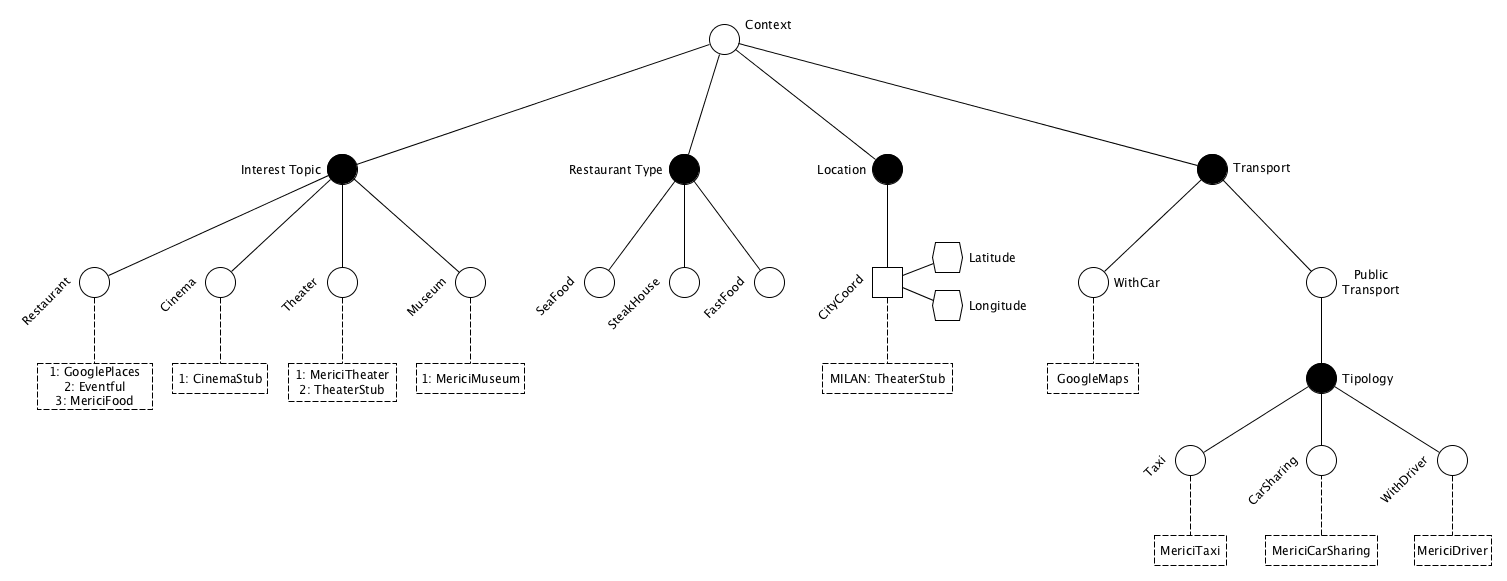
\includegraphics[width=\textwidth]{4-metodologia/Immagini/associazioni-cdt.png}
	\caption{Associazione dei servizi al CDT}\label{fig:associazione-servizi-cdt}
\end{figure}

Come si pu� notare dalla Figura \ref{fig:associazione-servizi-cdt}, le operazioni vengono associate ai nodi di tipo \virgolette{valore} o \virgolette{attributo}. Nel primo caso l'operazione viene aggiunta all'elenco di operazioni che ogni nodo definisce, nel secondo caso � necessario associare a quale/i valore/i associare l'operazione (es.: per il campo \virgolette{Citt�} bisogna definire il nome della citt�, invece per l'attributo \virgolette{Coordinate} � necessario specificare la latitudine e longitudine del luogo). Generalmente le associazioni vengono effettuate nei nodi foglia; tuttavia � possibile effettuare delle associazioni anche nei nodi che hanno dei figli, quando per esempio un servizio copre diverse categorie e non ha senso che sia scelto in una sola di esse.

Per quanto riguarda le \emph{operazioni primarie}, quando vengono associate ad un determinato contesto viene definito anche un indice di \emph{priorit�}: questo valore � un numero intero, a partire da 1 e crescente all'interno del singolo nodo, definisce l'importanza che il servizio assume in quel determinato contesto e verr� utilizzato nella fase di selezione dei servizi illustrata nel Capitolo \ref{sec:primary-service-selection}. Questo indicatore ha senso di essere utilizzato esclusivamente nei \emph{nodi valore}, in quanto contengono una raccolta generica di servizi, mentre per i \emph{nodi attributo} non � necessario, poich� l'ordinamento all'interno di una categoria di attributi non � sempre univoca. Se si prende per esempio un elenco di servizi associati ad una citt� tramite le sue coordinate geografiche, si pu� considerare come indice di priorit� la lontananza rispetto all'utente, che pu� essere calcolata solamente a runtime e pu� variare spesso.

Una menzione particolare viene riservata all'associazione con la dimensione \emph{Interest Topic}. Come precedentemente esposto nella Sezione \ref{sec:modello-contesto}, il modello del contesto deve essere in grado di adattarsi a diversi ambiti di utilizzo. Gli \emph{Interest Topic} fungono proprio da descrittori delle situazioni principali nelle quali l'utente pu� trovarsi. Un contesto specifico pu� essere molto complesso: gli \emph{Interest Topic} hanno il vantaggio di permettere la definizione di una categoria di riferimento, sulla quale poi specializzare la ricerca secondo le altre caratteristiche del contesto attive. Alcuni esempi di \emph{Interest Topic} sono i \virgolette{Ristoranti}, gli \virgolette{Hotel}, i \virgolette{Musei}, ecc.
Al fine di far rispettare questa classificazione � stato introdotto il vincolo che ogni \emph{operazione primaria} deve obbligatoriamente essere aggiunta ad almeno un \emph{Interest Topic}. Non viene imposto un vincolo sul numero di \emph{Interest Topic} differenti ai quali pu� essere associata un'operazione, in quanto pu� essere valida per ambiti differenti.

Per le \emph{operazioni di supporto} non � sempre necessario definire le associazioni con i nodi del CDT. Alcuni operazioni di supporto possono essere richiamate in modo statico quando non necessitano del contesto per essere scelte (es.: i servizi generici come Wikipedia\footnote{\url{https://en.wikipedia.org/wiki/Main_Page}} o Flickr\footnote{\url{https://www.flickr.com/}}). Per altre operazioni, come per esempio quelle relative ai mezzi di trasporto, � invece necessario basarsi sul contesto per selezionare la pi� idonea alla situazione. Per esempio, se un utente specifica che non dispone di un'auto e che si trova a Milano, allora il sistema proporr� i mezzi di trasporto pubblici presenti nella citt�, insieme all'elenco di altre tipologie di trasporto come i taxi o il car sharing. In questo caso � dunque necessario, come nel caso delle operazioni primarie, definire le associazioni delle operazioni con i nodi del CDT. Il processo di associazione � simile a quello delle operazioni primarie, la principale differenza risiede nel fatto che non bisogna specificare la priorit� dei servizi, mentre le altre assunzioni rimangono valide.

\section{CDT su misura per gli utenti\label{sec:cdt-su-misura}}

Il modello del CDT definito nella Sezione \ref{sec:associazione-servizi-cdt} viene chiamato \emph{CDT Universale}, in quanto rappresenta lo schema pi� completo del quale il sistema dispone. Questo CDT deve descrivere tutti i possibili contesti che si vogliono gestire; possono coesistere diversi ambiti in parallelo, con le relative dimensioni che vanno a specializzare il dominio generale. Com'� facilmente intuibile, questo schema pu� diventare di enormi dimensioni, rendendolo di fatto inutilizzabile per via della moltitudine di selezioni possibili. Inoltre emerge il problema dei \emph{contesti non validi}, cio� quei contesti che non possono esistere nella realt�. Per esempio, scegliere come \emph{Interest Topic} la ricerca di \virgolette{Ristoranti} e selezionare di voler fare un viaggio \virgolette{Rilassante} non � un contesto valido, in quanto la dimensione \virgolette{Tipologia di Viaggio} ha senso di essere attivata solo quando viene selezionato come \emph{Interest Topic} quello relativo ai viaggi. Queste due problematiche vanno in senso contrario con i principi di usabilit� e semplicit� che sono stati presi come linee guida per il progetto.

Una prima soluzione consiste nell'introdurre l'elenco delle \emph{dimensioni consentite} per ogni \emph{Interest Topic}. In questo modo, nella fase di scelta delle dimensioni che si vogliono attivare, l'interfaccia grafica pu� essere aggiornata in seguito ad ogni selezione, mostrando solamente le dimensioni che � possibile scegliere senza generare conflitti. In questo modo si risolverebbero entrambi i problemi sopra citati, in quanto l'elenco delle \emph{dimensioni consentite} permette di ridurre il numero totale di contesti generabili e impedisce la selezione di dimensioni che porterebbero ad effettuare delle selezioni erronee.

Per quanto questa soluzione sia tecnicamente valida, rimane aperta un'ulteriore questione: all'utente potrebbero venire proposte comunque una serie di opzioni che non sono di suo interesse. Per esempio, un utente deve pianificare un viaggio e non possiede animali e nel CDT viene definita una dimensione \virgolette{Con Animali Domestici}, per specificare che bisogna cercare strutture che ammettano l'accesso anche agli animali. In questa situazione verrebbe ogni volta proposta la selezione del possesso animali all'utente, mentre potrebbe essere sempre omessa in quanto non utile nella descrizione del contesto di quello specifico utente.

Per risolvere questa ulteriore problematica, relativa pi� al profilo specifico di ogni utente, si � pensato di far entrare in gioco la figura dell'\emph{esperto di settore}: l'esperto � la persona alla quale si deve rivolgere l'utente per ottenere una personalizzazione dell'app. Come verr� descritto nella sezione \ref{sec:mashup-design}, l'esperto di settore � colui che ha il compito di adattare l'aspetto della mobile app, andando a  modificare lo schema di mashup. Si � deciso dunque che si tratta della figura pi� indicata anche per adattare il contesto al profilo specifico di ogni utente. Nasce quindi l'idea di creare dei CDT specifici per gli utenti, che mostrano solamente le dimensioni che sono di loro interesse. Questi CDT vengono definiti come \emph{CDT su misura} o \emph{Tailored CDT}. In pratica, all'esperto di settore viene dato in carico il compito di \emph{eliminare} le dimensioni che non sono utili all'utente e che creerebbero solamente confusione. Questi alberi di contesto vengono creati a partire dallo schema globale e modificati dall'\emph{esperto di settore} appositamente per uno specifico utente. Oltre alla possibilit� di eliminare le dimensioni del contesto non necessarie, viene data anche la libert� di effettuare ulteriori modifiche per migliorare l'esperienza dell'utente:

\begin{itemize}
	\item Viene data la possibilit� di impostare dei valori predefiniti. Questa caratteristica � sempre correlata con il profilo dell'utente e da un certo punto di vista � un problema simile a quello esposto in precedenza riguardo le dimensioni non interessanti. In questo caso per�, invece che rimuovere totalmente un ramo dell'albero, viene assegnato un valore che rimane sempre valido. Questa caratteristica � molto importante, ed � utile che coesista insieme alla possibilit� di rimuovere le dimensioni non interessanti. Si prenda per esempio un utente che non dispone di un proprio mezzo di trasporto: in questo caso non si pu� rimuovere completamente la dimensione che riguarda i \emph{Trasporti}, in quanto all'utente pu� sempre interessare come muoversi con i mezzi pubblici. \upe invece pi� conveniente fissare il valore \virgolette{Trasporto Pubblico} per segnalare che l'utente utilizzer� sempre i mezzi di trasporto pubblici per raggiungere i luoghi di suo interesse
	\item \upe possibile inoltre modificare le associazioni delle operazioni con i nodi del CDT, comprese, solo per le \emph{operazioni primarie}, le priorit� che assumono all'interno di ogni nodo. Questa funzionalit� tende a sfruttare in maniera pi� marcata le conoscenze dell'\emph{esperto di settore} per migliorare la qualit� dei risultati ottenuti dal sistema. Pu� essere utilizzata per diversi scopi, come favorire l'uso di determinati servizi rispetto ad altri o sostituire alcuni servizi che in una certa localit� non sono disponibili o non forniscono dei buoni risultati.
\end{itemize}

\section{Selezione delle operazioni in base al contesto\label{sec:selezione-operazioni}}

Nelle precedenti sezioni � stato spiegato come � possibile aggiungere nuovi servizi nel sistema, come i servizi vengono associati al contesto ed infine come � possibile personalizzare il contesto in base alle preferenze dei singoli utenti.

Resta da definire il metodo col quale a runtime questi servizi vengono selezionati. Questa fase � una tra le pi� importanti all'interno di CAMUS, in quanto la selezione dei servizi da utilizzare impatta in maniera preponderante nella qualit� e rilevanza dei dati che verranno mostrati all'utente. \upe necessario quindi definire un algoritmo che tenga conto della situazione nella quale si trova l'utente e a partire da questa selezioni le operazioni pi� idonee a soddisfare la richiesta. Come gi� evidenziato nella Sezione \ref{sec:associazione-servizi-cdt}, le associazioni vengono effettuate seguendo due approcci differenti in base alla tipologia dell'operazione, \emph{primaria} oppure di \emph{supporto}. Il motivo principale risiede nel fatto che queste due tipologie di operazione hanno scopi differenti e necessitano dunque di due approcci di selezione appositi. Di seguito vengono analizzati entrambi i metodi utilizzati in CAMUS, concentrandosi su di una tipologia di operazione alla volta.

\subsection*{Operazioni primarie\label{(sec:selezione-op-primarie)}}

Come esposto nella Sezione \ref{sec:associazione-servizi-cdt}, ogni operazione viene associata ad uno o pi� nodi dell'albero di contesto e ad ognuna di queste associazioni viene assegnato un valore che rappresenta la \emph{priorit�} che l'operazione assume all'interno del nodo. Il primo passo per la selezione delle operazioni � l'assegnazione di un \emph{punteggio} ad ogni operazione che ha una o pi� corrispondenze all'interno dell'albero di contesto. Un contesto � un elenco di coppie $ \textless dimensione, valore \textgreater $, che rappresentano i nodi selezionati dall'utente. La selezione dei servizi che hanno validit� nelle singole coppie avviene tramite una ricerca \emph{chiave-valore}, dove la \emph{chiave} � l'etichetta della dimensione mentre il \emph{valore} � il valore specifico assunto dalla dimensione, tra le associazioni definite nell'albero di contesto. Questa ricerca fornisce come risultato un elenco delle operazioni che sono adatte all'utilizzo nello specifico contesto, assieme al relativo valore di priorit�, per ogni associazione trovata. \upe necessario introdurre un ulteriore parametro che influisce nella formula per l'assegnamento del \emph{punteggio} alle operazioni: il \emph{peso} dei nodi. Come definito nella Sezione \ref{sec:modello-contesto}, vengono introdotte due nuove tipologie di nodo: \emph{filtro} e \emph{ranking}. Il \emph{peso} di un nodo viene assegnato in base alla \emph{tipologia} del nodo, rispettando il vincolo:

\begin{equation*}
	w_{FILTRO} < w_{RANKING} \quad \forall\ n \in CDT
\end{equation*}

In pratica, ad ogni nodo \emph{filtro} deve essere assegnato un peso strettamente minore rispetto ad un nodo \emph{ranking}. Il punteggio \emph{R} di ogni operazione \emph{o} viene calcolato tramite la funzione:

\begin{equation}
	R_o = \sum_{i \in SA(o)}{\frac{w_i}{p_i}}
\end{equation}

dove \emph{SA(o)} rappresenta l'insieme delle associazioni trovate per l'operazione \emph{o}, $ w_i $ e $ p_i $ rappresentano rispettivamente il \emph{peso} e il valore di \emph{priorit�} dell \emph{i}-esimo nodo. Una volta calcolati i \emph{punteggi}, l'elenco delle operazioni viene riordinato in modo \emph{decrescente} e vengono selezionati le top-N operazioni. In Figura \ref{fig:esempio-punteggio-primari} viene definito un contesto di esempio con le associazioni delle operazioni primarie ai vari nodi dell'albero.

\begin{figure}[h]
	\centering
	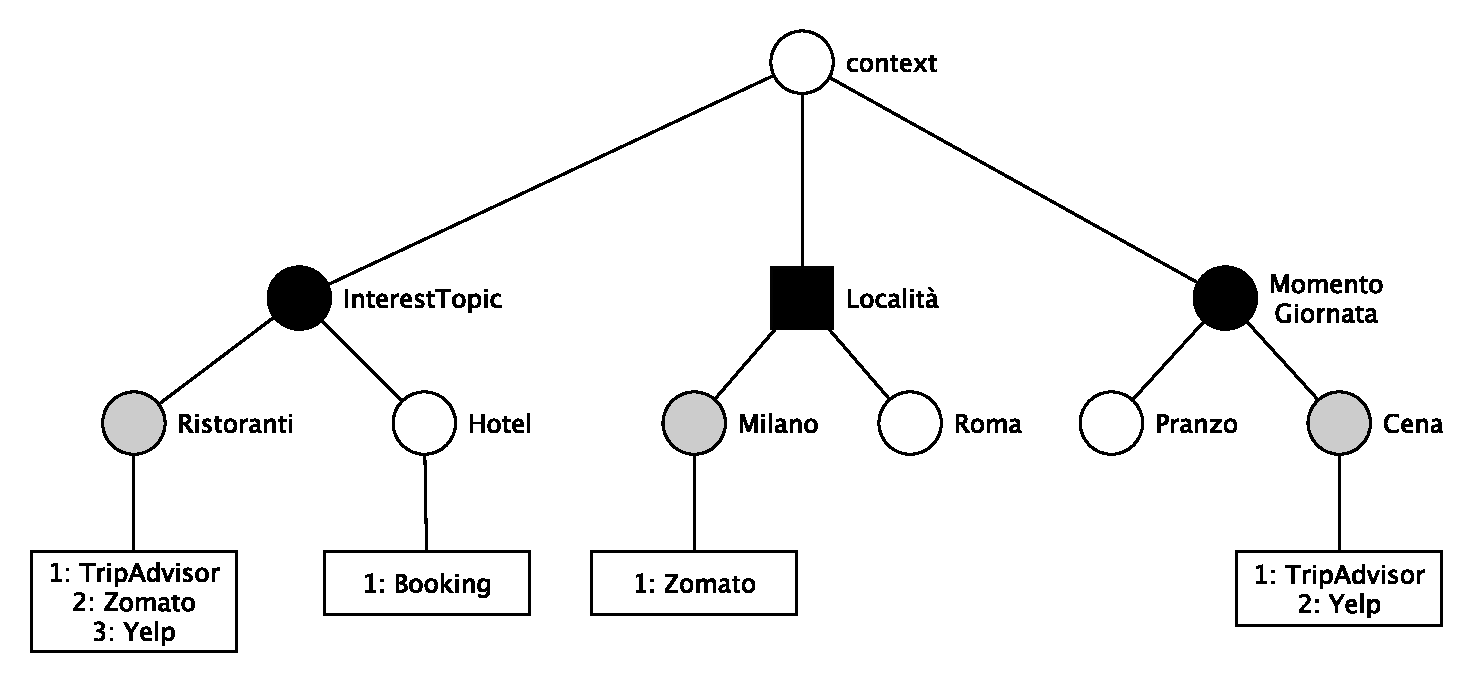
\includegraphics[width=\textwidth]{4-metodologia/Immagini/esempio-punteggio-primari.pdf}
	\caption{Esempio di assegnazione del punteggio per le operazioni primarie}\label{fig:esempio-punteggio-primari}
\end{figure}

I nodi \emph{Interest Topic} e \emph{Momento Giornata} sono di tipo \emph{filtro} mentre il nodo \emph{Localit�} � di tipo \emph{ranking} (come evidenziato dalla diversa forma utilizzata). I nodi foglia di colore grigio sono quelli selezionati, che corrispondono al contesto $ C = InterestTopic: Ristoranti\ \land\ Localit\acute{a}: Milano\ \land\ MomentoGiornata: Cena $. Dalla fase di ricerca vengono selezionate le operazioni dei servizi $ \{TripAdvisor, Zomato, Yelp\} $. Considerando come pesi dei nodi $ w_{FILTER} = 1 $  e $ w_{RANKING} = 4 $, viene calcolato il punteggio per ogni operazione:

\begin{align*}
	R_{TripAdvisor} &= \frac{1}{1} + \frac{1}{1} = 2 \\
	R_{Zomato} &= \frac{1}{2} + \frac{4}{1} = \frac{9}{2} = 4,5\\
	R_{Yelp} &= \frac{1}{3} + \frac{1}{2} = \frac{5}{6} \approx 0,83
\end{align*} 

Riordinando la lista si ottiene $ \{ Zomato, TripAdvisor, Yelp \} $ e scegliendo i top-2 risultati si ottiene la selezione finale $ \{ Zomato, TripAdvisor \} $.

\subsection*{Operazioni di supporto\label{sec:selezione-op-supporto}}

A differenza delle operazioni primarie, per quelle di supporto non viene definito un valore di \emph{priorit�}. Quindi la precedente funzione per il calcolo del punteggio non � pi� applicabile. \upe stata inoltre considerata un'ulteriore problematica per la quale la precedente funzione non � pi� utilizzabile. Per esempio, si consideri un servizio di supporto che fornisce indicazioni sui mezzi di trasporto pubblici. Molti di questi servizi hanno validit� locale, infatti ogni citt� ha il proprio gestore per il servizio di trasporto pubblico. Quindi, nella fase di calcolo del punteggio, anche questi servizi verrebbero considerati e in alcune situazioni erroneamente selezionati come risultato finale. Si � optato per un metodo di selezione pi� rigido rispetto al caso delle operazioni primarie. La prima fase di ricerca tramite \emph{chiave-valore} resta sempre valida e fornisce l'elenco delle operazioni che hanno almeno un'associazione soddisfatta. Di questa lista viene successivamente effettuato il \emph{conteggio} del numero di associazioni totali per ogni operazione. Viene inoltre mantenuto per ogni operazione un valore che indica il numero totale di associazioni con l'albero del contesto. Vengono selezionate solamente le operazioni che rispettano le seguenti regole:

\begin{enumerate}
	\item Il numero di vincoli dell'operazione deve essere pari al conteggio del numero di associazioni
	\item Il numero di associazioni � pari al valore massimo restituito nella fase di ricerca
\end{enumerate}

Quest'ultima restrizione relativa la selezione delle sole operazioni con il massimo numero di vincoli rispettati deriva dal fatto che un maggior numero di vincoli corrisponde ad una maggiore attinenza dell'operazione al contesto. In Figura \ref{fig:esempio-selezione-supporto} viene mostrato un contesto di esempio con le associazioni delle operazioni di supporto ai vari nodi dell'albero.

\begin{figure}[h]
	\centering
	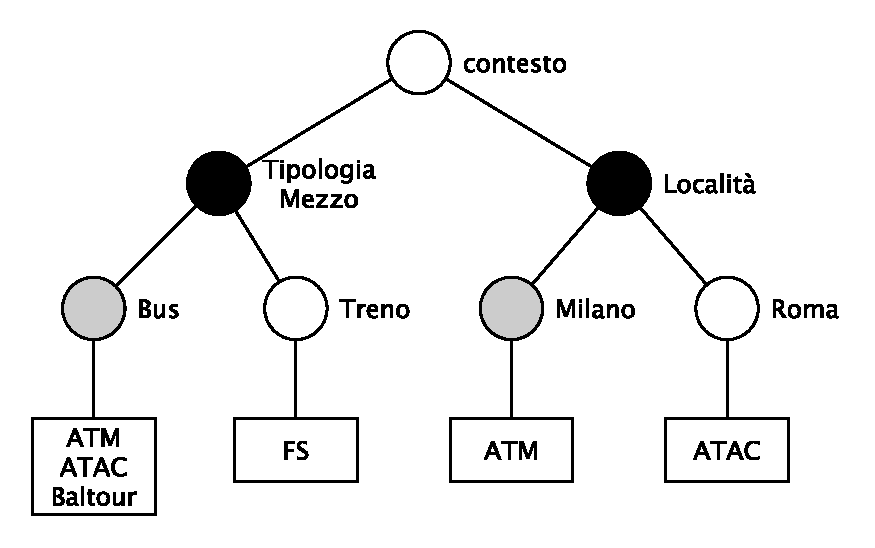
\includegraphics[width=0.5\textwidth]{4-metodologia/Immagini/esempio-selezione-supporto.pdf}
	\caption{Esempio di selezione delle operazioni di supporto}\label{fig:esempio-selezione-supporto}
\end{figure}

I nodi attivi sono evidenziati in grigio ed equivalgono al contesto $ C = TipologiaMezzo: Bus\ \land\ Localit\acute{a}: Milano $. Per le operazioni \emph{ATM} e \emph{ATAC} vengono definiti 2 vincoli, mentre per le operazioni \emph{FS} e \emph{Baltour} viene effettuata una singola associazione. La fase di ricerca restituisce le operazioni \emph{ATM} con conteggio pari a 2 e le operazioni \emph{ATAC} e \emph{Baltour} entrambe con conteggio pari a 1. Applicando la regola \emph{1)} restano valide le operazioni \emph{ATM} e \emph{Baltour}. La regola \emph{2)} porta al risultato finale della selezione del servizio \emph{ATM}. Come si pu� notare, quest'ultima regola permette di selezionare le operazioni che hanno una maggiore rilevanza per il contesto corrente, escludendo le operazioni che forniscono risultati meno precisi.\\

Un'ultima considerazione, che � valida per entrambi i casi precedentemente descritti, riguarda la selezione di un nodo contesto che ha dei figli.

\begin{figure}[h]
	\centering
	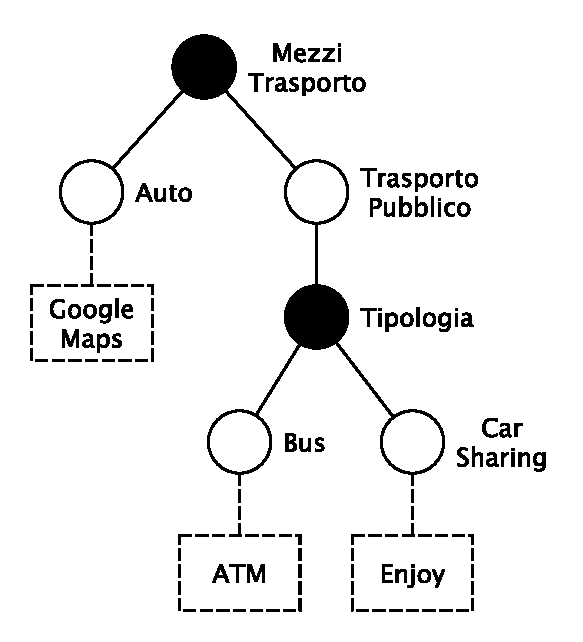
\includegraphics[width=0.4\textwidth]{4-metodologia/Immagini/esempio-gerarchia.pdf}
	\caption{Esempio gerarchia}\label{fig:esempio-gerarchia}
\end{figure}

In Figura \ref{fig:esempio-gerarchia} viene mostrato un esempio di albero gerarchico. Nel caso in cui l'utente scelga un qualsiasi nodo foglia la selezione avviene come nei casi esposti. Invece per il contesto $ C = MezziTrasporto: TrasportoPubblico $ deve essere trattato separatamente, in quanto il valore \emph{Trasporto Pubblico} possiede un nodo figlio. In questo caso la selezione del valore \emph{Trasporto Pubblico} significa che per l'utente � indifferente prendere una tipologia di mezzo piuttosto che un'altra. Il problema che emerge riguarda le associazioni con le operazioni: come si pu� notare nell'esempio, le operazioni vengono associate solamente ai nodi foglia. Quindi il contesto precedente porterebbe alla selezione di nessuna operazione. Per risolvere questo problema viene definito che, quando viene selezionato un nodo che ha dei figli, tutti i suoi discendenti vengono automaticamente selezionati. In pratica, il precedente contesto diventa $ C' = MezziTrasporto: TrasportoPubblico\ \land\ Tipologia: Bus\ \land\ Tipologia: Taxi $. In questo modo la selezione dei servizi ritorna a funzionare correttamente come nei casi descritti precedentemente.

\section{Integrazione dei dati\label{(sec:integrazione-dati)}}

\textcolor{red}{come vengono integrati i dati (algoritmo merge)\\
	rimozione duplicati}

\section{Mashup Design\label{sec:mashup-design}}

\begin{figure}[h]
	\centering
	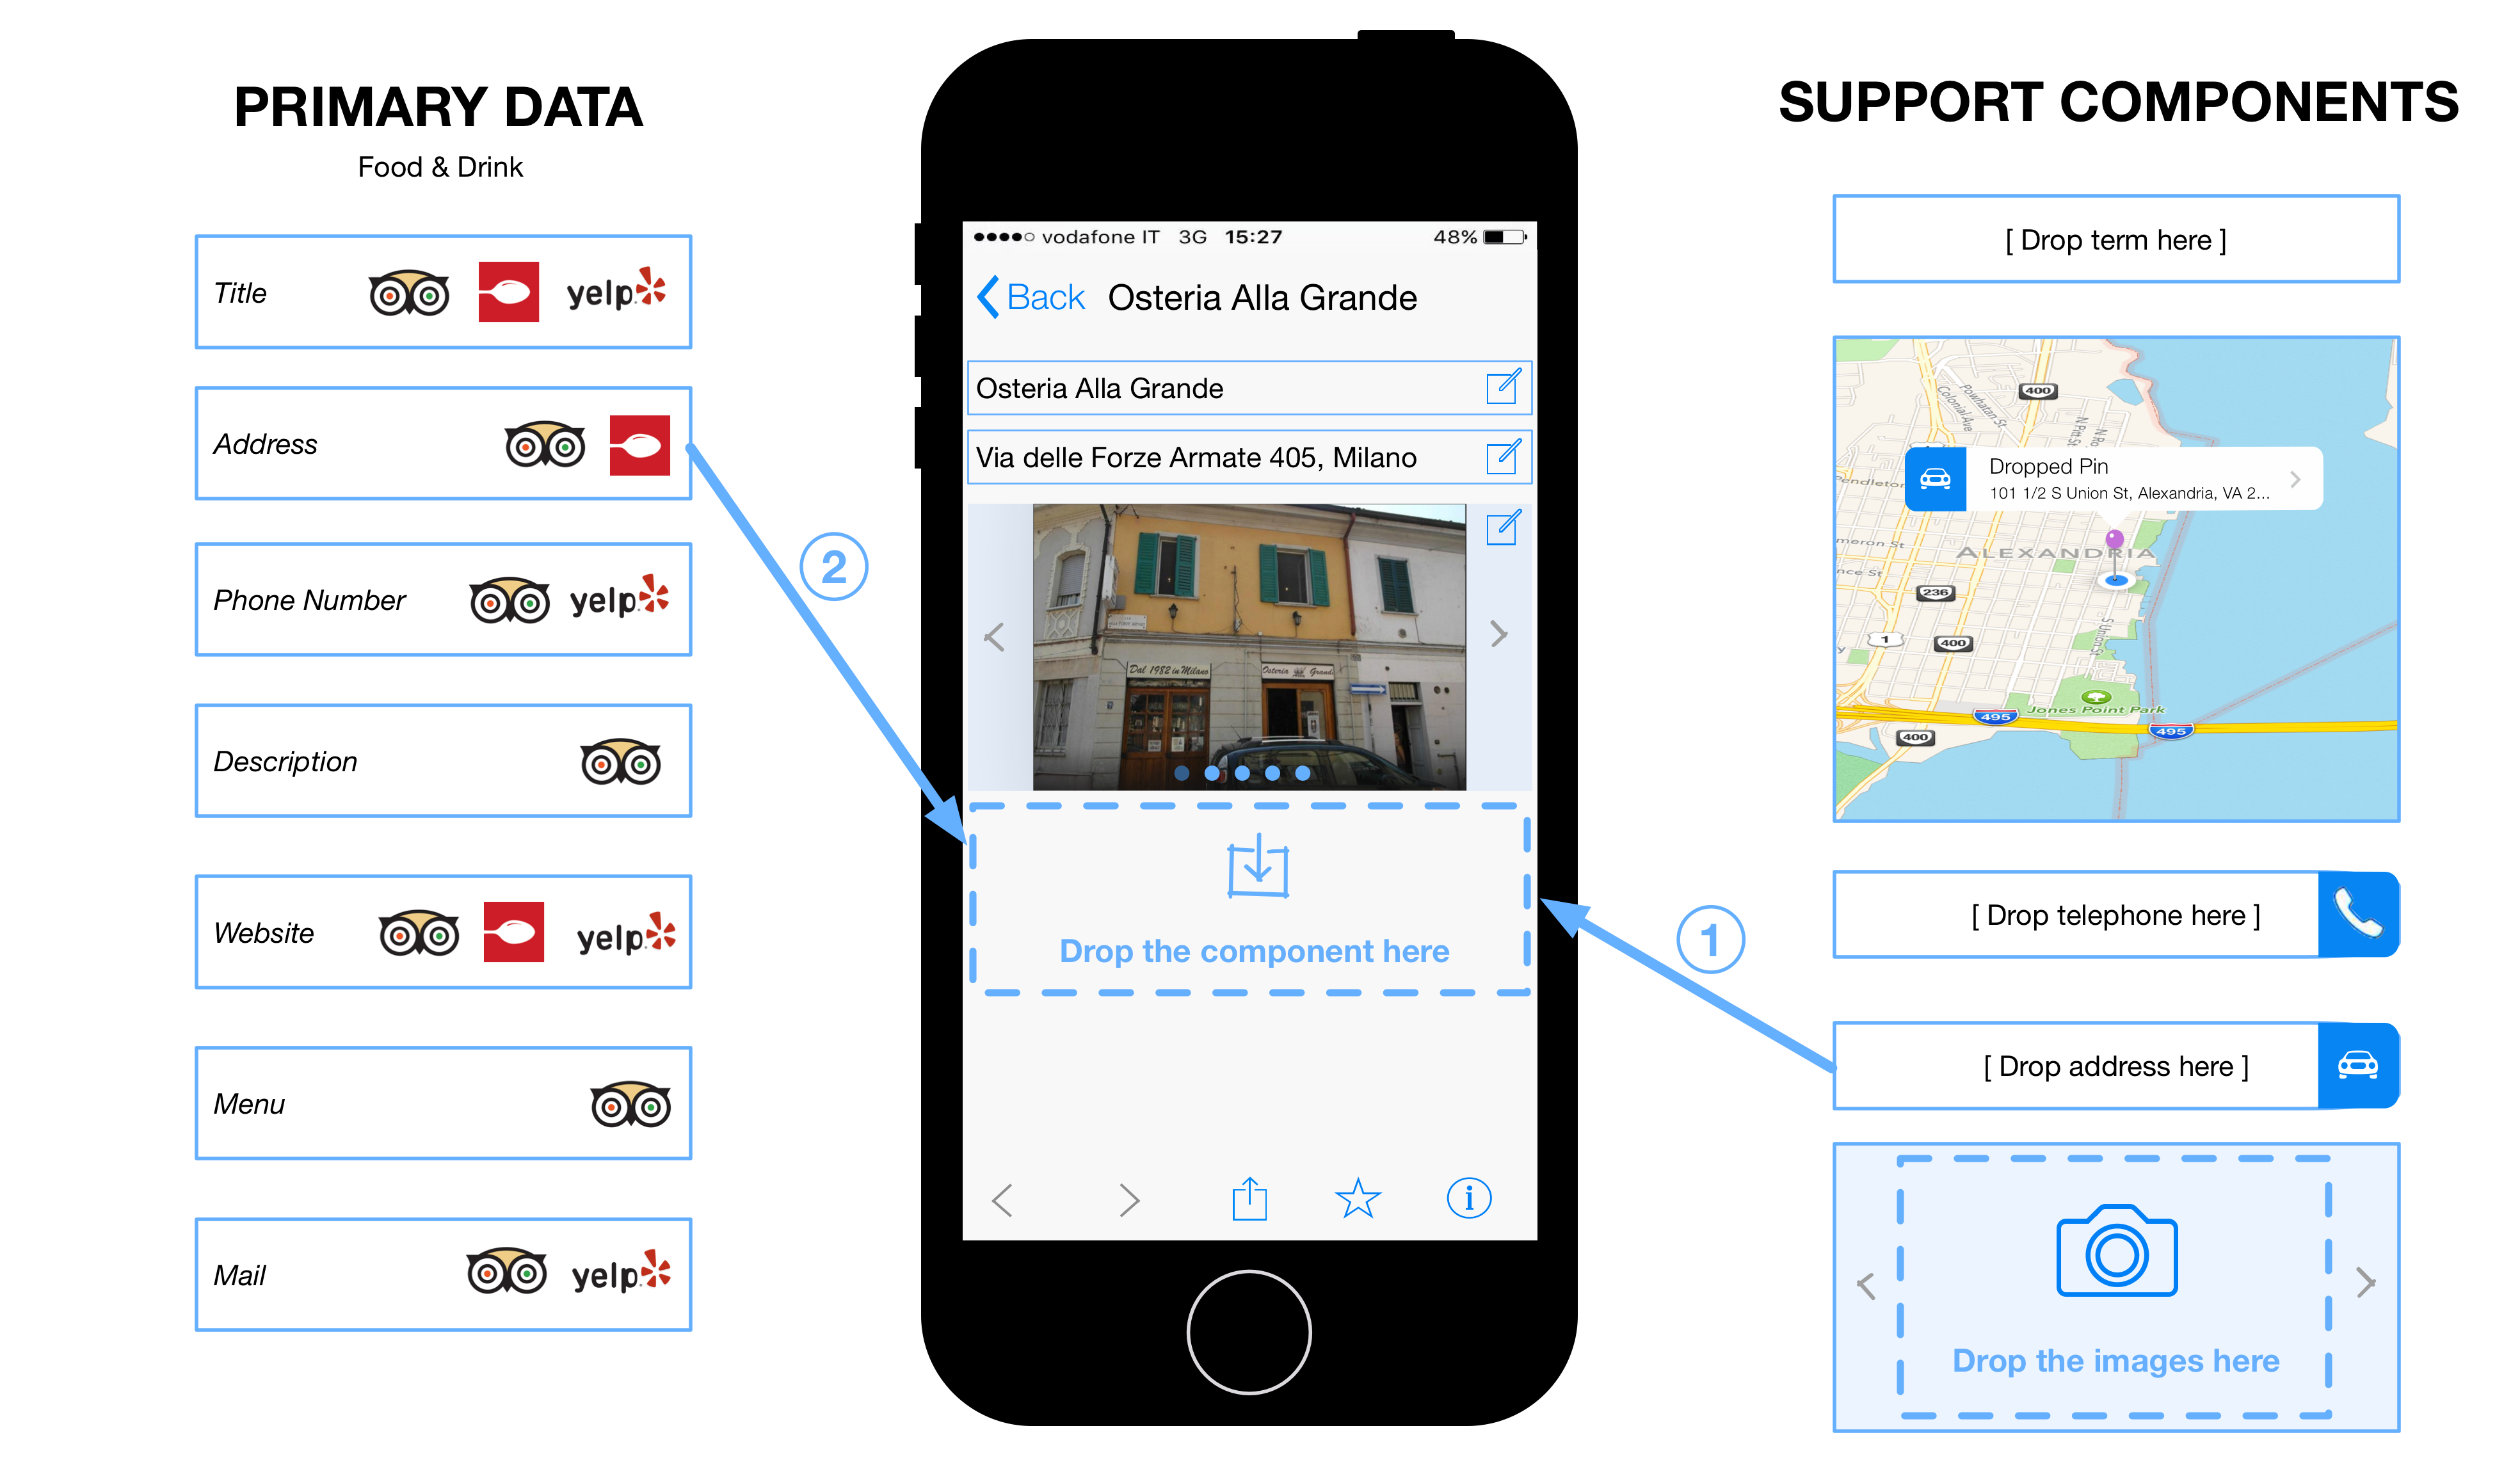
\includegraphics[width=\textwidth]{4-metodologia/Immagini/visual-mapping-nuovo.png}
	\caption{Web App di Visual Mapping}\label{fig:visual-mapping}
\end{figure}

Un altro aspetto fondamentale del sistema � legato all'utilizzo dei mashup per costruire le view dell'applicazione mobile e per associare a ogni singolo elemento il termine da richiedere al server. Questo compito viene svolto dall'\emph{esperto di settore} per mezzo della web app di Visual Mapping (Figura \ref{fig:visual-mapping}), la quale genera uno schema che definisce come e quali informazioni vengono mostrate all'utente.

\upe stato scelto di adottare due tipologie di schemi fondamentali, uno per la lista dei risultati e uno per i dettagli dell'elemento selezionato, perch� fondamentalmente sono queste due le pagine dell'applicazione che necessitano di associazioni dei termini con gli elementi grafici.
Gli schemi generati possono essere ulteriormente differenziati per due motivi principali:

\begin{enumerate}
	\item Il primo di essi � la tipologia dei dati, che nel nostro caso viene differenziata usando il parametro dell'\emph{Interest Topic}.
	Ad esempio se viene selezionato \virgolette{Food and Drink} pu� essere necessario visualizzare dati diversi rispetto a \virgolette{Museum}. Anche se ci sono parametri in comune, come \emph{Titolo}, \emph{Indirizzo}, \emph{Numero di telefono}, ci possono essere parametri peculiari, come il tipo di cucina per il primo caso o il tipo di museo per il secondo caso. Questi dati possono essere visualizzati quindi in maniera differente, e si � scelto di utilizzare oltre ad una differenziazione a livello di termini, anche di lasciare libert� di scelta per quanto riguarda il design del mashup. 
	\item
	Il secondo aspetto � la possibilit� di differenziare i dati da mostrare a livello di utente, dato che non a tutti gli utenti possono interessare le stesse informazioni oppure pu� essere preferibile mostrare i dati e le view in maniera differente in stili grafici e componenti. Infatti, una volta generato lo schema, viene associato allo specifico utente, in maniera tale da essere disponibile su richiesta della mobile app, dopo che � stato effettuato l'accesso.
	Nella web app l'esperto seleziona l'utente al quale deve generare l'applicazione e, in aggiunta alle modifiche al CDT evidenziate nella Sezione \ref{sec:cdt-su-misura}, carica gli schemi predefiniti che verranno utilizzati come base per lo schema personalizzato per l'utente. In questo modo ogni utente dell'applicazione pu� avere i propri mashup personalizzati.
	In aggiunta alla definizione dei termini nei mashup, � possibile aggiungere le propriet� stilistiche relative al singolo schema, se diverse da quelle definite globalmente.
\end{enumerate}

\begin{figure}[ht]
	\centering
	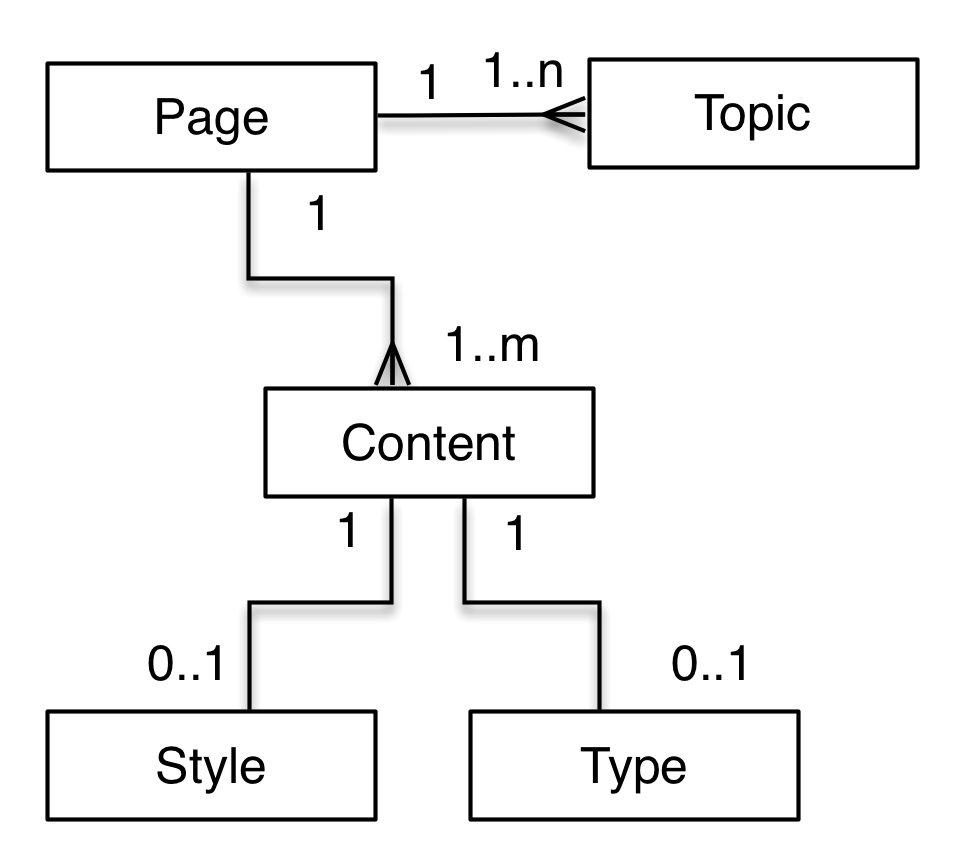
\includegraphics{4-metodologia/Immagini/view-schema.png}
	\caption{Schema delle views}\label{fig:view-schema}
\end{figure}
Lo schema delle view che � stato adottato � raffigurato nella Figura \ref{fig:view-schema}. Ad ogni pagina definita viene associato uno o pi� valori di \virgolette{Interest Topic}, perch� pu� essere che uno schema venga utilizzato per pi� di un ambito. Ogni pagina pu� avere pi� di un contenuto al quale � associato opzionalmente uno stile e la tipologia del contenuto, che servir� all'app per renderizzare il componente associato.

Per personalizzare uno schema, al \emph{designer} spettano i seguenti passaggi:

\begin{itemize}
	\item \textbf{Associazione dei termini} 
	L'associazione dei termini viene effettuata mediante \emph{drag} \& \emph{drop} dove i singoli termini sono collegati allo specifico componente della view. 
	I termini possono essere acquisiti da una repository mantenuta sul server o da una \emph{knowledge base}\footnote{\url{http://schema.org/}}, che permette di associare un significato semantico ad ogni termine in modo da agevolare l'interoperabilit� dei dati, e il designer pu� scegliere se utilizzarli tutti o solo una parte nella creazione dello schema, in modo che a runtime l'applicazione possa richiedere solamente i dati necessari alla popolazione della view.
	Nella Figura \ref{fig:visual-mapping} viene mostrata la sequenza di operazioni che deve compiere il designer e che vengono elencati di seguito:
	\begin{enumerate}
		\item Selezione del componente da inserire nella schermata del telefono e modifica dello stile a seconda delle opzioni disponibili
		\item Associazione del termine tra l'elenco di tutti quelli disponibili
	\end{enumerate}
	Ad esempio, per mostrare il titolo dell'elemento selezionato l'esperto deve selezionare un campo di testo dai componenti, trascinarlo all'interno del dispositivo virtuale e associare il campo titolo dai termini sulla sinistra della web app. A questo punto � possibile modificare alcuni elementi di stile che, definiti sullo schema, sovrascrivono eventuali stili presenti nello schema predefinito.
	%allungare questa parte
	\item \textbf{Associazione dei servizi di supporto}
	Come spiegato nella Sezione \ref{sec:ecosistema-servizi}, i servizi di supporto hanno la funzione di arricchire le informazioni che sono fornite dai servizi primari. La loro integrazione nei mashup pu� essere fatta principalmente in due modi:
	\begin{enumerate}
	\item La prima possibilit� � di associare ad un termine una app gi� installata sul device. Si consideri il caso d'uso del turismo e un servizio di ristoranti che restituisce un numero di telefono: questo dato pu� essere collegato al dialer di default per effettuare direttamente una chiamata o all'app di gestione degli SMS. Oppure l'indirizzo email pu� essere associato alla funzione \virgolette{Crea Email} dell'app predefinita di gestione della posta elettronica. Un altro esempio pu� essere quello di associare il browser di sistema al sito ufficiale o alle pagine Facebook del ristorante
	\item La seconda possibilit� riguarda invece l'utilizzo di un modulo che mostri direttamente i risultati dei servizi di supporto all'interno dell'app. 
	Questa possibilit� pu� essere utilizzata per mostrare nuovi dati relativi a un singolo elemento proveniente dai servizi primari, ad esempio le informazioni sulla posizione. In questo modo � possibile associare una mappa oppure una segnalazione che indica la distanza o i tempi di percorrenza, oppure, citando sempre l'esempio dei locali, i mezzi pubblici, car sharing o taxi che si possono utilizzare per raggiungere il ristorante
	\end{enumerate}
	
\end{itemize}

\section{Architettura utilizzata\label{sec:architettura-sistema}}

I fattori discriminanti nella scelta dell'architettura pi� idonea riguardano quale componente del sistema avr� il compito di interrogare i servizi per acquisire le informazioni da mostrare all'utente e l'integrazione dei dati.
Per quanto riguarda l'interrogazione dei servizi sono state valutate due possibilit� diametralmente opposte:

\begin{itemize}
	\item \textbf{Client centric} In questa tipologia tutte le richieste verso i servizi esterni vengono eseguite sul dispositivo, che si occuper� inoltre di integrare le informazioni ricevute e contattare i servizi di supporto
	\item \textbf{Server centric} In questa tipologia di architettura tutto il carico computazionale viene gestito dal server. Quando viene effettuata una richiesta, sar� quindi il server ad occuparsi di contattare i servizi necessari a recuperare i dati, integrare le informazioni ricevute e contattare i servizi di supporto definiti nello schema di mashup per arricchire il precedente dataset
\end{itemize}

Nel caso \emph{Mobile centric} il vantaggio � dato principalmente dal fatto che ogni dispositivo esegue le query e le operazioni che occorrono e, data la non indifferente potenza di calcolo dei moderni processori montati negli smartphone di ultima generazione, la complessit� computazionale non introduce problemi.
Purtroppo in questo modo non � possibile fare caching tra diversi utenti. Per esempio, se due utenti eseguono la medesima ricerca di ristoranti a Milano in zona Duomo verso Google Places o TripAdvisor, partiranno due query uguali per ogni servizio e, aumentando il numero di utenti, la quantit� di richieste aumenta considerevolmente, portando alla saturazione le API key con un numero limitato di richieste (es.: le API di Google). Inoltre il fatto di eseguire query verso i servizi esterni comporta un aumento del consumo energetico del device, non solo per la quantit� di dati che le interfacce di rete devono gestire, ma anche per la necessit� di eseguire le operazioni sui dati di \emph{Merge} e \emph{Union}, definite nella sezione \ref{sec:mobile-mashup}. 
Esiste anche un problema legato alla sincronizzazione dei descrittori dei servizi: nel caso in cui ne vengano aggiunti di nuovi o modificati alcuni gi� esistenti, si rende necessario un aggiornamento su tutte le applicazioni che utilizzano i descrittori coinvolti dalle modifiche.

Il caso \emph{Server centric} permette di ottenere dei miglioramenti ai problemi sopra citati. In particolare � possibile fare \emph{caching} dei risultati a livello multiutente, cio� se arrivano due query uguali con un breve intervallo l'una dall'altra, il server effettuer� una singola richiesta verso il servizio esterno e i dati della seconda richiesta verranno recuperati dalla cache. In particolare, il caching permette di ridurre il problema del numero limitato di richieste che possono essere effettuate tramite una particolare API key. Un altro aspetto che viene risolto � il fatto di non avere praticamente limiti computazionali ed energetici, perch� un server pu� elaborare pi� velocemente e in maniera pi� efficiente i dati. Il dispositivo mobile non ha pi� il carico computazionale del caso \emph{Client centric}, ma sfrutta la potenza di calcolo del server, che permette di ricevere i dati gi� elaborati con \emph{Merge} e \emph{Union}. Anche i descrittori dei servizi non hanno pi� il problema di essere distribuiti in ogni singolo device in seguito ad un aggiornamento: una volta che uno di essi viene modificato sul server, � gi� pronto e funzionante per tutte le richieste verso quel servizio.
Uno degli svantaggi principali di questa architettura � di avere un unico collo di bottiglia per tutto il sistema, che sarebbe ovviamente il server. Si dovr� dimensionare correttamente le capacit� computazionali del sistema per permettere l'evasione rapida delle richieste anche in situazioni di elevato carico, cio� quando diversi utenti effettuano nello stesso istante un vasto numero di richieste. Inoltre si presenta un problema che riguarda l'interrogazione dei servizi di supporto: questo compito dovrebbe essere ripetuto dal server per ogni elemento appartenente alla risposta che deve essere inviata al client. Molte richieste potrebbero essere invece evitate, in quanto le informazioni messe a disposizione dai servizi di supporto hanno validit� nella pagina di dettaglio di ogni elemento: non � detto che l'utente selezioni tutti gli elementi di un risposta ma generalmente ne visualizza una porzione ristretta \textcolor{red}{necessario qualche paper?}. Nel lavoro precedente \cite{rizzo2015progettazione} si era scelto di utilizzare un'architettura di tipo ibrido, dove per� il carico di complessit� era collocato principalmente nell'applicazione mobile.

\begin{figure}[h]
	\centering
	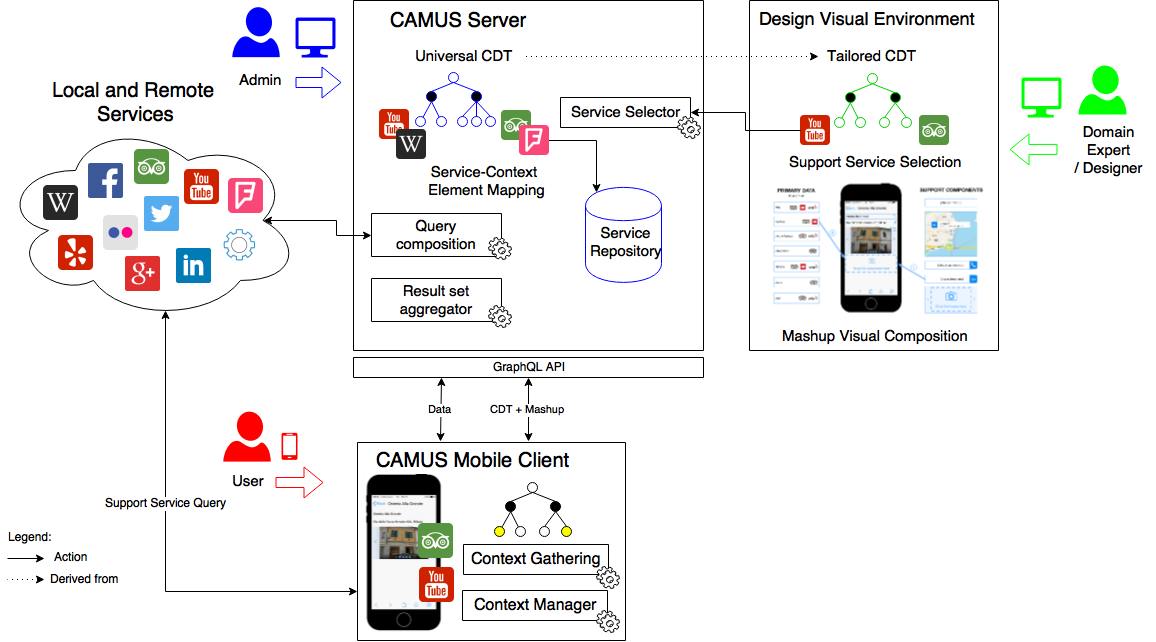
\includegraphics[width=\textwidth]{4-metodologia/Immagini/architettura-generale.png}
	\caption{Architettura del sistema}\label{fig:architettura-sistema}
\end{figure}

Come evidenziato nella Figura \ref{fig:architettura-sistema}, si � scelto di utilizzare sempre un sistema di tipo ibrido, ma spostando l'elaborazione del contesto, l'esecuzione delle richieste verso i servizi esterni e l'integrazione dei dati lato server. All'applicazione mobile vengono invece delegati i compiti di rendering dell'interfaccia grafica tramite gli schemi di mashup e l'interrogazione dei servizi di supporto per acquisire le informazioni utili ad arricchire i dati forniti dal server. Questa tecnica ha il vantaggio di ottimizzare il numero di richieste che vengono effettuate verso i servizi di supporto, limitandone il numero a quelle strettamente necessarie, che corrispondo al numero di elementi che l'utente decide di visualizzare nel dettaglio.

 Di seguito vengono elencati i tre componenti principali del sistema CAMUS:

\begin{enumerate}
	\item \textbf{Server} Il server � il punto in cui si interfaccia l'\emph{amministratore} di sistema ed � il punto dal quale � possibile avere una visione della complessit� del sistema senza astrazioni. L'\emph{amministratore} ha i compiti di registrare i nuovi servizi e di configurare i termini per la trasformazione dei risultati ricevuti dai servizi. Inoltre definisce l'albero di contesto globale, che verr� utilizzato come base per la creazione di quelli personalizzati per gli utenti e di associare le operazioni ai vari nodi che compongono l'albero
	
	\item \textbf{Web App} Le web app sono collegate all'\emph{esperto di settore} che compone l'applicazione mobile. Questo attore non � necessariamente un esperto di informatica e della tecnologia utilizzata, quindi ha bisogno di un astrazione maggiore rispetto all'amministratore. Sono disponibili due funzionalit� di base: una permette di creare dei CDT personalizzati per gli utenti e di modificare le associazioni dei servizi, mentre l'altra permette di creare i mashup per le pagine dell'applicazione, collegando i termini con i componenti che verranno poi renderizzati in fase di esecuzione
	
	\item \textbf{App Mobile} La mobile app � l'interfaccia dell'\emph{utente} finale con il sistema. Essa ha il compito di renderizzare i mashup definiti dall'esperto e di permettere all'utente di specificare il proprio contesto per richiedere al server i risultati inerenti ad esso. Oltre alle informazioni richieste all'utente vengono inoltre sfruttati i sensori messi a disposizione dal dispositivo (es.: coordinate geografiche, orario, ecc.) per migliorare la precisione del contesto, in modo trasparente all'utente.
	Una volta che l'utente finale ha effettuato l'accesso, vengono caricati gli schemi di mashup e l'albero di contesto specifico dell'utente. L'app si occuper� di renderizzare gli schemi ricevuti generando dinamicamente delle schermate che verranno utilizzate dall'utente per effettuare tutte le operazioni che desidera.
	I risultati vengono mostrati seguendo il pattern \emph{master-detail} \cite{molina2002user}: in prima istanza viene generato un elenco (\emph{master}) dei risultati ottenuti, mostrando poche informazioni riguardo il singolo elemento; successivamente l'utente pu� selezionare uno o pi� elementi della lista per visualizzare i dettagli (\emph{detail}) dell'elemento. In questa fase entrano in gioco i servizi di supporto: una volta che l'utente decide di visualizzare i dettagli di un elemento, l'app si occupa, in base allo schema di mashup corrente, di interrogare i servizi di supporto necessari per arricchire le informazioni che ha precedentemente ricevuto.
\end{enumerate}

\textcolor{red}{Aggiungere sequence diagram di una richiesta in generale?}



\chapter{Progettazione di dettaglio e implementazione del backend\label{ch:implementazione-backend}}

In questo capitolo ...

\section{Architettura e tecnologie utilizzate\label{sec:architettura-backend}}

In questa sezione verranno analizzate le tecnologie utilizzate per sviluppare il backend di CAMUS e, in seguito, l'architettura adottata.

La logica del sistema � sviluppata a partire da Node.js\footnote{Node.js: \url{https://nodejs.org/en/}}, un framework per lo sviluppo di applicazioni web basato sul linguaggio Javascript\footnote{Javascript Documentation: \url{https://developer.mozilla.org/en/docs/Web/JavaScript}}. Alla base viene utilizzato il motore Javascript V8 di Google. Node.js permette la creazione di web server tramite l'ausilio di diversi \emph{moduli} che gestiscono le funzionalit� di base, come il file system, le operazioni di rete, la crittografia, ecc. \upe compatibile con i sistemi operativi pi� diffusi e possono essere utilizzati tutti i linguaggi che riescono ad essere compilati in Javascript, come CoffeScript o TypeScript. Per certi versi, Node.js pu� essere considerato molto simile a PHP come ambito di utilizzo, la principale differenza � che le funzioni in Node.js non sono bloccanti, quindi � possibile eseguire attivit� in parallelo e utilizzare callback o promise per segnalare il completamento, sia in caso positivo che negativo, dei comandi. Questa scelta di utilizzare un'architettura di tipo \emph{event-driver} permette la realizzazione di web server estremamente scalabili senza coinvolgere l'utilizzo dei thread. Node.js infatti lavora solo su un singolo core, tranne ne caso in cui vengano avviate pi� istanze separate in parallelo, ed il parallelismo gestito tramite eventi permette di simulare un sistema multithread, riducendo per� in maniera significativa la complessit� di sviluppo.

Come database � stato scelto di utilizzare MongoDB\footnote{MongoDB: \url{https://www.mongodb.org/}}. MongoDB � un database che fa parte della categoria NoSQL, in quanto abbandona lo schema relazionale classico basato su tabelle in favore di uno basato sui documenti. Ogni documento ha una struttura simile ad un file JSON, in MongoDB in particolare viene nominato BSON, e possiede uno schema dinamico, a differenza dei database relazioni che hanno uno schema ben definito. Questa caratteristica permette di sviluppare in maniera pi� semplice e rapida le applicazioni e di integrare facilmente alcune tipologie di dato. La struttura a documento prevede per� una ristrutturazione generale dello schema di un database. Per esempio, per chi � abituato ad un database relazione, deve essere consapevole che in MongoDB non esiste l'operatore di JOIN, bens� viene fornita la possibilit� di salvare dei sotto-documenti all'interno di un documento. Per esempio, se si vuole memorizzare un libro che ha pi� autori, � possibile salvare l'elenco degli autori, insieme ad eventuali altri suoi dati, all'interno del documento contenente le informazioni del libro\footnote{Questo � solo un esempio indicativo, non � una soluzione ottima in quanto un autore pu� pubblicare pi� di un libro e utilizzando questo schema si otterrebbe una duplicazione delle informazioni}. Un'altra caratteristica di MongoDB � la flessibilit� nel comporre le query, che possono essere specificate sui campi, su un range di valori o tramite un'espressione regolare. Sono sempre ammesse anche proiezioni dei campi che si vogliono visualizzare nei risultati. Sempre per interrogare i dati si possono utilizzare funzioni \emph{MapReduce} e di \emph{aggregazione}. In particolare quest'ultimo permette di ottenere un risultato simile all'operatore GROUP BY dei database SQL, ma fornisce anche la flessibilit� di concatenare pi� operazioni per formare una \emph{pipeline}. Mette a disposizione anche il comando \$lookup per effettuare una unione tra documenti diversi. MongoDB permette di definire degli \emph{indici} sui campi che vengono utilizzati di frequente nelle query per velocizzarle. Una caratteristica che rende MongoDB estremamente scalabile � la possibilit� di eseguire multiple istanze su macchine diverse, permettendo al sistema di scalare orizzontalmente. Sar� compito di MongoDB gestire le chiamate e selezionare il nodo dove effettuare la richiesta, tramite un sistema di load-balancing. Tutto questo viene agevolato dalla struttura del file system utilizzato da MongoDB, chiamato \emph{Grid File System}, che gestisce la divisione dei documenti in diversi \virgolette{pezzi}. Oltre al load-balancing per migliorare le prestazioni � possibile anche utilizzare altre macchine come \emph{repliche}, in modo da garantire la sicurezza dei dati nel caso di guasti.

Il fatto che MongoDB memorizzi i file in un formato dalla struttura molto simile ad un JSON agevola l'integrazione con Node.js, che a sua volta utilizza oggetti semplicemente mappabili in formato JSON. Come specificato precedentemente, MongoDB non possiede una struttura definiti a priori. Per garantire comunque una consistenza dei dati salvati nel database, si � scelto di forzare l'utilizzo di uno schema tramite un Object Relational Mapping (ORM)\footnote{Object Relational Mapping: \url{https://it.wikipedia.org/wiki/Object-relational_mapping}}. Un ORM fornisce un livello di astrazione superiore ad un driver nativo e permette la definizione di come gli oggetti vengono mappati nel database e viceversa, definendo quindi uno schema del database. In particolare, per il progetto CAMUS � stato utilizzato un ORM specifico per Node.js di nome mongoose\footnote{MongooseJS: \url{http://mongoosejs.com/}}.

Oltre ad un database che garantisse la persistenza dei dati pi� importanti, si � resa necessaria l'adozione di un altro database per effettuare  caching delle risposte ricevute dai servizi e per mantenere alcune informazioni relative alle sessioni degli utenti per un determinato intervallo di tempo. La scelta in questo caso � ricaduta su Redis\footnote{Redis: \url{http://redis.io/}}. Redis fornisce un database interamente memorizzato in memoria, quindi estremamente rapido nell'evadere le richieste, ed � basato su un sistema chiave-valore. Queste caratteristiche, insieme al fatto che quanto viene salvato un dato � possibile impostare un intervallo di tempo scaduto il quale l'elemento viene eliminato, lo ha reso il candidato perfetto per svolgere questo compito. Per interfacciare Node.js con l'istanza di Redis in esecuzione viene utilizzato il modulo ioredis\footnote{ioredis: \url{https://github.com/luin/ioredis}}.

\begin{figure}[ht]
	\centering
	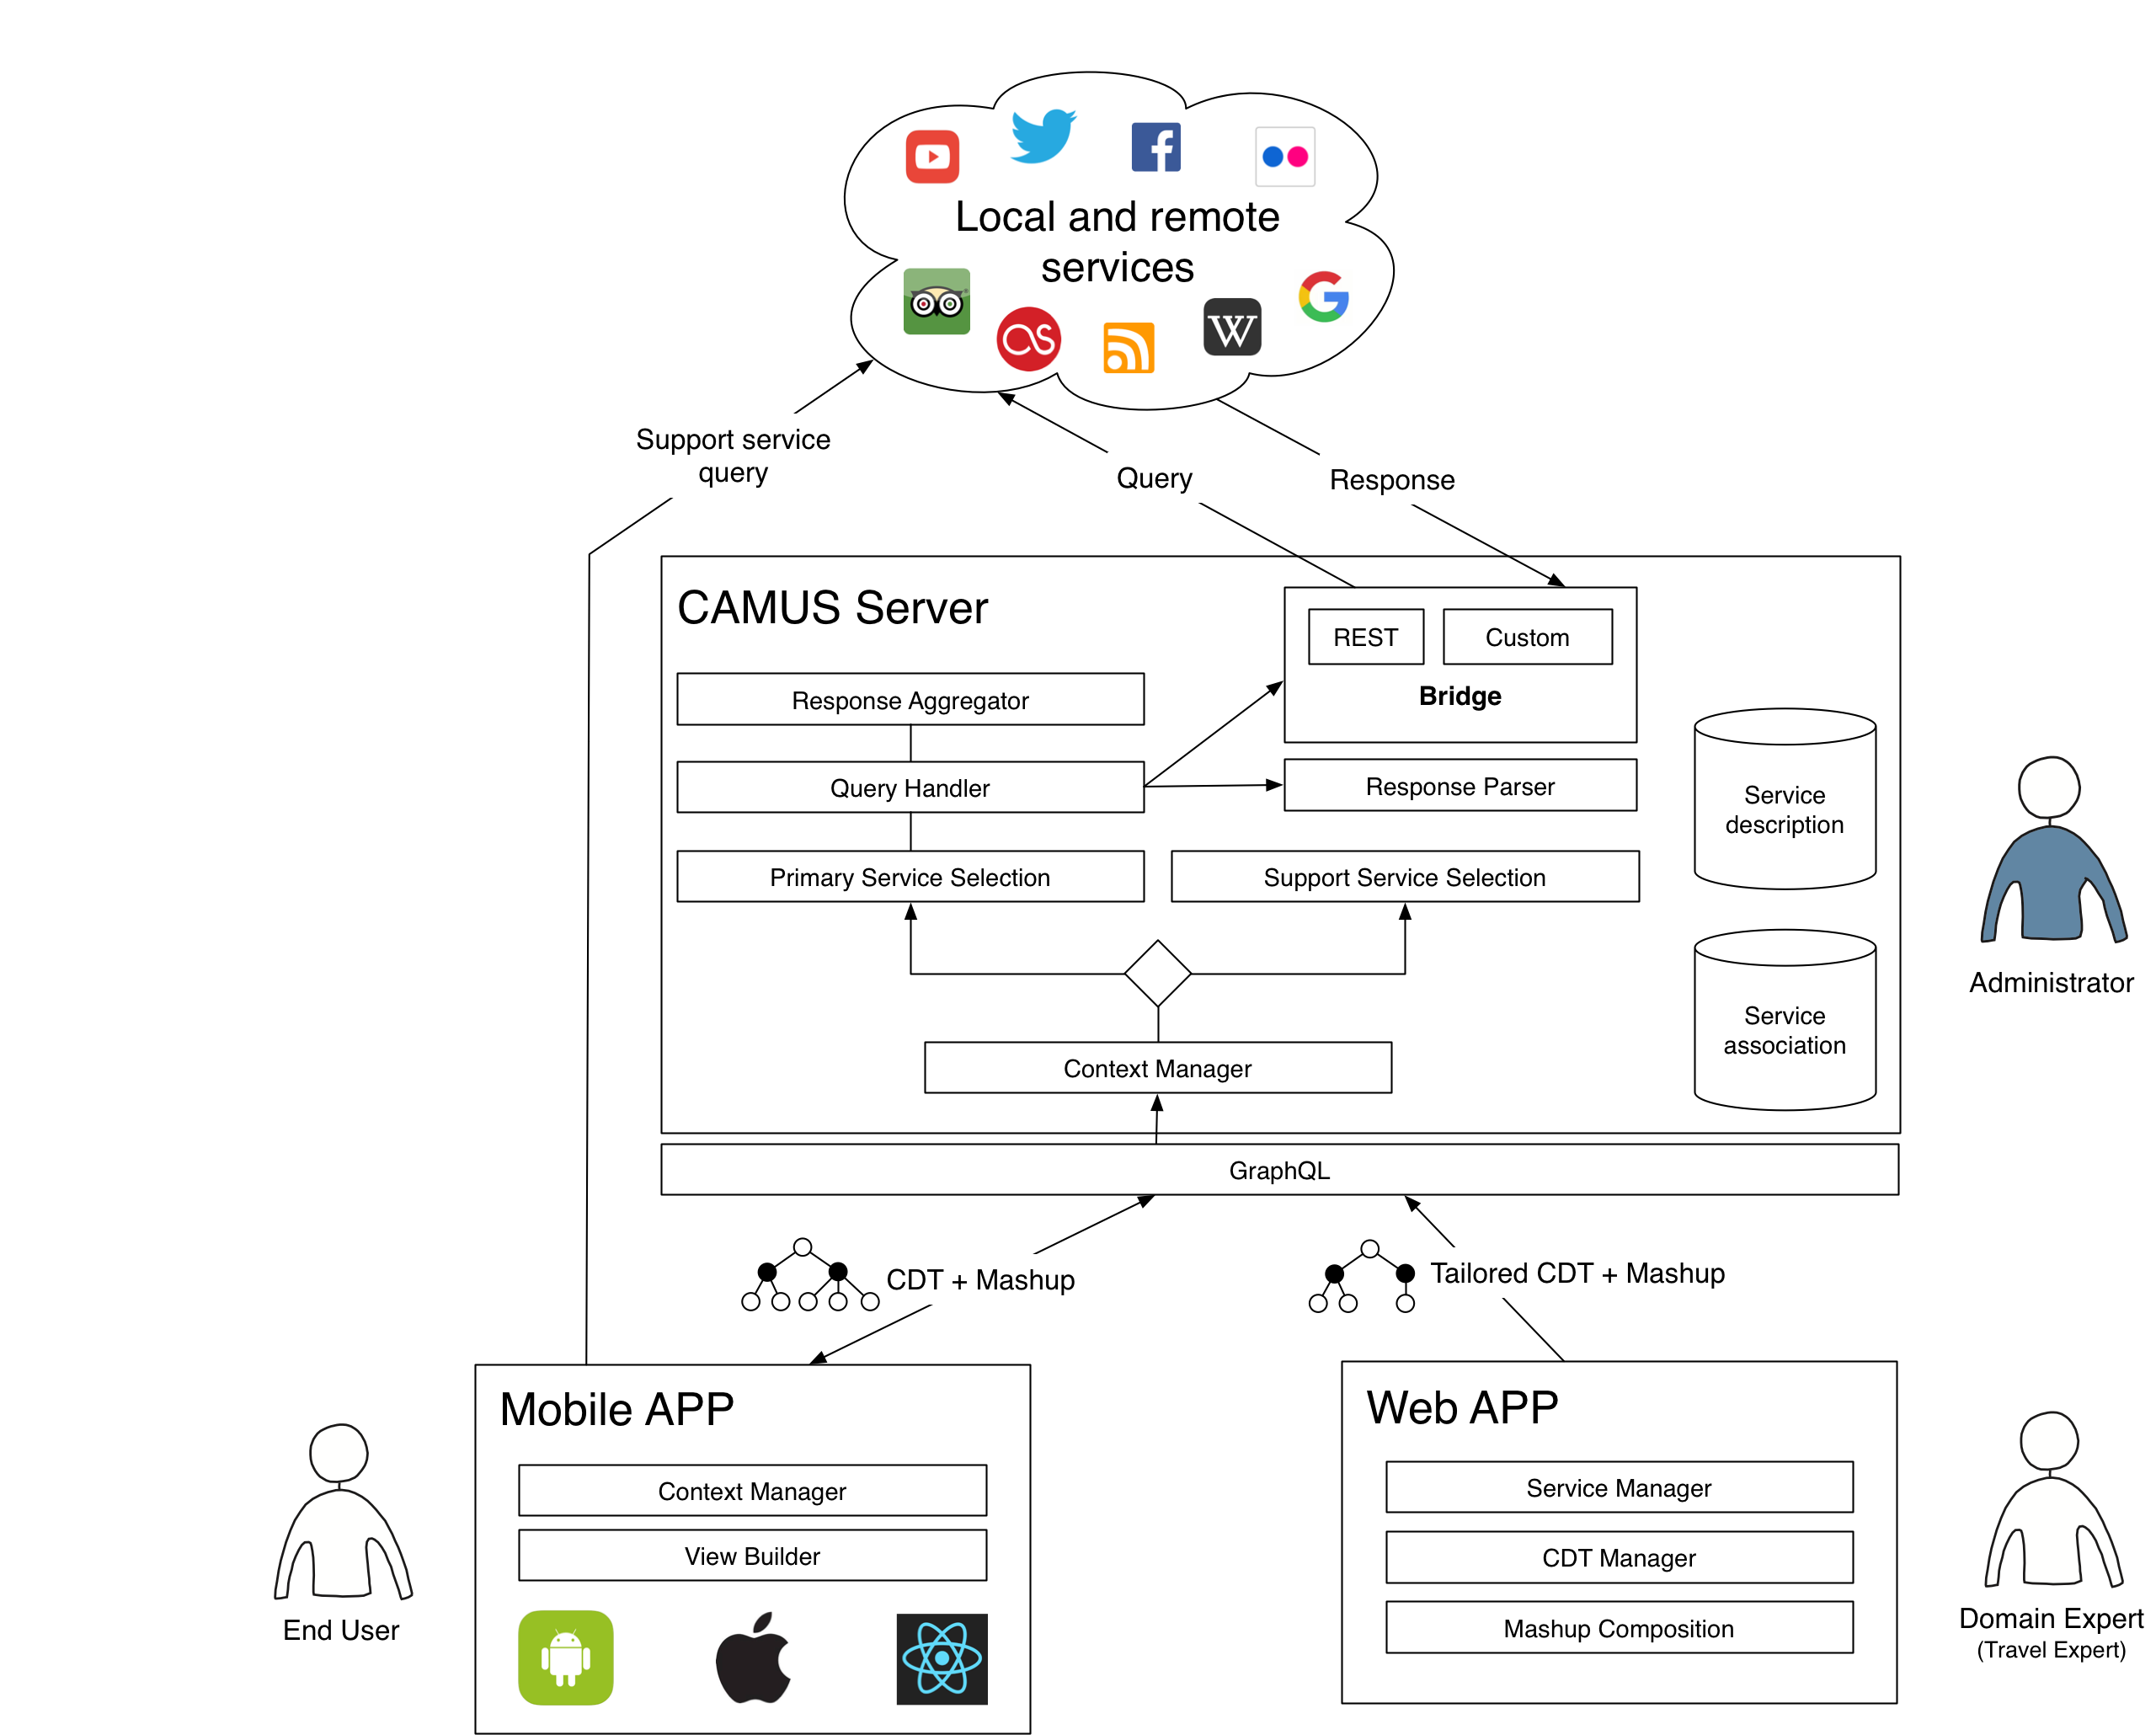
\includegraphics[width=\textwidth]{5-implementazione-backend/Immagini/camus-architecture.png}
	\caption{Architettura del backend}\label{fig:architettura-backend}
\end{figure}

Ora che sono state definite le tecnologie utilizzate, viene presentata l'architettura di CAMUS, che pu� essere osservata nello schema in Figura \ref{fig:architettura-backend}. Come si pu� notare � stata privilegiata la modularit� dei vari componenti che formano il sistema, in modo che ognuno sia circoscritto ad uno specifico compito. Inoltre, tutti i componenti mostrati sono \emph{stateless}, cio� non mantengono informazioni sullo stato di una sessione. Questa scelta architetturale permette di poter avviare diverse istanze del backend di CAMUS in modo che le richieste degli utenti possano essere evase da un'istanza piuttosto che un'altra.

Il componente che sta alla base di tutti gli altri � l'\emph{Execution Helper}. Il suo compito � quello di inizializzare tutti gli altri componenti ed organizzare le chiamate secondo il flusso della richiesta, che verr� analizzato nel dettaglio nella Sezione \ref{sec:flusso-richiesta-server}.

Il \emph{Context Manager} � il componente che si occupa di ricevere il contesto inviato dalla mobile app e lo trasforma in una versione \virgolette{decorata}, eseguendo una unione tra le informazioni ricevute dal client e quelle del descrittore completo del CDT. In questo modo viene agevolata l'esecuzione dei componenti successivi, in quanto le informazioni necessarie all'elaborazione sono gi� state catalogate e definite in modo corretto.

Il compito del \emph{Primary Service Selection} � di andare a recuperare le associazioni tra l'albero di contesto e le operazioni dei servizi primari. \upe inoltre suo compito gestire le associazioni personalizzate, come quella relativa la ricerca tramite \emph{localit�}. In seguito assegna un \emph{punteggio} ad ogni operazione trovata ed emette le prime N operazioni con valutazione pi� elevata.

Un compito simile viene svolto dal \emph{Support Service Selection} per le operazioni di supporto. Sebbene lo scopo del componente sia lo stesso, l'algoritmo di selezione � differente: in questo caso le associazioni vengono considerate pi� come \emph{vincoli}, ed un'operazione, per essere selezionata, deve rispettare tutti i vincoli associati.

Il \emph{Query Handler} ha il compito di gestire le chiamate verso i servizi. Prende in input la lista di operazioni scelte dal \emph{Primary Service Selection} e ne acquisice i \emph{descrittori}, contenenti le informazioni per poterli interrogare. Di seguito organizza le chiamate ai servizi attraverso l'uso di \emph{bridge} specifici, che sono scelti in base al \emph{protocollo} di comunicazione adottato dal servizio. Una volta ricevute le risposte, si occupa di interfacciarsi con il \emph{Response Parser} per trasformarle nella rappresentazione interna tramite l'utilizzo dei \emph{termini semantici} come nome dei campi.

Infine, il \emph{Response Aggregator} ha il compito di analizzare gli elementi ricevuti al fine di rimuovere i duplicati.

In questa sezione si � voluta dare una visione d'insieme sui compiti che spettano ai vari componenti. Un'analisi pi� approfondita delle attivit� di ognuno di essi verr� svolta nella Sezione \ref{sec:componenti-backend}.

\section{Descrittore dell'albero di contesto\label{sec:descrittore-albero-contesto}}

Nella Sezione \ref{sec:context-dimension-model} � stato esposto il modello del \emph{Context Dimension Tree}. In questa sezione viene invece definito come l'albero di contesto viene descritto nel sistema. Sono state effettuate alcune semplificazioni per agevolare la memorizzazione ed il recupero delle informazioni. Nelle seguenti sottosezioni vengono analizzati nel dettaglio i singoli oggetti che formano un albero di contesto.

\subsection{Radice}

Questo oggetto rappresenta la radice di un albero di contesto. \upe composto dai seguenti parametri:

\begin{itemize}
	\item \textbf{User Id} L'elenco degli utenti a quali questo albero � indirizzato. Viene lasciata la possibilit� di definire pi� utenti perch� uno stesso albero pu� essere valido per pi� utenti con un profilo simile
	\item \textbf{Context} Contiene i \emph{nodi} che compongono l'albero. Per una descrizione approfondita si fa riferimento alla Sezione \ref{sec:nodo-cdt}
	\item \textbf{Default Values} Vengono elencati tutti i valori che l'\emph{esperto di settore} ha deciso siano sempre validi per gli utenti ai quali questo albero viene associato. \upe composto dal nome della \emph{dimensione} e dal relativo \emph{valore} che assume
\end{itemize}

Viene inoltre definito un \emph{CDT Globale}, che viene utilizzato come base per la creazione di quelli specifici per ogni utente. Questo albero ha la particolarit� che non viene associato a nessun utente.

\subsection{Nodo\label{sec:nodo-cdt}}

Questo oggetto rappresenta un nodo dell'albero. In particolare vengono rappresentati solamente i nodi di tipo \emph{dimensione}, mentre per i nodi \emph{contesto} e \emph{parametro} vengono rappresentati in altri oggetti. Ogni nodo possiede i seguenti attributi:

\begin{itemize}
	\item \textbf{Name} Rappresenta il nome del nodo dimensione
	\item \textbf{For} Descrive la tipologia di nodo, che verr� utilizzata per assegnare un peso utile nella fase di \emph{selezione delle operazioni} e per attribuire un valore ai parametri nella fase di \emph{invocazione dei servizi}. I valori ammessi sono \emph{filter}, \emph{parameter} o \emph{ranking}. Vengono inoltre ammesse le combinazioni \emph{filter}|\emph{parameter} e \emph{ranking}|\emph{parameter}: un nodo pu� essere solamente di tipo \emph{filter} o \emph{ranking}, al fine dell'assegnamento dei pesi, mentre pu� essere anche di tipo \emph{parameter}, in quanto indica che verr� utilizzato anche nella fase di composizione delle query. Se viene definito il tipo \emph{parameter} devono essere assegnati diversi \emph{parametri}, per specificarne le caratteristiche
	\item \textbf{Values} Elenca i possibili valori che pu� assumere il nodo. Questo elenco corrisponde ai nodi di tipo \emph{contesto} del modello del CDT
	\item \textbf{Parameters} L'elenco dei parametri associati al nodo. Per ulteriori dettagli su questo oggetto si fa riferimento alla Sezione \ref{sec:parametro-cdt}
	\item \textbf{Parents} Contiene l'elenco di tutti i nodi dimensione dai quali discende il nodo corrente. Viene utilizzato per effettuare l'unione delle sottodimensioni di un nodo
\end{itemize}

Esempio di nodo:

\begin{lstlisting}[backgroundcolor = \color{lightgray}]
	{
		"name": "InterestTopic",
		"for": "filter",
		"values": [
			"Restaurant",
			"Cinema",
			"Theater",
			"Hotel",
			"Museum",
			"Event"
		]
	}
\end{lstlisting}

\subsection{Parametro\label{sec:parametro-cdt}}

Definisce i parametri che sono associati ad un nodo dimensione. Corrisponde ai nodi di tipo \emph{parametro} del modello del CDT. \upe composto dai seguenti campi:

\begin{itemize}
	\item \textbf{Name} Definisce il nome del parametro. Corrisponde al nome che viene definito dall'operazione per identificare il parametro. Questo campo verr� utilizzato in fase di composizione della query per invocare il servizio ed � quindi essenziale che equivalga al nome fornito dal gestore del servizio
	\item \textbf{Type} Il/I formato/i del dato che vengono accettati
	\item \textbf{Enum} Questo campo viene utilizzato quando non si vuole lasciare all'utente la possibilit� di specificare valori a suo piacimento ma � necessario che scelga tra alcune opzioni obbligatorie
	\item \textbf{Fields} Questo elenco permette di definire dei campi che vanno ulteriormente a specificare il parametro. Un esempio viene dato dal parametro \virgolette{Localit�}, che pu� essere specializzato nei campi \virgolette{Latitudine} e \virgolette{Longitudine}
\end{itemize}

Esempio di parametro:

\begin{lstlisting}[backgroundcolor = \color{lightgray}]
	{
		"name": "Location",
		"for": "ranking|parameter",
		"parameters": [
			{
				"name": "CityCoord",
				"fields": [
					{
						"name": "Latitude"
					},
					{
						"name": "Longitude"
					}
				]
			}
		]
	}
\end{lstlisting}

\section{Descrittore dei servizi\label{sec:descrittore-servizi}}

In CAMUS l'acquisizione dei dati avviene tramite servizi, come descritto nella Sezione \ref{sec:utilizzo-servizi}. Affinch� il sistema possa effettuare le richieste, � necessario che sia presente una formato per descrivere le caratteristiche di ogni servizio (es.: l'indirizzo verso il quale effettuare la richiesta, i parametri da inserire, ecc.). Per questo motivo � stato introdotto l'utilizzo di un \emph{descrittore dei servizi}, che sia in grado di descrivere tutte le possibili configurazioni che i servizi possono richiedere. I \emph{descrittori} non sono altro che file JSON che specificano le impostazioni di ogni servizio. Di seguito verranno analizzati nel dettaglio tutti i campi che compongono il descrittore. Visto che il descrittore contiene una moltitudine di informazioni che riguardano diversi aspetti di un servizio, viene diviso in sotto-oggetti in modo da semplificarne la comprensione e lettura.

\subsection{Oggetto principale}

\upe il punto di partenza per la descrizione di un servizio. Comprende i seguenti campi:

\begin{itemize}
	\item \textbf{Name} \upe il nome associato al servizio
	\item \textbf{Description} Fornisce una descrizione delle funzionalit� del servizio
	\item \textbf{Protocol} Definisce la tipologia con la quale accedere al servizio. Pu� assumere i valori \virgolette{rest}, \virgolette{query} o \virgolette{custom}, per specificare rispettivamente che il servizio viene invocato secondo la logica rest, viene composta una query con parametri o necessita di un metodo particolare per l'accesso
	\item \textbf{Base Path} Rappresenta l'indirizzo di base del servizio. A partire da questo indirizzo verr� composto quello completo aggiungendo in coda i percorsi specifici delle \emph{operazioni} richieste. Non deve essere aggiunta al termine nessuna slash (\virgolette{/})
	\item \textbf{Operazioni} L'elenco delle operazioni esposte dal servizio. Per un approfondimento riguardo questo oggetto fare riferimento alla Sezione \ref{sec:descrittore-operazioni}
\end{itemize}

Esempio di oggetto principale:

\begin{lstlisting}[backgroundcolor = \color{lightgray}]
  {
	  "name": "GooglePlaces",
	  "protocol": "query",
	  "basePath": "https://maps.googleapis.com/maps/api/place",
	  "operations": [ ... ]
  }
\end{lstlisting}

\subsection{Operazioni\label{sec:descrittore-operazioni}}

Rappresenta le operazioni che sono messe a disposizione dal servizio. Un'operazione viene descritta come di seguito:

\begin{itemize}
	\item \textbf{Name} Il nome dell'operazione
	\item \textbf{Type} Rappresenta la tipologia dell'operazione. Un'operazione pu� essere \emph{primaria} o di \emph{supporto}. Questa distinzione viene utilizzata principalmente per permettere la catalogazione delle operazioni da mostrare nelle web app
	\item \textbf{Description} La descrizione dell'attivit� svolta dall'operazione
	\item \textbf{Path} Il percorso specifico per richiamare l'operazione. Questo valore viene aggiunto al \emph{Base Path} del servizio. Deve essere sempre preceduto da una slash (\virgolette{/})
	\item \textbf{Bridge Name} Questo campo � opzionale, definisce il nome del bridge con la logica necessaria per invocare il servizio. \upe obbligatorio quando per il servizio viene utilizzato il protocollo \emph{custom}
	\item \textbf{Parameters} Definisce l'elenco dei parametri accettati in input dall'operazione. Per ulteriori dettagli su questo oggetto si fa riferimento alla Sezione \ref{sec:descrittore-parametri}
	\item \textbf{Headers} In questo oggetto vengono definiti gli attributi da aggiungere all'header della richiesta. Questo oggetto viene definito nella Sezione \ref{sec:descrittore-header}
	\item \textbf{Response Mapping} Serve per definire le regole di associazione per mappare la risposta del servizio coi termini semantici utilizzati dal sistema. Maggiori dettagli sui campi di questo oggetto vengono discussi nella Sezione \ref{sec:descrittore-risposta}
	\item \textbf{Pagination} Serve a raccogliere gli attributi necessari per gestire la paginazione specifica di ogni servizio. Sono supportati meccanismi di paginazioni basati sul \emph{numero di pagina} o su \emph{token}. Questo oggetto viene analizzato nel dettaglio nella Sezione \ref{sec:descrittore-paginazione}
\end{itemize}

Esempio di operazione:

\begin{lstlisting}[backgroundcolor = \color{lightgray}]
	{
		"name": "nearBySearch",
		"type": "primary",
		"path": "/nearbysearch/json",
		"parameters": [ ... ],
		"responseMapping": { ... },
		"pagination": { ... }
	}
\end{lstlisting}

\subsection{Parametri\label{sec:descrittore-parametri}}

In quest'oggetto vengono definiti i parametri di input di un operazione. I parametri generalmente sono composti da un campo che ne definisce il \emph{nome} e dal rispettivo valore. In alcuni casi per� vengono accettati pi� di un valore. Il descrittore deve dunque essere in grado di gestire questa situazione. Un ulteriore compito affidato a questo oggetto � quello di acquisire il valore di un determinato parametro dal \emph{contesto}. Viene inoltre fornito un semplice sistema di traduzione dei dati acquisiti dal contesto, per permettere le trasformazioni verso un valore idoneo per l'operazione corrente. Infine, soprattutto per le operazioni di \emph{supporto}, viene permessa un'associazione del parametro verso uno o pi� \emph{termini semantici}, per permettere all'app mobile di conoscere l'attributo dove andare a recuperare il valore concreto a run-time. Nello specifico, l'oggetto � cos� composto:

\begin{itemize}
	\item \textbf{Name} Il nome del parametro. Questo campo � \emph{obbligatorio}, in quanto definisce il nome che verr� utilizzato per comporre la query per richiedere i dati
	\item \textbf{Description} La descrizione della tipologia del parametro
	\item \textbf{Required} Specifica se il parametro corrente � obbligatorio o meno in una richiesta. Non definire questo attributo equivale ad assegnargli valore \emph{false}
	\item \textbf{Type} Definisce il \emph{tipo} di dato che l'operazione si aspetta di ricevere. Le principali tipologie di dato che vengono inviate verso i servizi sono \emph{stringhe}, \emph{numeri} o \emph{date}
	\item \textbf{Default} Indica un valore predefinito per il parametro. Questo campo particolarmente utile per la web app relativa il \emph{Visual Mapping}, in quanto permette di ricevere degli esempi di risposta dai servizi da mostrare all'utente
	\item \textbf{Collection Format} Questo campo definisce il \emph{separatore} da utilizzare in caso siano presenti pi� di un valore per il parametro. Sono accettati i seguenti quattro separatori: \emph{i)} csv, comma separated values; \emph{ii)} ssv, space separated values; \emph{iii)} tsv, tab separated values; \emph{iv)} pipes. Se non specificato viene utilizzato di default il tipo \emph{csv}
	\item \textbf{Mapping CDT} Definisce uno o pi� nodi dell'albero di contesto dove andare ad acquisire il valore ricevuto dalla mobile app. Nel caso vengano associati pi� di un nodo, viene seguito l'ordine di definizione nella fase di composizione della query
	\item \textbf{Mapping Term} Definisce uno o pi� termini semantici da associare al parametro. Questi termini vengono utilizzati a run-time per andare ad acquisire il valore del parametro dalle risposte ricevute dai servizi primari
	\item \textbf{Translate} Questo oggetto viene utilizzato quando � necessario effettuare un modifica del/i valore/i acquisiti dall'albero di contesto. \upe formato dai campi \virgolette{from} e \virgolette{to}, che specificano rispettivamente il valore di \emph{origine} e quello \emph{tradotto}. Vengono definite tante traduzioni quanti sono i valori che pu� assumere il rispettivo nodo del CDT
\end{itemize}

Esempio di parametro:

\begin{lstlisting}[backgroundcolor = \color{lightgray}]
	{
		"name": "Location",
		"required": true,
		"default": "-33.8670522,151.1957362",
		"collectionFormat": "csv",
		"mappingCdt": [
			"CityCoord.Latitude",
			"CityCoord.Longitude"
		]
	}
\end{lstlisting}

\subsection{Header\label{sec:descrittore-header}}

Quest'oggetto definisce i campi che compongono l'header associato ad una richiesta. \upe composto dai seguenti campi:

\begin{itemize}
	\item \textbf{Name} Rappresenta il nome del campo da specificare nell'header
	\item \textbf{Value} Definisce il valore che assume il campo
\end{itemize}

\subsection{Formato della risposta\label{sec:descrittore-risposta}}

In quest'oggetto sono definite le regole con le quali vengono trasformate le risposte ricevute dal servizio nel formato interno a CAMUS, dove ogni attributo viene associato ad un rispetto \emph{termine semantico} che ne definisce il contenuto. In particolare, vengono utilizzati i seguenti campi:

\begin{itemize}
	\item \textbf{List} Definisce il l'attributo che contiene l'elenco dei risultati. \upe utile nei casi in cui la risposta, oltre ai risultati, contiene al suo interno anche dei metadati relativi l'interrogazione. Se non specificato si assume che l'elenco dei risultati incominci dalla root della risposta
	\item \textbf{Items} Vengono mappati i vari campi che compongono ogni oggetto dei risultati. In particolare vengono definiti il \virgolette{percorso} dal quale recuperare il valore ed il \virgolette{termine semantico} da associare. I campi che non vengono mappati saranno ignorati dal processo di trasformazione e le relative informazioni andranno perdute. \upe necessario dunque effettuare l'operazione di mapping delle risposte con attenzione, in modo da garantire la gestione di risposte complete
	\item \textbf{Functions} Viene permesso l'utilizzo di funzioni specifiche per trasformare i valori. Questa funzione riceve in ingresso il parametro \virgolette{value}, che rappresenta il valore corrente del campo, e deve restituire il nuovo valore che verr� sostituito a quello originale. Oltre alla funzione specifica, � necessario definire anche l'\emph{attributo} sul quale eseguire questa trasformazione. L'attributo equivale al \emph{termine semantico} definito nel punto precedente
\end{itemize}

Esempio di formato di risposta:

\begin{lstlisting}[backgroundcolor = \color{lightgray}]
	{
		"list": "results",
		"items": [
			{
				"termName": "title2,
				"path": "name"
			},
			{
				"termName": "address",
				"path": "vicinity"
			},
			{
				"termName": "latitude",
				"path": "geometry.location.lat"
			},
			{
				"termName": "longitude",
				"path": "geometry.location.lng"
			}
		],
		"functions": [
			{
				"onAttribute": "latitude",
				"run": "return String(value)"
			},
			{
				"onAttribute": "longitude",
				"run": "return String(value)"
			}
		]
	}
\end{lstlisting}

\subsection{Paginazione\label{sec:descrittore-paginazione}}

In quest'oggetto vengono gli attributi necessari per gestire la paginazione delle risposte. In particolare il sistema � in grado di gestire due tecniche di paginazione, quella basata sul \emph{numero di pagina} e quella che utilizza dei \emph{token} per richiamare le pagine. L'oggetto � composto dai seguenti campi:

\begin{itemize}
	\item \textbf{Attribute Name} Specifica il nome del parametro da aggiungere alla query per richiamare una specifica pagina
	\item \textbf{Type} Definisce il meccanismo di paginazione da utilizzare. Sono ammessi due valori: \virgolette{number} per la paginazione basata sul numero di pagine e \virgolette{token}, per quella che sfrutta i token per richiamare le pagine successive
	\item \textbf{Token Attribute} Serve per definire dove andare a leggere nella risposta il token relativo alla pagina successiva
	\item \textbf{Page Count Attribute} Definisce l'attributo che fornisce l'informazione del numero di pagine totale che possono essere richieste
\end{itemize}

Esempio di paginazione:

\begin{lstlisting}[backgroundcolor = \color{lightgray}]
	{
		"pagination": {
			"attributeName": "pagetoken",
			"type": "token",
			"tokenAttribute": "next_page_token"
		}
	}
\end{lstlisting}

\section{Schema del database}

La base di dati viene utilizzata principalmente per garantire la persistenza di tre elementi: \emph{i)} il descrittore dei servizi, \emph{ii)} l'albero del contesto e \emph{iii)} le associazioni tra operazioni e nodi del CDT.

Queste entit� permettono al sistema di svolgere le attivit� principali. In Figura \ref{fig:schema-er-db} viene mostrato il modello \emph{Entit�-Relazione} che sta alla base di CAMUS.

\begin{figure}[ht]
	\centering
	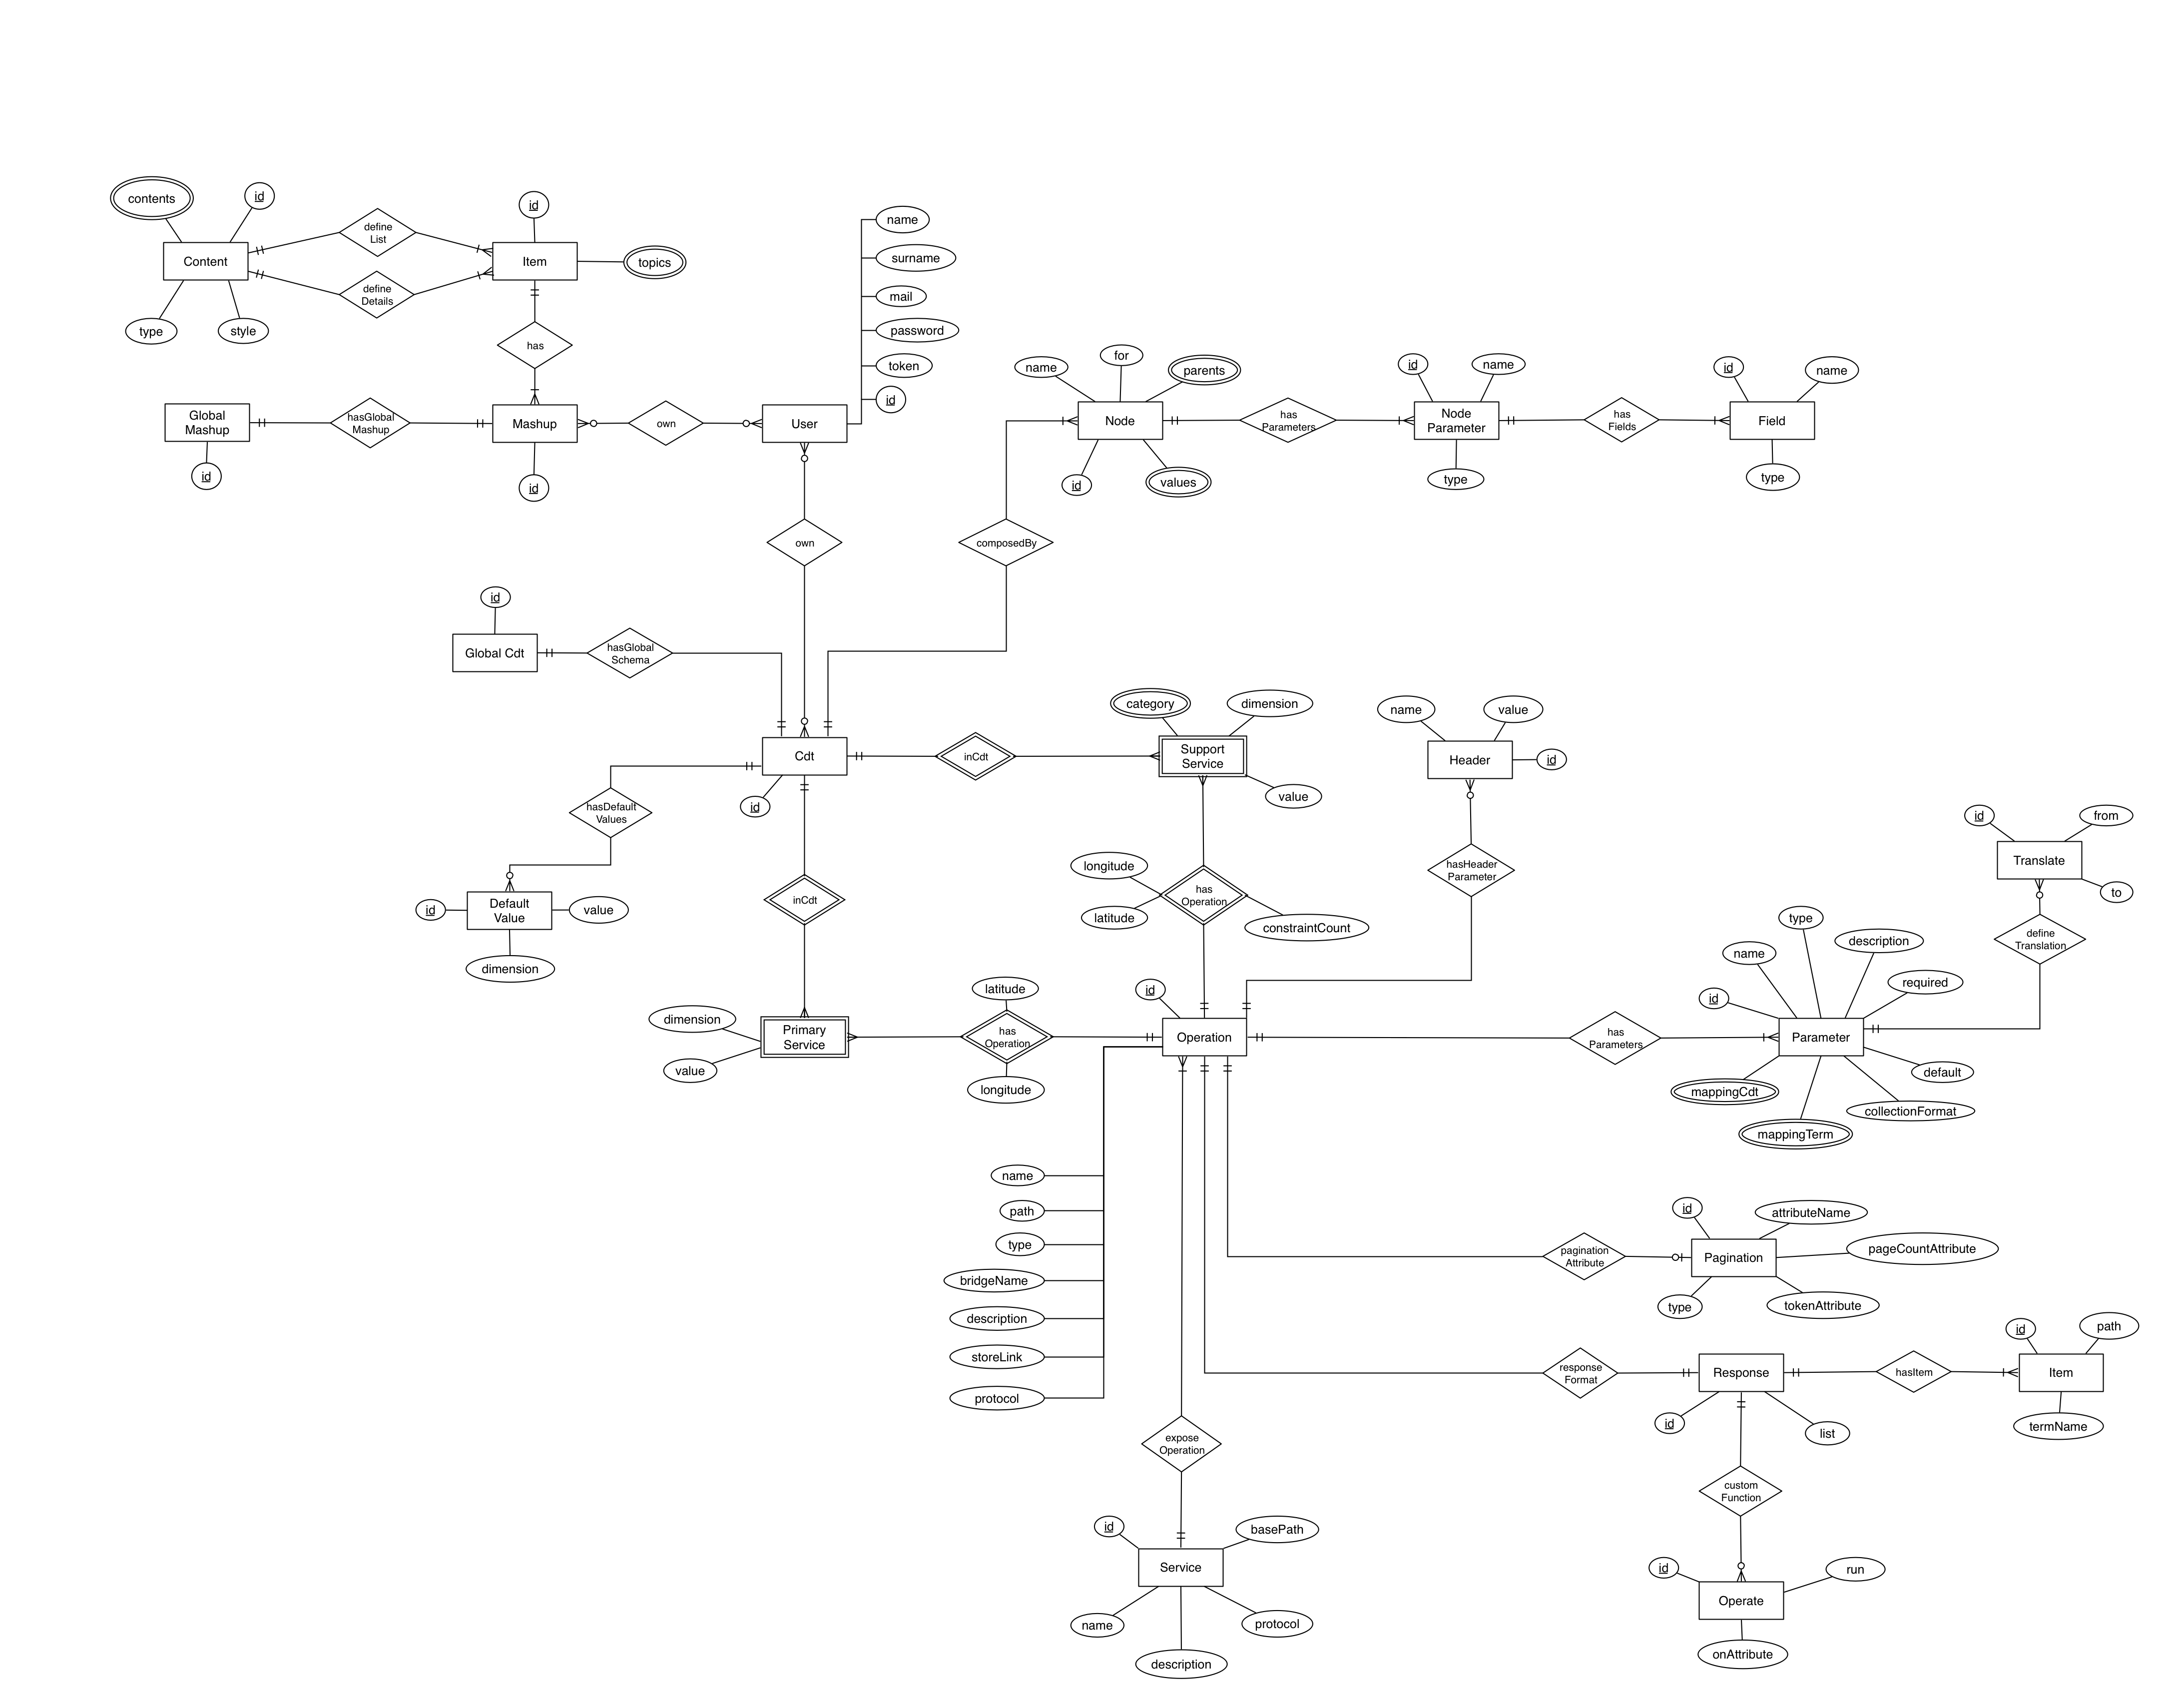
\includegraphics[width=\textwidth]{5-implementazione-backend/Immagini/schema_er_db.png}
	\caption{Diagramma ER del database}\label{fig:schema-er-db}
\end{figure}

Di seguito viene presentata una descrizione dettagliata delle entit� che compongono il modello:

\begin{itemize}
	\item \textbf{User} \upe l'entit� che rappresenta un utente. Ogni utente viene descritto dal nome, cognome, indirizzo email, password e da un token che viene utilizzato per identificare la sessione. Un utente pu� possedere nessuno o pi� CDT
	\item \textbf{Cdt} Rappresenta la radice di un albero di contesto. Un albero di contesto pu� essere posseduto da zero o pi� utenti. Il \emph{CDT Globale} � l'unico caso nel quale non vengono associati utenti, perch� � universale e quindi valido per chiunque. In tutti gli altri casi si tratta di \emph{CDT su misura}, che devono quindi essere associati ad almeno un utente. Viene lasciata la possibilit� di associazione con pi� utenti nel caso il loro profilo sia molto simile
	\item \textbf{Node} Rappresenta un nodo \emph{dimensione} del CDT e viene descritto dai seguenti attributi:
	\begin{itemize}
		\item \emph{Name} Il nome del nodo
		\item \emph{For} Descrive la tipologia del nodo, che verr� utilizzata per assegnare un peso utile nella fase di \emph{selezione delle operazioni} e per attribuire un valore ai parametri nella fase di \emph{invocazione dei servizi}. I valori ammessi sono \emph{filter}, \emph{parameter}, \emph{ranking}, \emph{filter}|\emph{parameter} o \emph{ranking}|\emph{parameter}. Se viene definito il tipo \emph{parameter} possono essere assegnati al nodo diverse entit� di tipo \virgolette{Node Parameter}, per specificarne le caratteristiche
		\item \emph{Parents} Contiene l'elenco di tutti i nodi dai quali discende il nodo corrente
		\item \emph{Values} Elenca i valori ammessi dal nodo dimensione corrente. Corrispondono ai nodi di tipo \emph{contesto} nel modello del CDT
	\end{itemize}
	\item \textbf{Node Parameter} Questa entit� rappresenta un parametro associato ad un nodo del CDT. Viene caratterizzato dai seguenti campi:
	\begin{itemize}
		\item \emph{Name} Definisce il nome del parametro
		\item \emph{Type} Il/I formato/i del dato che vengono accettati
		\item \emph{Enum} Elenca i possibili valori che pu� assumere il parametro
	\end{itemize}
	Ad un parametro possono essere associati diversi \virgolette{campi}, nel caso in cui un parametro sia definito da diversi sottoattributi. Per esempio, il parametro \emph{Localit�} pu� essere specializzato nei campi \emph{Latitudine} e \emph{Longitudine}
	\item \textbf{Field} \upe l'entit� che rappresenta un campo di un parametro. \upe composto dal \virgolette{nome} che assume ed il \virgolette{tipo}, che descrive il formato del campo
	\item \textbf{Default Value} Questa entit� elenca le coppie dimensione-valore che sono preimpostate, in quanto non subiscono variazioni per l'utente ed � inutile che gli vengano continuamente riproposte. Vengono salvati solamente il nome della \virgolette{dimensione} e il relativo \virgolette{valore}
	\item \textbf{GlobalCdt} Viene utilizzata per memorizzare l'identificato del \emph{CDT Globale}, che viene utilizzato come base per la costruzione di tutti gli alberi di contesto del sistema
	\item \textbf{Service} Entit� che rappresenta un servizio, che viene definito dai seguenti campi:
	\begin{itemize}
		\item \emph{Name} Il nome del servizio
		\item \emph{Description} Una descrizione delle operazioni che vengono svolte dal servizio
		\item \emph{Base Path} Definisce l'indirizzo base al quale � possibile contattare il servizio. Viene utilizzato insieme ai \emph{path} specifici di ogni operazione per formare l'indirizzo completo
		\item \emph{Protocol} Specifica la tipologia di servizio, che pu� assumere i valori \emph{rest}, \emph{query} o \emph{custom}. Per i primi due casi esiste un'implementazione fornita assieme al sistema mentre per l'ultimo caso � necessario specificare quale bridge specifico viene utilizzato per invocare il servizio
	\end{itemize}
	Un servizio deve esporre almeno un'\emph{operazione} per poter essere utilizzato
	\item \textbf{Operation} Un'operazione rappresenta l'elemento essenziale affinch� un servizio possa essere invocato. Possiede i seguenti attributi:
	\begin{itemize}
		\item \emph{Name} Il nome dell'operazione. Questo campo viene utilizzato principalmente per avere un riferimento intuitivo delle varie operazioni che vengono esposte da ogni servizio e pu� essere scelto a proprio piacimento
		\item \emph{Description} Descrizione dell'attivit� che viene svolta dall'operazione
		\item \emph{Path} Definisce il percorso specifico verso il quale richiamare l'operazione. Questo campo viene concatenato assieme al \emph{basePath} definito dal servizio per formare l'indirizzo completo
		\item \emph{Type} Specifica se l'operazione � di tipo \emph{primario} o di \emph{supporto}. Questa distinzione � pi� di carattere categorico che funzionale, in quanto non ci sono particolari variazioni tra le due tipologie di operazione. Viene utilizzato dal tool di \emph{Visual Mapping} per elencare nello spazio pi� appropriato le varie operazioni
		\item \emph{Bridge Name} Questo campo definisce il nome dell'implementazione specifica del bridge da utilizzare per invocare il servizio. \upe necessario che sia definito solamente nel caso in cui nel servizio � stato definito come protocollo \emph{custom}
	\end{itemize}
	Ogni operazione ha una serie di informazioni di contorno che possono essere associati. Deve obbligatoriamente definire un'entit� per descrivere il formato della \emph{risposta} che riceve e pu� esporre gli attributi necessari per gestire la \emph{paginazione} dei risultati. Possono essere associati pi� campi relativi ai valori da aggiungere all'\emph{header} della chiamata quando necessari. Affinch� un'operazione sia utilizzabile, � necessario definire almeno un \emph{parametro} per assegnare i valori che il servizio utilizzer� per comporre la risposta
	\item \textbf{Parameter} Questa entit� specifica come sono formati gli attributi che compongono un parametro. In particolare viene descritta dai seguenti campi:
	\begin{itemize}
		\item \emph{Name} Il nome del parametro
		\item \emph{Type} Il formato del valore associato al parametro
		\item \emph{Description} La descrizione della semantica del parametro
		\item \emph{Required} Valore booleano che specifica se il parametro � obbligatorio o meno per l'operazione associata. Di default assume valore \emph{false}
		\item \emph{Default} Specifica un valore predefinito, che viene utilizzato in particolare nella fase di \emph{Visual Mapping} per mostrare una risposta di esempio
		\item \emph{Collection Format} Viene utilizzato solamente nel caso in cui ci siano pi� valori associati e definisce il separatore da usare per dividere i valori. I separatori riconosciuti sono \emph{csv} (comma separated values), \emph{ssv} (space separated values), \emph{tsv} (tab separated values) e \emph{pipes}.
		\item \emph{Mapping Term} Viene utilizzato per associare il parametro ad uno dei \emph{termini semantici} conosciuti dal sistema Viene utilizzato per la composizione della query per i servizi di supporto. Possono essere definiti pi� termini
		\item \emph{Mapping Cdt} Specifica da quale nodo dell'\emph{albero di contesto} � possibile recuperare il valore da associare al parametro. Possono essere aggiunti pi� nodi verso i quali andare a cercare i valori
	\end{itemize}
	In alcuni casi pu� essere anche definita una \emph{traduzione} per permettere di trasformare il valore definito dal contesto in uno pi� idoneo per il servizio
	\item \textbf{Translate} Questa entit� definisce come effettuare una traduzione da un valore, generalmente recuperato dall'albero di contesto, verso un altro che viene riconosciuto dal servizio. Viene semplicemente descritta dai campi \virgolette{from} e \virgolette{to}, che rappresentano rispettivamente il valore originale e la sua traduzione finale
	\item \textbf{Pagination} Specifica quali sono gli attributi della risposta usati per gestire la paginazione dei risultati. In particolare, sono necessarie le seguenti informazioni:
	\begin{itemize}
		\item \emph{Attribute Name} Definisce il nome del parametro utilizzato dall'operazione per richiamare la pagina successiva. Deve corrispondere al nome fornito dal gestore del servizio
		\item \emph{Type} Specifica il tipo di paginazione utilizzata dal servizio. Il sistema supporta due tipologie: \emph{i)} number, dove viene utilizzato un numero per identificare ogni pagina; \emph{ii)} token, dove vengono generati diversi token per richiamare le diverse pagine
		\item \emph{Page Count Attribute} Indica il nome del campo della risposta che contiene il numero totale di pagine che sono disponibili per la query corrente. Viene utilizzato unicamente nel caso sia stato scelto come tipo \emph{number}. Serve al sistema per sapere fino a quando � possibile incrementare il numero di pagina per recuperare nuove informazioni
		\item \emph{Token Attribute} Indica il nome del campo della risposta che contiene il token alla pagina successiva. Viene utilizzato unicamente nel caso sia stato scelto come tipo \emph{token}. Il token recuperato viene utilizzato nella query successiva per richiedere la nuova pagina con altre informazioni. A differenza del caso precedente non � possibile sapere a priori quante siano le pagine in totale. Semplicemente, quando il servizio non fornisce pi� token significa che non sono pi� disponibili ulteriori pagine
	\end{itemize}
	\item \textbf{Header} Questa entit� definisce gli attributi che devono essere aggiunti all'header di un richiesta. \upe formato dal \virgolette{nome} del campo ed il \virgolette{valore} da associargli
	\item \textbf{Response} \upe l'entit� che descrive il formato della risposta ricevuta e definisce come mappare gli attributi che la compongono con i termini semantici. Viene utilizzato il campo \virgolette{lista} per specificare il percorso all'interno della risposta dove � possibile andare a recuperare l'elenco dei risultati. Se non specificato viene presa la radice dell'oggetto ricevuto. Inoltre vengono definite diverse associazioni con l'entit� \emph{Item}, che definisce come mappare ogni singolo elemento della risposta. In aggiunta � possibile definire delle funzioni che vengono eseguite in seguito alla fase di trasformazione, per permettere la personalizzazione dei valori ricevuti
	\item \textbf{Item} Permette di definire la regola con la quale convertire un campo della risposta nel relativo termine semantico. \upe composto dal campo \virgolette{path}, che specifica il percorso del campo, e \virgolette{termName}, che definisce il termine da associargli
	\item \textbf{Operate} Questa entit� permette la creazione di funzioni personalizzate per essere eseguite sui valori ricevuti dal servizio. \upe composta dai campi \virgolette{run}, dove viene scritto il codice (JavaScript) da essere eseguite, e \virgolette{onAttribute}, che specifica il termine coinvolto nella trasformazione. Per l'esecuzione della funzione si tenga presente che viene chiamata fornendo in input il parametro \emph{value}, che corrisponde al valore corrente del campo
	\item \textbf{Primary Service} In questa entit� vengono definite le associazioni tra le operazioni primarie e il corrispondente albero di contesto. Viene rappresentata come un'entit� debole, in quanto l'identificazione � possibile dall'identificativo del CDT e dell'operazione. Non � presente invece una relazione che colleghi quest'entit� a quella dei nodi per due motivi in particolare: \emph{i)} per come � stato scelto di rappresentare un nodo non � possibile identificare univocamente una coppia dimensione-valore \emph{ii)} per ragioni di performance � stato preferito un approccio che richiedesse il coinvolgimento di meno entit� possibili. Quindi � stata effettuata una denormalizzazione a livello di modello, definendo i campi \virgolette{dimension} e \virgolette{value} che definiscono lo specifico nodo. Viene inoltre permesso di associare un'operazione a delle coordinate geografiche, tramite la relazione \emph{hasOperation}
	\item \textbf{Support Service} In questa entit� vengono definite le associazioni tra le operazioni di supporto e il corrispondente albero di contesto. Come per le operazioni primarie, viene anch'essa rappresentata come un'entit� debole, in quanto per l'identificazione vengono utilizzati l'identificativo del CDT, quello dell'operazione e la categoria del servizio. Viene seguita la stessa logica di associazione ai nodi utilizzata in precedenza per le operazioni primarie. L'unica variante riguarda l'attributo \virgolette{constraintCount} definito sulla relazione \emph{hasOperation}. Come evidenziato nella Sezione \ref{sec:associazione-servizi-cdt}, le associazioni delle operazioni di supporto vengono considerate alla stregua di vincoli, in quanto devono tutte essere rispettate affinch� un'operazione possa essere presa in considerazione. Questo attributo viene utilizzato proprio per questo scopo: permette di sapere quanti siano i vincoli definiti per l'operazione corrente e permette quindi il funzionamento dell'algoritmo di selezione
\end{itemize}

Una volta definito il modello ER � necessario passare alla realizzazione dello \emph{schema logico} del database, quello che verr� effettivamente utilizzato nell'implementazione. Non esistendo uno standard per realizzare uno schema di questo tipo per i database non relazionali � stato scelto di utilizzare un \emph{diagramma delle classi} per rappresentare i \emph{documenti} che compongono il database. Ogni classe viene intesa come un documento ed i collegamenti tra di essi rappresentano i sottodocumenti.

In Figura \ref{fig:schema-logico-db} viene mostrato lo schema logico utilizzato per CAMUS. Le linee tratteggiate indicano le referenze tra i vari documenti.

\begin{figure}[ht]
	\centering
	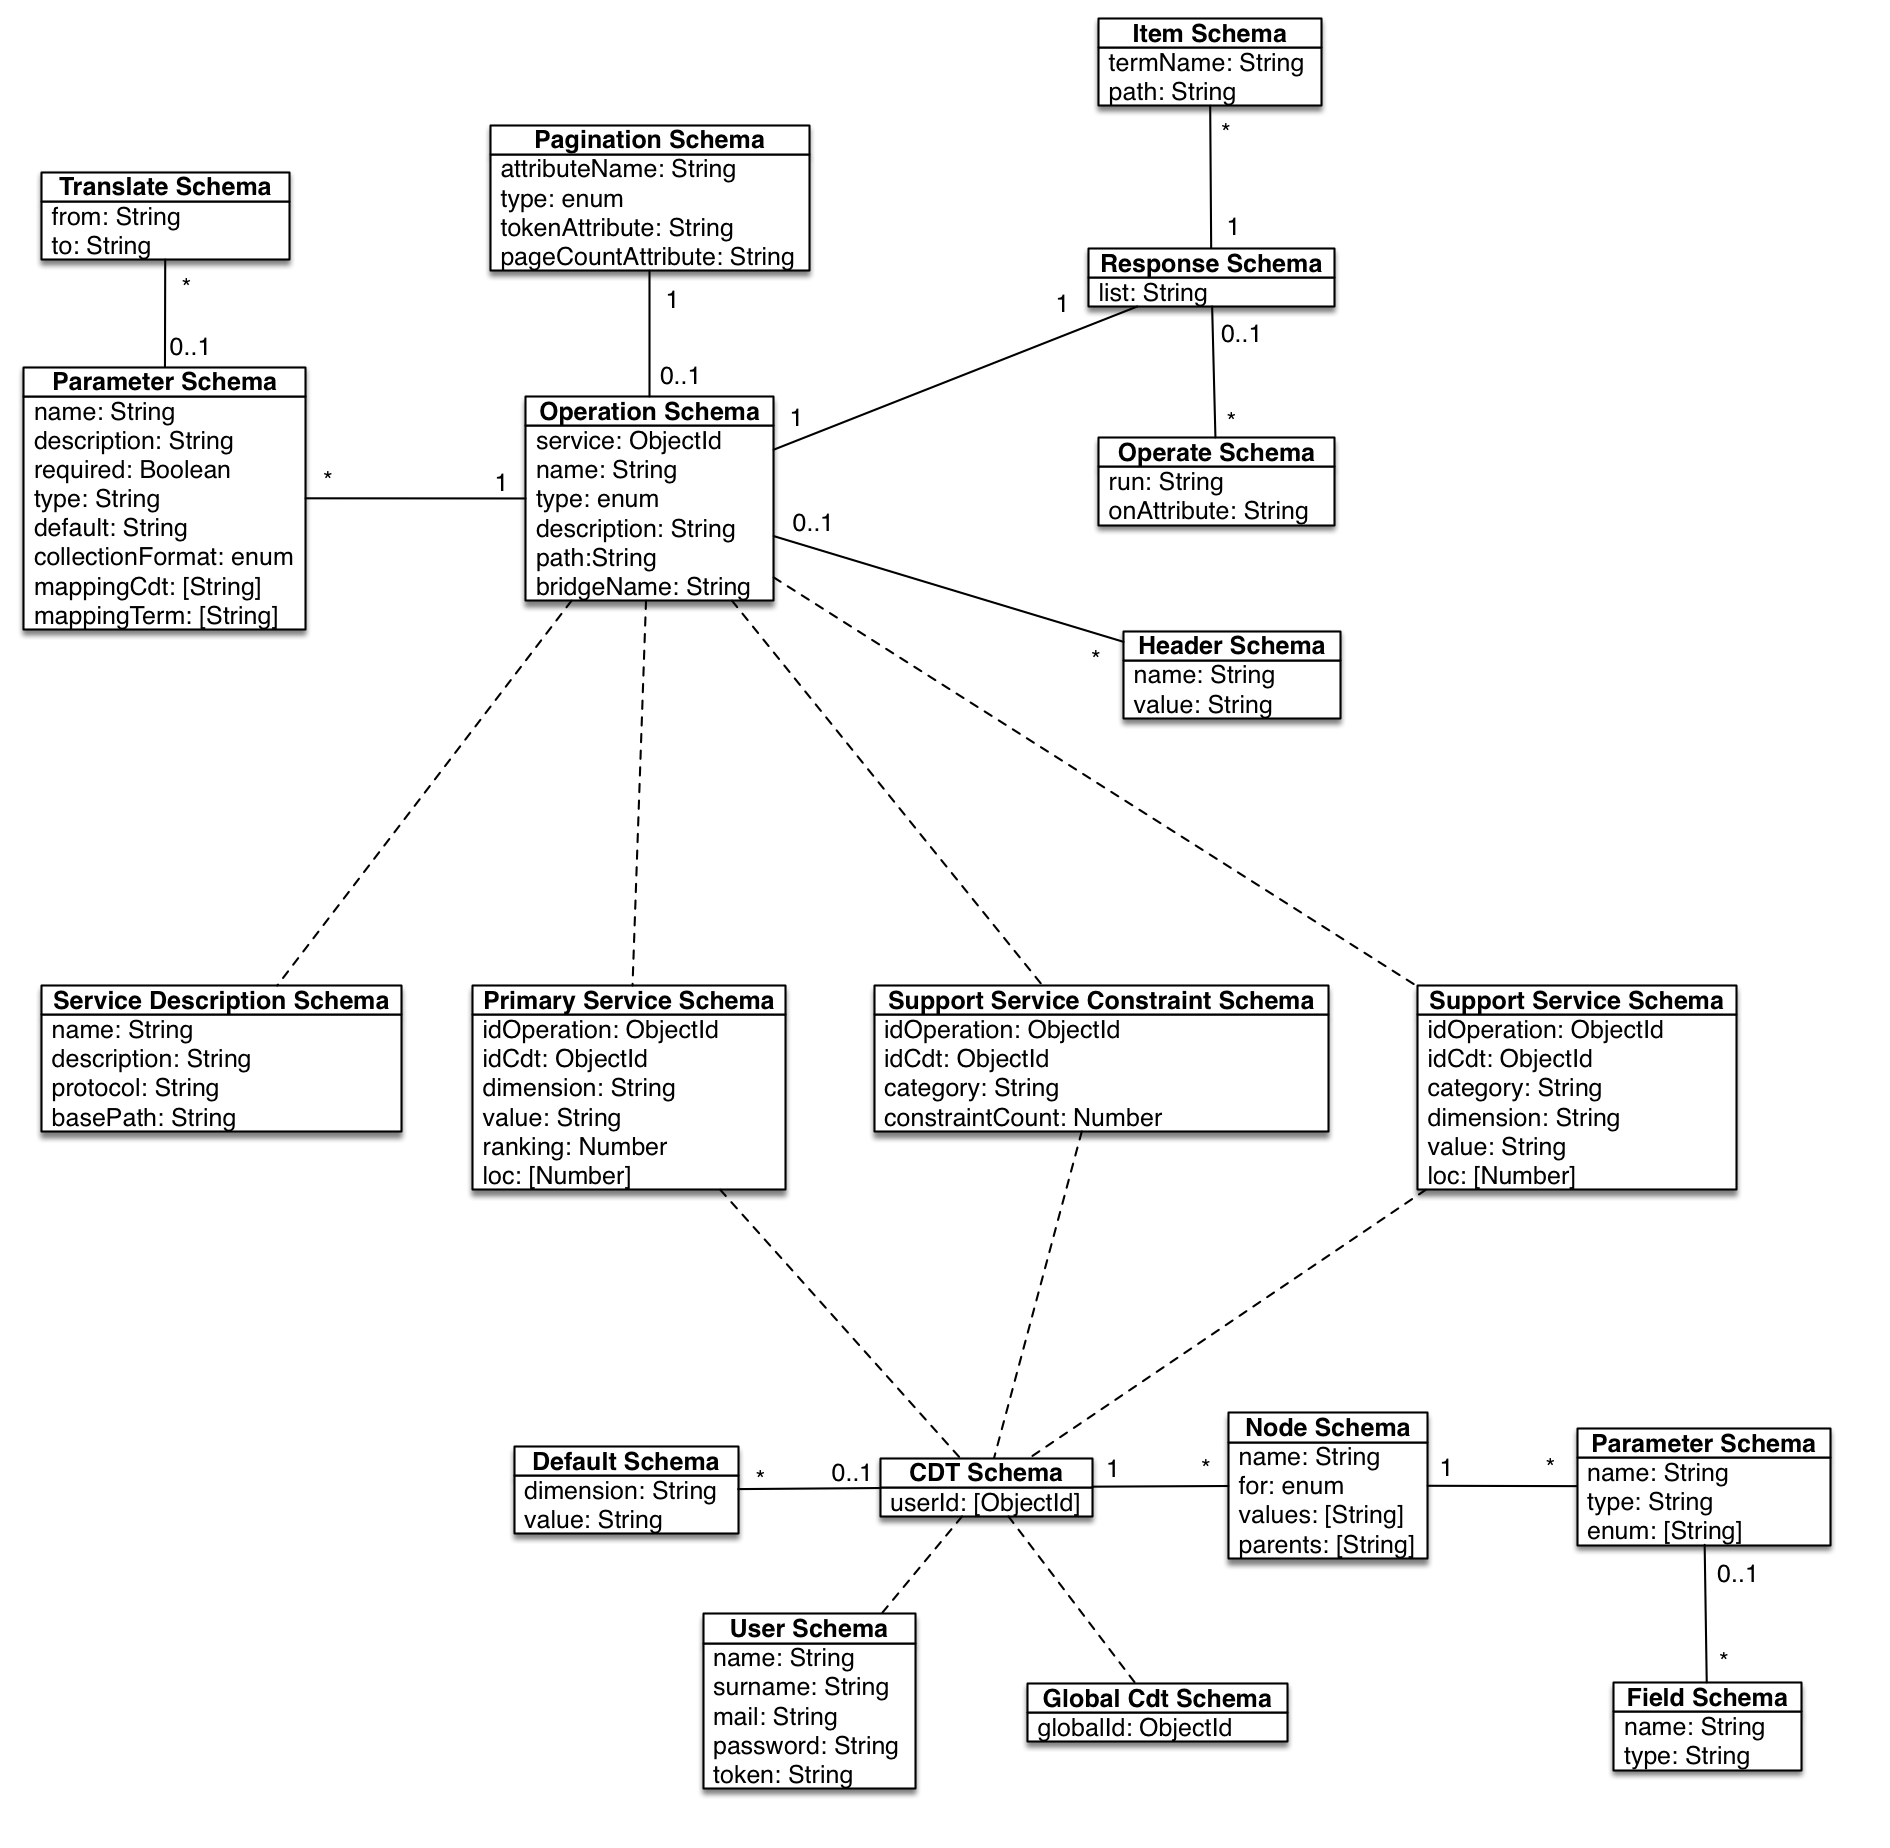
\includegraphics[width=\textwidth]{5-implementazione-backend/Immagini/schema_logico_db.png}
	\caption{Schema logico del database}\label{fig:schema-logico-db}
\end{figure}

\section{Componenti\label{sec:componenti-backend}}

Come gi� evidenziato nella Sezione \ref{sec:architettura-backend}, l'architettura del backend � composta da diversi \emph{componenti}. Questa soluzione � stata preferita per via dell'elevata flessibilit� che garantisce. Ogni componente � specializzato in un compito preciso e il concatenamento di pi� componenti fornisce il risultato desiderato. Per svolgere le principali attivit� vengono dunque create delle \emph{pipeline}, dove l'output di un componente corrisponde all'input del successivo.

Altra caratteristica importante � l'assenza di informazioni sullo stato in ogni componente. Una richiesta nasce nel momento in cui l'utente conferma l'attivit� e muore una volta che viene evasa. La ragione principale di questa scelta risiede nel fatto che sarebbe oneroso lato backend gestire tutte le informazioni della moltitudine di utenti che sono connessi al sistema. Inoltre, mantenere uno stato limiterebbe la scalabilit� del sistema, in quanto se un utente inizia la sessione su di un determinato server dovr� continuare sempre su quello, rendendo complicato il bilanciamento dei carichi tra le diverse macchine.

A questo punto � necessaria una importante precisazione: per la gestione della paginazione � necessario l'utilizzo di alcune informazioni sullo stato. Questa affermazione pu� sembrare un controsenso rispetto a ci� che � stato esposto nel paragrafo precedente. \upe dunque essenziale definire in modo dettagliato cosa si intende per \emph{stato}. La principale differenza consiste nel \emph{dove} vengono salvate le informazioni. Nel paragrafo precedente, ogni volta che si menzionava il concetto di \emph{stato}, si intendeva tutte le informazioni relative l'utente salvate all'\emph{interno} dei componenti, sotto forma di variabile. Questa soluzione, come gi� affermato anche in precedenza, risulta in un collo di bottiglia non indifferente, in quanto tutte le richieste che nascono in una determinata macchina dovranno essere gestite unicamente da essa. Si � adottata quindi una soluzione differente: i \emph{componenti} non mantengono al loro interno alcuna informazioni riguardo lo stato che a loro volta verranno memorizzate e rese disponibili da un servizio esterno. Questa soluzione permette a tutti i componenti che ne hanno esigenza di andare a recuperare le informazioni sullo stato, senza per� limitare la scalabilit� del sistema. Questo servizio pu� a sua volta offrire dei sistemi di \emph{clustering} per aumentare le perfomance in situazioni di carico elevato.

In CAMUS questa attivit� viene svolta da Redis, che � stato selezionato per l'elevata rapidit� nell'evadere le richieste e nella possibilit� di associare un tempo di vita alle informazioni che vengono memorizzate. Viene ipotizzato che dopo un determinato periodo di tempo se l'utente non effettua pi� interazione sulla sessione, essa pu� ritenersi estinta e i suoi dati eliminati.

In Figura \ref{fig:class-diagram-backend} viene mostrato il diagramma delle classi di tutti i componenti che formano il backend del sistema.

\begin{figure}[ht]
	\hspace*{-2.2cm}
	\centering
	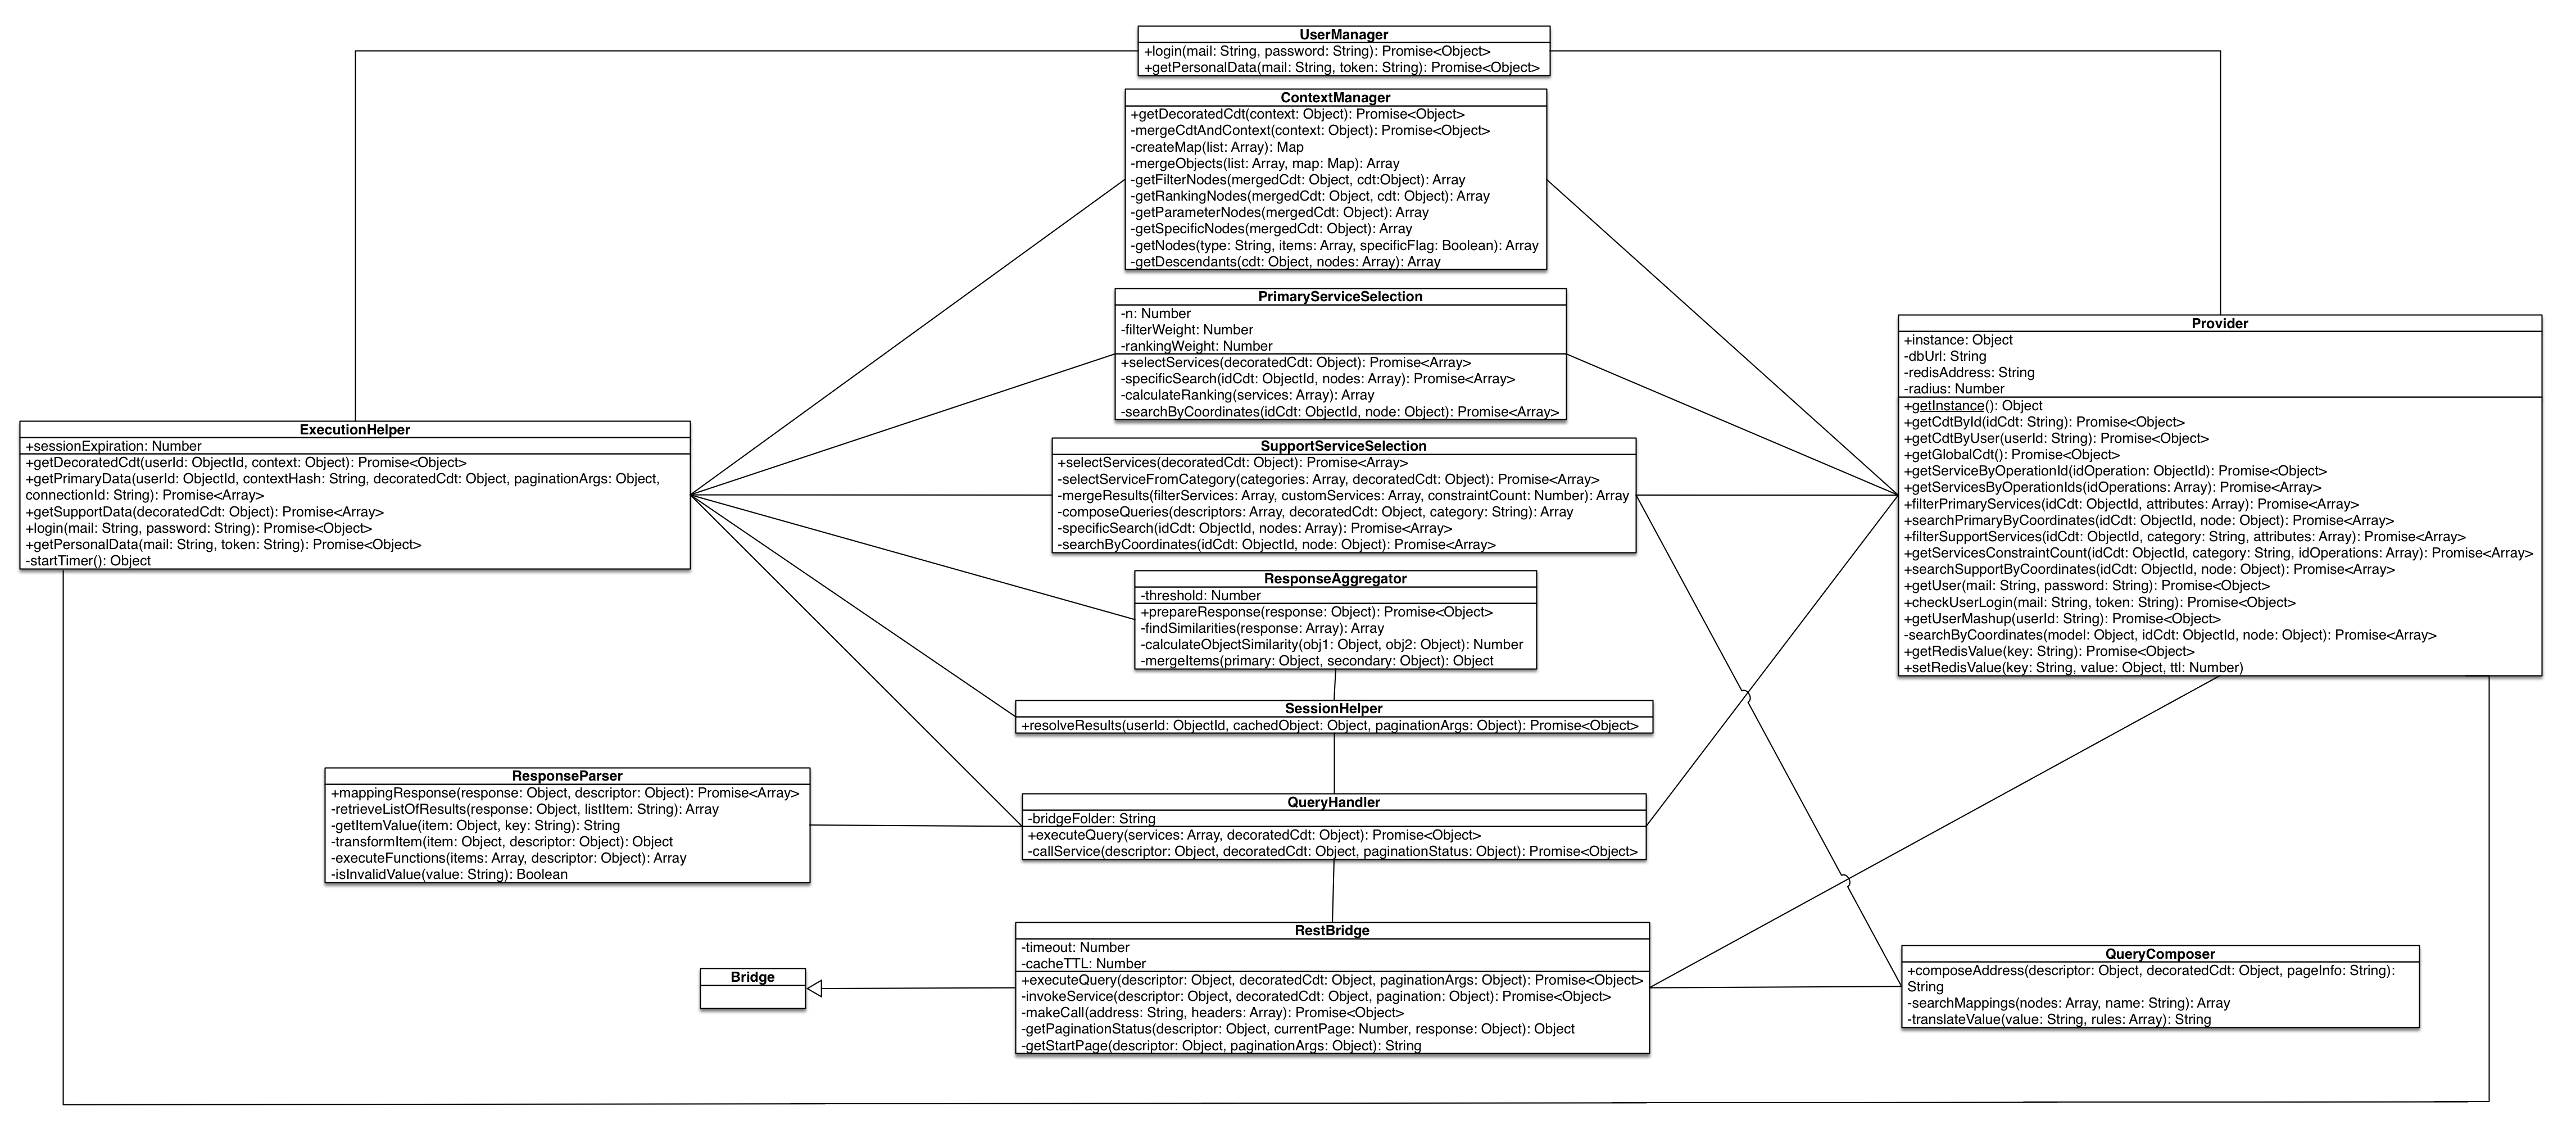
\includegraphics[width=1.4\textwidth]{5-implementazione-backend/Immagini/diagramma_classi_backend.png}
	\caption{Diagramma delle classi del backend}\label{fig:class-diagram-backend}
\end{figure}

Nelle seguenti sezioni verranno analizzate nel dettaglio le attivit� svolte dai singoli componenti.

\subsection{Provider}

Il \emph{Provider} rappresenta il punto di accesso ai database. Segue il pattern \emph{singleton}, che prevede una singola istanza della classe in comune per tutti i componenti. Le varie classi che necessitano di accedere al database possono recuperare l'istanza corrente tramite il metodo statico \emph{getInstance()}. Durante l'inizializzazione si occupa di creare le connessioni verso MongoDB e Redis. Implementa tutti i metodi necessari per recuperare le informazioni dal database e centralizza le query tutte in un singolo punto, in modo che gli altri componenti del sistema non debbano preoccuparsi di comporre le clausole. Inoltre, visto che diversi metodi vengono utilizzati da pi� componenti, si evitano duplicazioni di codice, che provoca una riduzione della manutenibilit� del sistema in quanto una modifica ad un metodo dovrebbe essere ripetuta pi� volte.

I metodi sono stati raggruppati in sei categorie, in base alla funzionalit�:

\begin{enumerate}
	\item \textbf{CDT Methods} Mette a disposizione le funzioni necessarie a recuperare gli alberi di contesto
	\item \textbf{Service Descriptor Methods} Definisce le funzioni che vengono utilizzate per acquisire i descrittori dei servizi
	\item \textbf{Primary Service Methods} Fornisce le funzioni di ricerca delle associazioni tra i nodi del CDT e le operazioni primarie
	\item \textbf{Support Service Methods} Implementa i metodi di ricerca delle associazioni tra i nodi del CDT e le operazioni di supporto
	\item \textbf{User Methods} Definisce i metodi che vengono utilizzati per l'autenticazione degli utenti e il recupero delle informazioni personali, quali il proprio \emph{albero di contesto} o i \emph{mashup}
	\item \textbf{Redis Methods} Vengono messi a disposizione i metodi per richiedere o salvare un oggetto in Redis in base alla chiave che si desidera utilizzare
\end{enumerate}

\subsection{Context Manager\label{sec:context-manager}}

Il \emph{Context Manager} � il componente dedicato alla gestione del contesto. Riceve come input il contesto dell'utente, composto dalle coppie $ {<}dimensione, valore{>} $ relative il proprio albero di contesto. La prima attivit� svolta � quella di \emph{unire} il contesto dell'utente e la descrizione del CDT presente nel database. Per unione si intende associare alla rispettiva dimensione il relativo valore ricevuto.

In seguito inizia la fase di creazione del \emph{CDT decorato}. Questa rappresentazione sar� quella che verr� utilizzata da tutti i componenti che seguono il \emph{Context Manager} nella pipeline. Il \emph{CDT decorato} non � altro che il descrittore del CDT in una forma pi� comoda per essere utilizzata nelle elaborazioni, in quanto cataloga i nodi dell'albero in quattro categorie ben specifiche, che potranno essere semplicemente recuperate dai componenti che ne hanno bisogno senza la necessit� di andare ogni volta a leggere l'intero contesto. In particolare, il CDT decorato � composto dalle seguenti categorie:

\begin{itemize}
	\item \textbf{Filter Nodes} Sono i nodi di tipo filtro che vengono utilizzati per selezionare le operazioni
	\item \textbf{Ranking Nodes} L'elenco dei nodi di tipo ranking che vengono utilizzati per selezionare le operazioni
	\item \textbf{Specific Nodes} Sono i nodi che non utilizzano la ricerca standard delle associazioni ma richiedono una ricerca specifica
	\item \textbf{Parameter Nodes} L'elenco dei nodi dai quali recuperare i valori da utilizzare per la composizione delle query
\end{itemize}

\upe da tenere in considerazione, come precedentemente fatto notare nella Sezione \ref{sec:descrittore-albero-contesto}, che alcuni nodi possono appartenere a pi� categorie nello stesso tempo. Questa eventualit� capita spesso per i nodi che vengono utilizzati sia per filtrare i servizi sia come parametro nella fase di composizione delle query.

\subsection{Primary Service Selection\label{sec:primary-service-selection}}

Il \emph{Primary Service Selection} � il componente dedicato alla ricerca delle operazioni da interrogare. Riceve come input il \emph{CDT Decorato} e produce in uscita l'elenco degli \emph{identificativi delle operazioni} selezionati, assieme al relativo \emph{punteggio}.

La prima attivit� svolta riguarda l'acquisizione delle operazioni che sono associate al contesto corrente. Questa fase viene divisa in due fasi:

\begin{enumerate}
	\item \textbf{Ricerca Standard} Viene effettuata cercando nel database tutte le operazioni che sono associate alle coppie $ {<}dimensione, valore{>} $ attive
	\item \textbf{Ricerca Specifica} Utilizza dei metodi specifici per ricercare le associazioni. Un esempio � la ricerca delle operazioni tramite \emph{coordinate}, che sfrutta le funzionalit� di MongoDB di effettuare query geospaziali
\end{enumerate}

I risultati della \emph{ricerca standard} vengono a loro volta divisi in base alla tipologia di nodo alla quale sono associati. Le due categorie sono \emph{filter} e \emph{ranking}, alle quali viene assegnato un peso diverso come descritto nella Sezione \ref{sec:selezione-operazioni}. Invece i risultati delle ricerche specifiche vengono classificati sempre come \emph{ranking}.

Una volta acquisite le associazioni attive, viene calcolato il \emph{punteggio} di ogni operazione. Viene utilizzata la Formula \ref{eq:primary-service-formula} per il calcolo del \emph{punteggio} totale di ogni operazione.

Completata questa fase, l'elenco delle operazioni viene riordinato in modo decrescente in base al \emph{punteggio} calcolato e vengono selezionate solamente le Top-N operazioni col punteggio pi� elevato. 

\subsection{Query Handler}

Il \emph{Query Handler} � il componente che orchestra le chiamate verso i servizi primari, riceve le risposte e le trasforma nel formato interno. Riceve come input gli identificativi dei servizi e ne acquisisce i descrittori completi dal database.

Una volta che sono disponibili pu� iniziare la fase di richiesta delle informazioni. Per svolgere questo compito vengono utilizzati diversi \emph{bridge}. \upe possibile cos� separare l'implementazione specifica del servizio in un altro componente, in modo che pi� servizi che condividano la medesima logica possano utilizzare lo stesso bridge. Il \emph{Query Handler} seleziona dunque il bridge idoneo per interrogare il servizio e ne esegue il metodo \emph{executeQuery()}, che si occupa di interrogare il servizio e restituire la risposta. Oltre all'elenco dei risultati, viene restituito un oggetto contenente le informazioni sullo stato della paginazione (es.: se sono disponibili ulteriori pagine o il valore per richiamare la pagina successiva), se il servizio ne implementa uno.

Quando viene restituita una risposta provvede a \emph{trasformarla} nel formato interno, basandosi sull'utilizzo dei termini semantici da associare agli attributi che compongono la risposta.

Una volta che tutti i servizi hanno risposto e i risultati sono stati trasformati, li integra assieme, accodandoli in un unico vettore, e li restituisce in uscita, pronti per essere ulteriormente elaborati dal componente successivo.

\subsection{Bridge\label{sec:bridge}}

Un \emph{Bridge} � il componente che si occupa di gestire le chiamate verso i servizi esterni e ricevere le risposte. \upe costituito da una classe astratta che deve essere estesa dalle implementazioni specifiche. In questo modo viene lasciata flessibilit� di estensione ogni qual volta � necessaria una logica diverso per invocare un servizio. In particolare, viene forzata l'implementazione del metodo \emph{executeQuery()}, che riceve come input il \emph{CDT Decorato} per recuperare i valori definiti dall'utente.

Nella sottosezione seguente viene analizzata l'unica implementazione specifica che viene fornita in dotazione col sistema, quella per l'utilizzo dei servizi di tipo REST.

\subsubsection*{REST Bridge}

Il \emph{REST Bridge} fornisce la logica per interrogare i servizi di tipo REST. La prima attivit� che svolge � la composizione dell'indirizzo verso il quale il servizio pu� essere interrogato. Viene utilizzato a tal scopo il \emph{descrittore del servizio}, che definisce i campi necessari per comporre l'indirizzo e dove andare a recuperare i valori da utilizzare. In questa fase entra in gioco anche l'informazione sulla prima pagina da interrogare, nel caso quella corrente non sia la prima chiamata che viene effettuata verso il servizio.

Una volta composto l'indirizzo completo, viene effettuata la chiamata verso il servizio. Le risposte ricevute vengono salvate in cache, quindi questa attivit� ha due varianti: se il dato � presente in cache, questo viene recuperato e fornito in uscita, altrimenti viene interrogato il servizio e il risultato fornito viene salvato in cache per utilizzi futuri.

Se il servizio prevede l'utilizza della paginazione, viene analizzata la risposta alla ricerca di informazioni sulla presenza di ulteriori pagine da richiedere. In particolare vengono cercati gli attributi relativi al numero totale di pagine o al token per richiamare la pagina successiva, in base alla tipologia implementata dal servizio.

Infine, viene restituito in uscita la risposta del servizio insieme alle eventuali informazioni riguardo la paginazione, che in particolare sono due: \emph{i)} hasNextPage, che indica se � presente un'altra pagina; \emph{ii)} nextPage, che specifica il numero di pagina o token da utilizzare per richiamare la nuova pagina.

\subsection{Response Aggregator}

Il \emph{Response Aggregator} entra in gioco una volta che sono stati interrogati tutti i servizi. Riceve in input l'elenco dei risultati gi� trasformati. Il suo compito � di effettuare diverse attivit� per pulire i dati o aggiungere ulteriori informazioni. Al momento, nel prototipo viene eseguita unicamente la \emph{ricerca dei duplicati}. Questa attivit� scorre l'intera lista dei risultati e cerca gli oggetti che sono simili tra loro, cio� che rappresentano la medesima entit� reale. Ogni qualvolta che due o pi� oggetti vengono identificati come duplicati, viene avviata un'attivit� per unirli in un unico oggetto. Questo oggetto conterr� l'unione delle informazioni che ognuno degli elementi mette a disposizione. In questo modo � possibile creare un entit� pi� ricca rispetto a quelle originali. Nel caso in cui ci sia sovrapposizione, ossia quando due o pi� entit� forniscono lo stesso attributo, viene mantenuto il valore restituito dal servizio col punteggio pi� alto, che si ipotizza sia quello che mette a disposizione i migliori dati per la situazione corrente. Per un'analisi pi� approfondita dell'algoritmo di ricerca dei duplicati si fa riferimento all'Algoritmo \ref{alg:algoritmo-rimozione-duplicati}.

Un'ulteriore attivit�, che non � ancora stata implementata, riguarda l'assegnamento di un \emph{punteggio} ad ogni elemento, in base alle informazioni di contesto disponibili. Per esempio, sar� possibile assegnare un punteggio pi� alto all'elemento che si trova pi� vicino rispetto all'utente e, per gli altri elementi, verr� assegnato un punteggio via via decrescente man mano che ci si allontana dal punto di riferimento. Si stanno prendendo in considerazione anche logiche di \emph{selezione fuzzy} per permettere una flessibilit� maggiore nell'assegnare i vari punteggi.

Una volta terminate le attivit� sui dati, viene restituita la nuova lista dei risultati.

\subsection{Support Service Selection}

Il \emph{Support Service Selection} � il componente dedicato alla selezione delle operazioni di supporto o intent. Riceve in ingresso il \emph{CDT Decorato} che, oltre a contenere le selezioni fatte dall'utente, elenca anche le categorie di servizi che si desidera ricevere. Le categorie servono per raggruppare pi� servizi che svolgono una funzione simile assieme. In base alle associazioni definite verr� poi selezionato il servizio pi� idoneo per la situazione corrente. L'attivit� di selezione che viene descritta � ripetuta integralmente per ognuna delle categorie, in quanto si vuole ottenere almeno un riscontro per tutte le categorie elencate. Come nel caso delle operazioni primarie, si inizia con la ricerca delle operazioni associate ai nodi attivi del CDT. In questo caso non viene pi� fatta la divisione tra nodi di tipo \emph{filter} e nodi di tipo \emph{ranking} bens� vengono unite queste due categorie. Invece viene mantenuta la logica di ricerca delle associazioni che richiedono dei metodi specifici. Come gi� descritto nella Sezione \ref{sec:selezione-operazioni}, per le operazioni di supporto le associazioni vengono intese pi� come \emph{vincoli}. A questo scopo vengono contestualmente recuperati il numero di vincoli associati alle operazioni per le quali � stata trovata almeno un'associazione. Questo passaggio � essenziale, in quanto si vogliono effettivamente selezionare solamente le operazioni che hanno un numero di vincoli uguale o maggiore di quello preimpostato. Il caso in cui i conteggi siano pari � intuitivo, mentre richiede una spiegazione il fatto che esistano situazioni nelle quali il conteggio sia maggiore rispetto al numero di vincoli. Si prenda come esempio un servizio dei trasporti che espone una operazione. Questa operazione necessita di un parametro che specifica se si preferisce spostarsi col \emph{bus} o con la \emph{metro}. Questo valore viene dunque recuperato dall'albero di contesto, in base alla selezione effettuata dall'utente. Visto che si tratta di una sola operazione, ma � valida per pi� situazioni, verr� associata a due diversi nodi dell'albero. Il conteggio dei vincoli dovr� invece rimanere pari a uno, come se si fosse effettuata una singola associazione. Infatti non � possibile inserire come valore due, perch� altrimenti l'operazione non verrebbe mai selezionata, in quanto risulterebbe una sola associazione.

Una volta che sono state selezionate le operazioni che rispettano il numero di vincoli associato, vengono mantenute solamente le operazioni che hanno il numero massimo di vincoli. La ragione di questa scelta � dovuta al fatto che pi� vincoli sono rispettati vuol dire che l'operazione � pi� attinente al contesto.

L'ultimo passaggio riguarda la composizione degli indirizzi delle operazioni selezionate. In seguito l'elenco creato viene restituito in uscita, in modo che sia utilizzabile dall'app mobile.

\subsection{Session Helper}

Il \emph{Sessione Helper} viene utilizzato quando � stata effettuata una prima richiesta ai servizi e l'app mobile richiede ulteriori dati. Si occupa di gestire il salvataggio in cache della sessione ed eventualmente, quando il primo result set sta per terminare, richiama un'altra volta i servizi richiedendo la pagina successiva.

Per gestire la paginazione tra backend e app mobile vengono utilizzati due parametri:

\begin{itemize}
	\item \textbf{First} Questo campo specifica il numero di elementi che vengono richiesti
	\item \textbf{After} Definisce il \emph{cursore} di partenza. Verranno quindi restituiti il numero di elementi specificati nell'attributo \virgolette{first} dopo l'elemento con quello specifico identificatore
\end{itemize}

La prima attivit� che viene eseguita � tenere traccia di quanti elementi sono stati visualizzati dall'utente. Questa informazione � necessaria per conoscere quanti elementi rimangono ancora da visualizzare. A questo punto viene controllato se sono disponibili abbastanza informazioni da mostrare, tramite la formula:

\begin{equation}
	elementi\_mostrati \le totale\_elementi - first - 1
\end{equation}

Dove:

\begin{itemize}
	\item \textbf{elementi\_mostrati} indica il numero di elementi che sono gi� stati mostrati all'utente
	\item \textbf{totale\_elementi} rappresenta il numero totale di elementi presenti in cache
	\item \textbf{first} � lo stesso attributo descritto in precedenza, che indica quanti elementi sono stati richiesti
\end{itemize}

Se l'equazione � rispettata vengono semplicemente restituiti i dati presenti in cache, altrimenti il \emph{Session Helper} si occupa di recuperare dalla cache le informazioni sui servizi prescelti nella richiesta originale e sulle pagine da richiedere ed effettua le richieste ai servizi, sfruttando in particolari il \emph{Query Handler} ed il \emph{Response Aggregator}.

\section{Endpoint GraphQL}

\textcolor{red}{Mostrare quali endpoint sono stati realizzati\\
	Accennare alcuni dettagli sul come sono stati realizzati gli schemi GraphQL\\
	Descrivere vantaggi e problematiche}

\section{Flusso di una richiesta\label{sec:flusso-richiesta-server}}

\textcolor{red}{mostrare come viene elaborata una richiesta proveniente dalla mobile app\\
	mostrare diagramma di flusso delle scelte se andare a recuperare il dato in cache o fare un nuova richiesta, e se in cache se � necessario reinterrogare il servizio\\
	mostare flusso di una nuova richiesta\\
	mostrare flusso di una richiesta che richiede dati dai servizi e li aggiunge a quelli gi� presenti in cache}

\begin{figure}[ht]
	\centering
	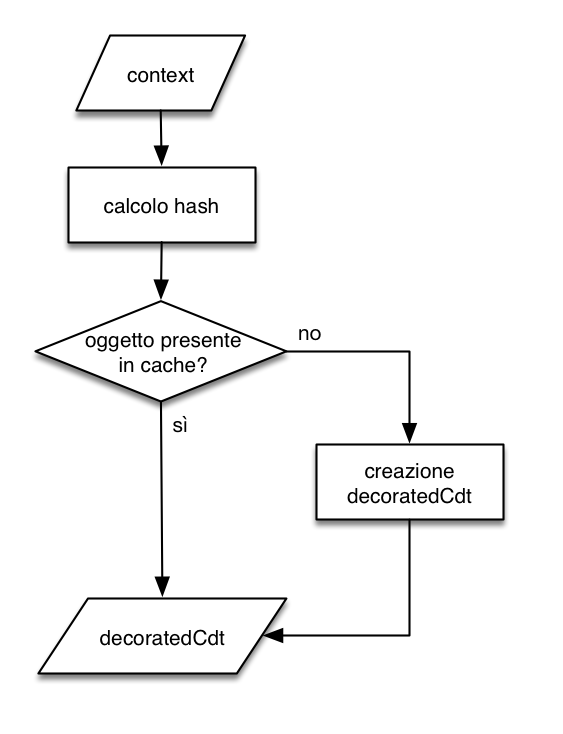
\includegraphics[width=0.43\textwidth]{5-implementazione-backend/Immagini/diagramma_flusso_decoratedCdt.png}
	\caption{Flusso di creazione del CDT decorato\label{fig:flusso-decorated-cdt}}
\end{figure}

\begin{figure}[ht]
	\centering
	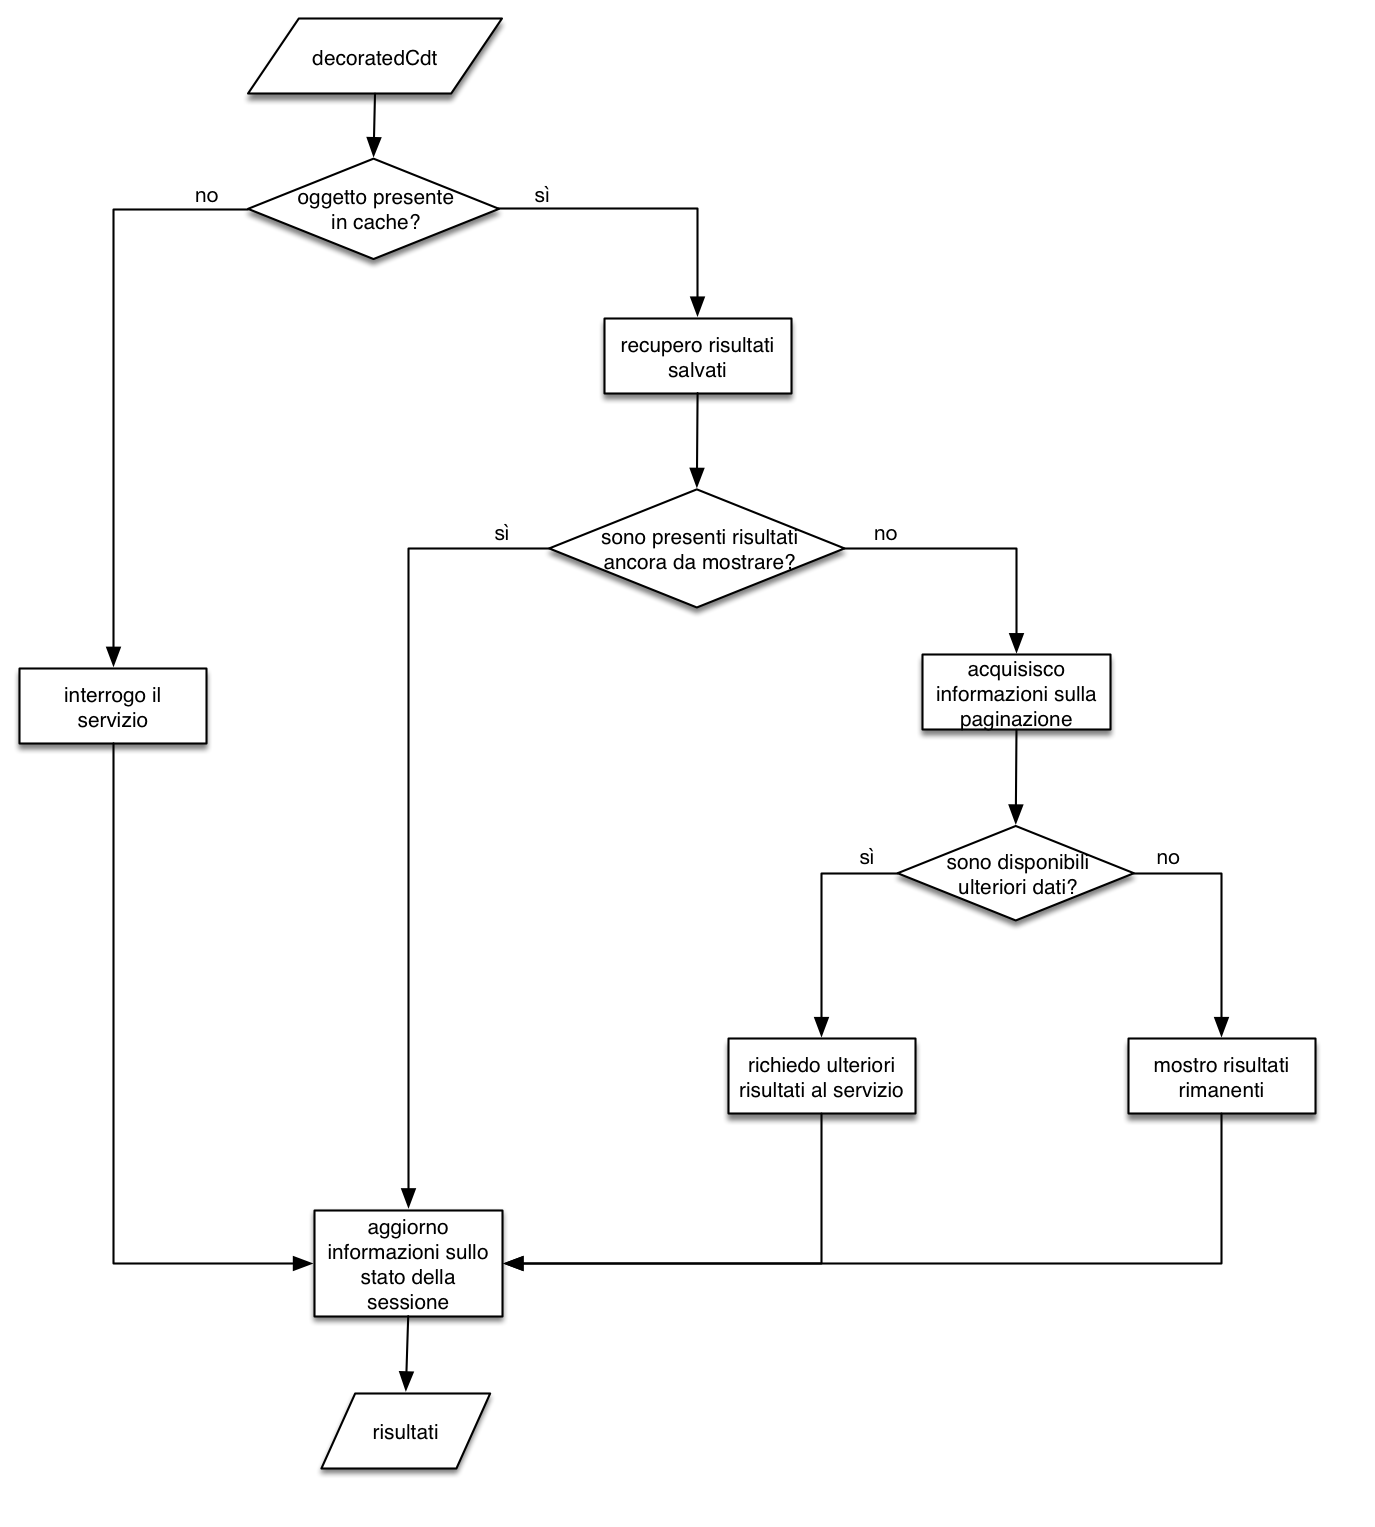
\includegraphics[width=\textwidth]{5-implementazione-backend/Immagini/diagramma_flusso_servizi_primari.png}
	\caption{Flusso di richiesta dei risultati primari\label{fig:flusso-servizi-primari}}
\end{figure}
	
\begin{figure}[ht]
	\centering
	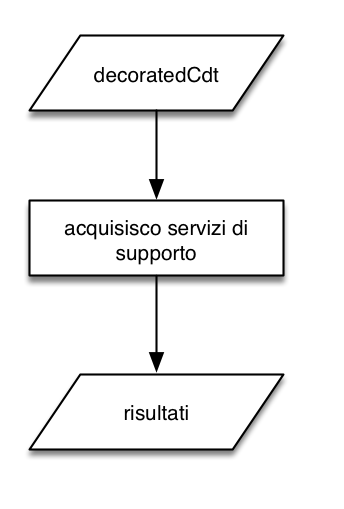
\includegraphics[width=0.3\textwidth]{5-implementazione-backend/Immagini/diagramma_flusso_servizi_supporto.png}
	\caption{Flusso di richiesta dei risultati di supporto\label{fig:flusso-servizi-supporto}}
\end{figure}

\section{File di configurazione}

\textcolor{red}{Spiegare campi del file di configurazione e variabili d'ambiente\\
	Nomi dei file per i vari ambienti (sviluppo, produzione)}


\chapter{Progettazione di dettaglio e implementazione della mobile app\label{ch:implementazione-app}}

L'applicazione \emph{mobile} CAMUS rappresenta l'altro elemento fondamentale dell'ar\-chi\-tet\-tu\-ra. Fornisce all'utente finale l'interfaccia per accedere al sistema e semplifica l'utilizzo e l'accesso ai dati. Il capitolo si apre con una descrizione dettagliata delle \emph{Actions} e delle \emph{Stores} di \emph{Alt.js}.
%
Successivamente viene introdotto lo schema per definire le pagine e la logica di aggiornamento dei dati, seguendo il principio del flusso dati unidirezionale. In seguito viene definita la struttura del file di \emph{mashup} proveniente dal \emph{server}, che è indispensabile per la creazione delle schermate dell'app, per poi trattare nello specifico i metodi necessari per la costruzione di queste schermate.
Successivamente si illustra il flusso dei dati all'interno dell'applicazione e di come vengono gestite le richieste dati verso il \emph{server}, tramite GraphQL, per effettuare le attività riguardanti il \emph{login} e la ricerca delle informazioni contestuali per l'utente. In conclusione verrà trattato l'argomento riguardante i servizi di supporto.

\section{Gestione dello stato}\label{sec:state-management}
In questa sezione sono descritte nel dettaglio tutte le \emph{Actions} e le \emph{Stores} utilizzate nell'applicazione e presentate nella Sezione \ref{sec:action-store}

\subsection{Actions\label{sec:actions}}

Le \emph{Actions} sono i metodi utilizzati per modificare lo stato dell'ap\-pli\-ca\-zio\-ne. Vengono utilizzate principalmente in due modi:

\begin{itemize}
	\item \textbf{Data Fetching}
	Quando è necessario scaricare gli elementi necessari per il corretto funzionamento dell'applicazione (CDT e \emph{mashup}) o i dati provenienti dalle richieste, le \emph{action} hanno lo scopo di modificare lo stato per cambiare la \emph{view} dell'applicazione a seconda dello stato della richiesta.
	Per esempio, quando si preme il pulsante per effettuare una nuova richiesta basata sul contesto, viene invocata un'azione per mantenere lo stato coerente tra più componenti e permettere di mostrare in fase di caricamento uno \emph{Spinner}. Una volta che la richiesta viene evasa e i dati sono disponibili, viene eseguita un’altra azione per mostrarli all’interno di una \emph{ListView}
	\item \textbf{Application State}
	Lo stato generale dell'applicazione viene salvato utilizzando delle \emph{Action} chiamate dalle interazioni dell'utente con l'interfaccia grafica. Per esempio quando viene composto il contesto le diverse selezioni sono passate dall'utente tramite le \emph{Context Actions} nelle \emph{Context Store}, per poi rimanere disponibili per la visualizzazione delle selezioni già effettuate o la costruzione della \emph{query} per i dati
\end{itemize}	

Le \emph{Actions} implementate nell'applicazione sono le seguenti:

\begin{itemize}
	\item \textbf{User Actions}
	Sono le azioni che servono ad aggiornare i parametri relativi all'utente, come \emph{password}, \emph{email} e il suo identificativo della sessione:
	\begin{itemize}
		\item \textbf{Update Email}
		Metodo per aggiornare l'\emph{email} dell'utente 
		\item \textbf{Update Password}
		Metodo per aggiornare la \emph{password} dell'utente
		\item \textbf{Update Token}
		Metodo per tenere in memoria il \emph{token} della connessione col \emph{server}
	\end{itemize}
	\item \textbf{Context Actions}
	Sono le azioni che gestiscono la selezione del contesto, consentendo di modificare le scelte effettuate dall'utente:
	\begin{itemize}
		\item \textbf{Set Transport}
		Metodo per salvare la tipologia di trasporto da parte dell'utente
		\item \textbf{Set Typology}
		Metodo per salvare la tipologia nel caso di trasporto non con mezzi propri
		\item \textbf{Add Forbidden}
		Metodo per aggiungere un parametro in quelli da nascondere all'utente
		\item \textbf{Remove Forbidden}
		Metodo per rimuovere il parametro selezionato dalla lista di quelli da nascondere all'utente
		\item \textbf{Update Last Context}
		Metodo per salvare l'ultimo contesto inviato al \emph{server}, per poterlo riutilizzare nelle richieste per le pagine successive
	\end{itemize}
	\item \textbf{View Actions}
	Sono le azioni relative alla gestione dei \emph{mashup} ma non dello stato della navigazione, per le quali è utilizzato un componente aggiuntivo sempre basato su Flux (React Native Router Flux):
	\begin{itemize}
		\item \textbf{Set Views}
		Metodo per salvare il file con le \emph{view} provenienti dal \emph{server} 
		\item \textbf{Select Interest Topic}
		Metodo per salvare l'\emph{Interest Topic} selezionato dall'utente. Questa funzione è chiamata quando nella pagina iniziale l'utente seleziona l'\emph{Interest Topic} per la selezione della \emph{view} appropriata
	\end{itemize}
	
	\item \textbf{Data Actions}
	Trattano della gestione del CDT e dei risultati ottenuti dal \emph{server}:
	\begin{itemize}
		\item \textbf{Update Results}
		Metodo per aggiornare i dati dei risultati provenienti dalla \emph{query} basata sul contesto
		\item \textbf{Results Failed}
		Metodo per inviare il messaggio di errore proveniente dalla richiesta
		\item \textbf{Update Full CDT}
		Metodo per aggiornare il CDT associato all'utente
	\end{itemize}
\end{itemize}

\subsection{Stores\label{sec:stores}}

Le \emph{Stores} salvano lo stato dell'applicazione e forniscono alle \emph{view} nuovi dati ogni volta che sono aggiornate. 
Per ogni interazione sui dati dell'ap\-pli\-ca\-zio\-ne che necessitano di rimanere persistenti viene invocata una \emph{action} dal componente e dalla \emph{view} che si propaga prima nelle \emph{store} e successivamente aggiorna nuovamente la \emph{view}.
Si è scelto di suddividere le \emph{Store} per tipologia di operazione e dato trattata:

\begin{itemize}
	\item  \textbf{User Store}
	Nella \emph{User Store} sono memorizzati tutti i dati relativi all'utente. In particolare viene memorizzata la \emph{mail} dell'utente e l'identificativo del CDT a lui associato, che serviranno per poter effettuare le \emph{query} GraphQL per ottenere i dati
	\item \textbf{Context Store}
	Nel \emph{Context Store} vengono gestiti i dati che riguardano i dati di contesto, come le coordinate geografiche e le scelte delle tipologie di trasporto pubblico, in modo da essere riutilizzate. Per quanto riguarda le richieste di dati, una volta che il contesto viene composto per effettuare la prima \emph{query}, questo \emph{payload} viene salvato qui e poi riutilizzato nelle \emph{query} dei risultati successivi
	\item \textbf{View Store}
	In questa \emph{store} sono memorizzati tutti i dati relativi alle \emph{view}. Qui viene salvato lo schema di \emph{mashup} e l'\emph{Interest Topic} corrente
	\item \textbf{Data Store}
	Si tratta della \emph{store} più complessa perchè deve gestire in modo dinamico diverse tipologie di dato. Quando viene ricevuto il CDT vengono scanditi gli \emph{interest topic} è creato un oggetto nel campo \emph{results} che è composto da un \emph{array} di tanti oggetti definiti da due campi:
	\begin{enumerate}
		\item \textbf{Results}
		Rappresenta i risultati ricevuti per quell'\emph{interest topic}, comprende i dai servizi primari e i collegamenti per i servizi di supporto
		\item \textbf{Topic}
		Rappresenta l'\emph{Interest topic} associato ai risultati ricevuti dal \emph{server}
	\end{enumerate}
	Questa operazione è necessaria per poter gestire il fatto di avere comunque dei dati in memoria in condizioni di assenza di rete, anche per tipi diversi di risultati provenienti dal \emph{server} e per essere in grado di gestire una cardinalità variabile di tipologie di dati. Nel Listato \ref{lst:store-two-topics} è mostrato come viene rappresentato lo stato nel caso in cui l'utente abbia a disposizione due \emph{Interest Topic} e la suddivisione dei risultati per le due tipologie, in questo caso \emph{Restaurants} ed \emph{Event}. Si noti che oltre ai risultati sono salvati anche i parametri con lo stato della paginazione, per lasciare la possibilità di riprendere la visione di nuovi risultati.
\end{itemize}

\begin{listing}[H]
	\inputminted{json}{4-progettazione-alto-livello/Codice/store-two-topics.json}
	\caption{Esempio Data Store Mashup}
	\label{lst:store-two-topics}
\end{listing}

\section{Struttura dello schema di mashup\label{sec:struttura-schemi-mashup}}

Per poter permettere una dinamicità nella struttura delle schermate che formano l'applicazione si è scelto di utilizzare uno schema di \emph{mashup} molto semplice e allo stesso tempo in grado di fornire i parametri necessari all'applicazione per costruire le viste in tempo reale. Si è scelto di utilizzare una rappresentazione in JSON in modo da essere facilmente interpretabile all'interno del motore JavaScript di React Native. 
Nel caso di CAMUS sono considerate due tipologie di schema di \emph{mashup}: la \emph{list} e la \emph{details}. 
%cambiare questa frase 
Nella tipologia \emph{list} sono definite le \emph{view} che descrivono il singolo \emph{item} della \emph{ListView} e generalmente si compone di una quantità non eccessiva di componenti. 
Nel caso della \emph{list} sono definiti gli elementi da mostrare quando è presente la lista complessiva di risultati nella \emph{ListView}.
Nella tipologia \emph{details} sono disponibili tutti i dettagli dell'\emph{item} selezionato e sono definiti tutti i termini necessari a identificare l'elemento per l'utente.
Considerando l'esempio dei ristoranti, per la lista sono associati i termini che servono a identificare l'oggetto, come il nome e l'indirizzo. Se poi l'utente vuole vedere la mappa e visualizzare gli estremi per contattare il ristorante deve aprire la pagina dei dettagli, dove acquisendo i termini dal file di \emph{mashup}, sono visualizzati tutti i dettagli necessari per l'utente. Inoltre è specificata la tipologia dell'elemento da visualizzare, in modo da permettere all'\emph{app} di utilizzare le librerie di collegamento con le applicazioni specifiche del sistema operativo.

Nel Listato \ref{lst:mashup-schema} viene mostrato un esempio del file JSON di \emph{mashup} della pagina di dettaglio e in Figura \ref{fig:schermate-app-mashup} la sua traduzione nelle due versioni dell'applicazione.

\begin{listing}[H]
	\inputminted{json}{6-implementazione-app/Codice/mashup-schema-example-app.json}
	\caption{Esempio Schema Mashup}
	\label{lst:mashup-schema}
\end{listing}

\begin{figure}[ht]
	\begin{subfigure}{0.5\textwidth}
		\centering
		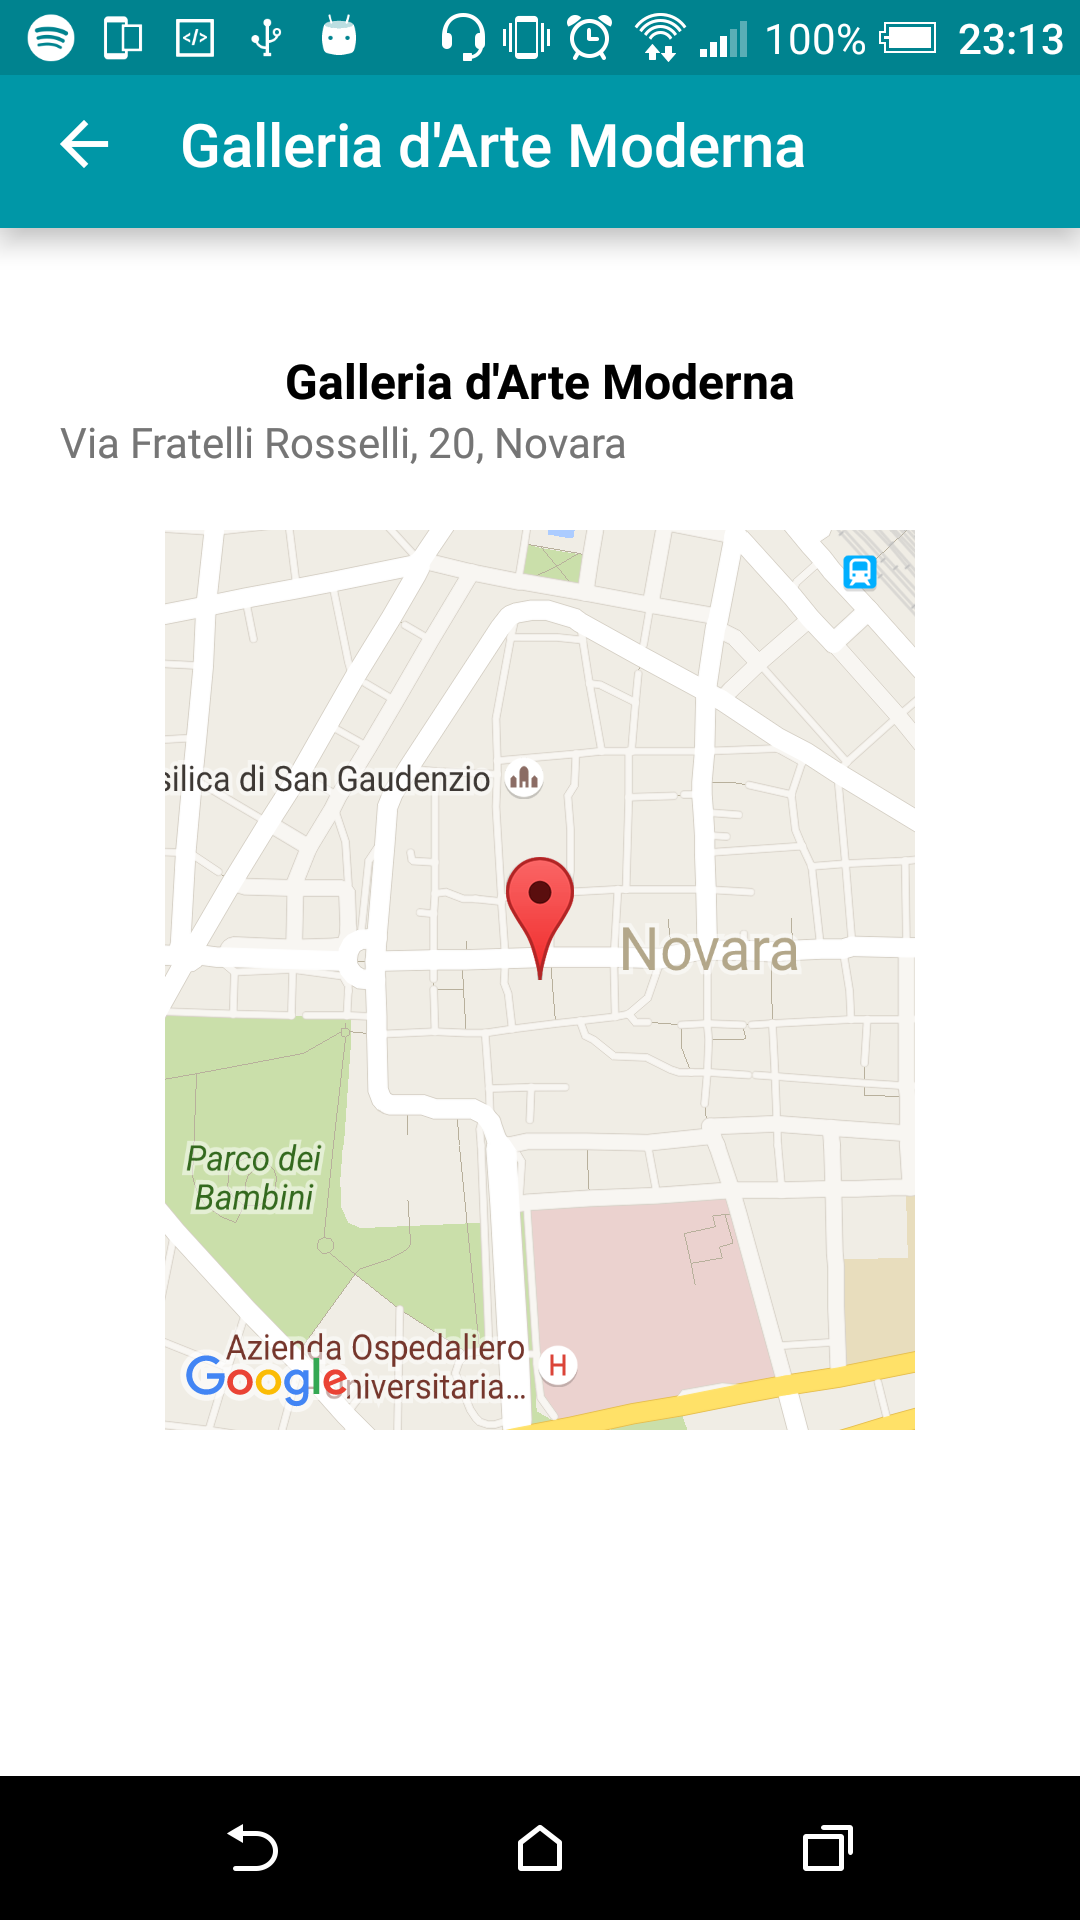
\includegraphics[width=0.48\textwidth]{6-implementazione-app/immagini/details_android.png}
		\caption{Versione Android}
	\end{subfigure}
	\begin{subfigure}{0.5\textwidth}
		\centering
		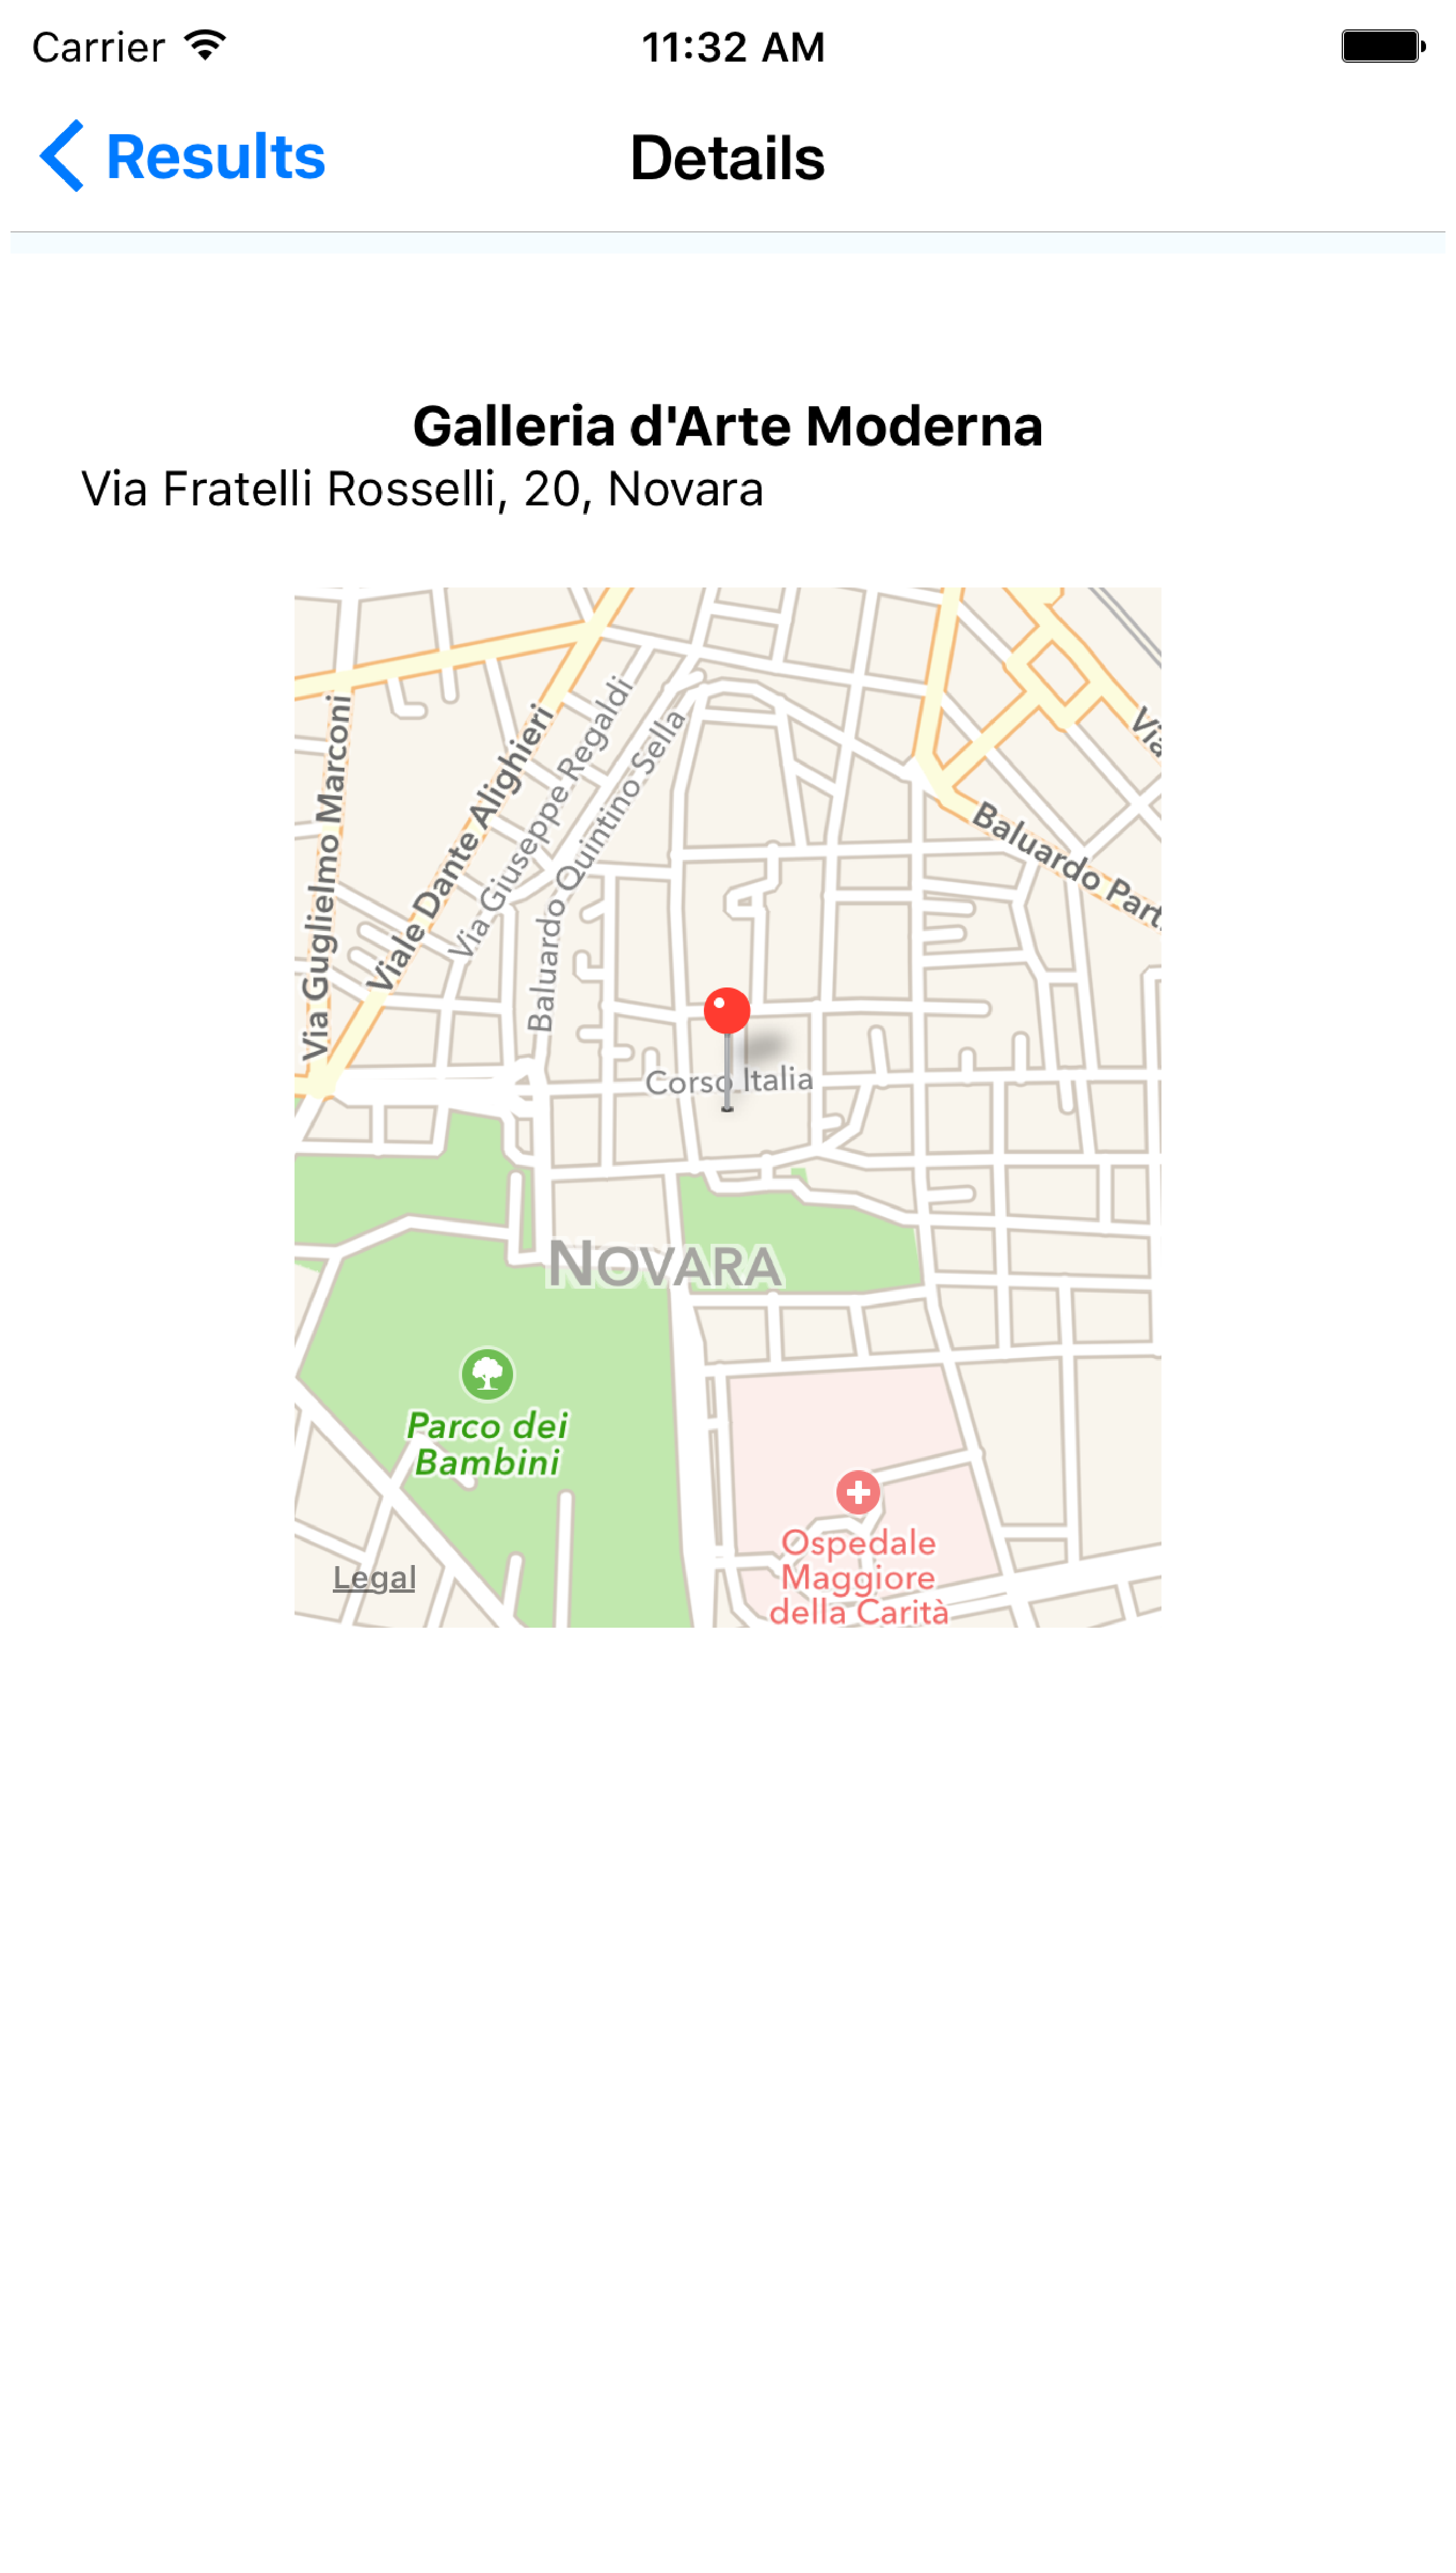
\includegraphics[width=0.48\textwidth]{6-implementazione-app/immagini/details_ios.pdf}
		\caption{Versione iOS}
	\end{subfigure}	
	\caption{Schermata dei dettagli}
	\label{fig:schermate-app-mashup}
\end{figure}

Di seguito sono elencate le diverse tipologie di dato che compongono l'oggetto che rappresenta i file di \emph{mashup}:

\begin{itemize}
	\item \textbf{Type}
	Il termine \emph{type} indica la tipologia dell'elemento da visualizzare nella \emph{view}. È associato a un componente React Native, che verrà richiamato nella fase di costruzione dell'interfaccia grafica
	\item \textbf{Topic}
	Si tratta di un \emph{array} di stringhe che indica tutte le aree di interesse associate allo schema in questione. Si è scelto di utilizzare una struttura basata su \emph{tag}: una volta che l’utente sceglie l’\emph{interest topic} viene utilizzato lo schema che lo possiede nei suoi \emph{tag} 
	\item \textbf{Contents}
	Indicano i termini del \emph{mashup} o dei nuovi componenti innestati. Se nell'oggetto padre è specificato un tipo gli elementi in \emph{contents} rappresentano i termini da richiedere nella \emph{query} GraphQL. In caso contrario questo campo indica che in \emph{contents} è presente un nuovo livello di annidamento. Ci possono essere tanti annidamenti, fino a quando non si arriva ad avere un oggetto che possiede il campo \emph{type}
	\item \textbf{Style}
	Questo campo serve per definire uno stile da assegnare al componente. Permette di personalizzare l’aspetto del componente, andando a ridefinire lo stile predefinito. Viene utilizzato Flexbox per la specifica degli stili
\end{itemize}

\section{Rendering delle view}\label{sec:rendering-view}

Si tratta della funzionalità più delicata da progettare all'interno dell'applicazione, perché non è così semplice pensare di generare in modo dinamico delle pagine con così tanta mutabilità a partire da un documento strutturato delle interfacce visuali.
Mentre in codice nativo questo problema può presentare delle difficoltà a livello implementativo, l'utilizzo da parte di React di un \emph{Virtual DOM} simile al linguaggio HTML offre il vantaggio di poter generare molto rapidamente una traduzione dal file di \emph{mashup} a un modello interpretabile dal motore di \emph{rendering} dell'\emph{app}.
Per questo motivo è stato creato un componente apposito, il \emph{View Builder}, che, dato un oggetto contenente lo schema di \emph{mashup}, riesce a gestire l'associazione dei contenuti semantici all'interno di questo schema con i componenti presenti nell'applicazione, restituendo il componente finale.
Sono presenti all'interno due tipologie di \emph{rendering}: il \emph{rendering} del contesto e il \emph{rendering} dei risultati.

\subsection{Rendering a partire dal contesto}

Il \emph{rendering} del contesto è basato esclusivamente su elementi provenienti dal CDT. Non si è reso necessario l'utilizzo di schemi di \textit{mashup}, in quanto tutti i dati occorrenti all'applicazione per costruire le \emph{view} sono già presenti all'interno del CDT. Per ogni elemento del CDT viene eseguita un'associazione a componenti già esistenti di \emph{React Native}, come per esempio \emph{Text} per mostrare il nome dell'elemento o \emph{Picker} in caso di selezioni multiple. Di seguito sono mostrati i diversi metodi di costruzione delle viste partendo dai singoli elementi del CDT:

\begin{itemize}
	\item \textbf{Interest Topic}
	Gli \emph{Interest Topic} hanno bisogno di essere selezionati nella pagina iniziale una volta effettuata l'autenticazione e caricati in una lista di pulsanti con due elementi per riga e con un'icona rappresentativa. I pulsanti e le icone sono predefinite nell'applicazione e necessitano soltanto di una associazione <\emph{nome},\emph{elemento}> dal campo \emph{Interest Topic} del CDT. Questa funzione molto semplice viene eseguita direttamente all'interno della pagina principale senza la necessità di utilizzare il \emph{View Builder}
	\item \textbf{Altri elementi}
	Gli altri elementi del contesto sono elaborati all'interno del componente \emph{View Builder}. Con una funzione ricorsiva viene scandito l'intero CDT ricevuto dal \emph{server} con i campi da modificare e in base ai contenuti viene costruito l'elemento della \emph{view}, a seconda della tipologia. Per esempio, se per un campo è richiesto l'inserimento di un numero verrà mostrato un \emph{TextInput} che permette il completamento solo con numeri, mentre se è necessario effettuare una scelta tra più elementi verrà mostrata una lista selezionabile.
	Assume una grande importanza anche la gestione delle esclusioni tra le operazioni. Se viene selezionato \virgolette{With Car} non è corretto mostrare le possibili tipologie di trasporto pubblico, perché si conosce già a priori che l'utente non selezionerà mai nello stesso momento come mezzo di trasporto l'automobile e il bus. Per questo scopo viene utilizzato il parametro \emph{parents} presente in ogni elemento del CDT; se il valore è stato selezionato dall'utente, allora gli sono mostrate tutte le sottocategorie. Per esempio quando l'utente seleziona \virgolette{With Car} non gli sono proposte tipologie diverse di trasporto con l'auto, mentre se seleziona \virgolette{Public Transport} allora può scegliere una categoria ben definita di trasporto pubblico, a seconda delle sue esigenze
\end{itemize}
	
\subsection{Rendering dei risultati}\label{sec:view-risultati}

Per quanto concerne i risultati ottenuti dalle \emph{query} GraphQL elaborate dal server, entrano in gioco in maniera preponderante gli schemi di \emph{mashup}. Per i motivi spiegati nella Sezione \ref{sec:mashup-design}, la risoluzione del problema necessita di un funzionamento più complesso rispetto alla visualizzazione del contesto. La funzione di \emph{rendering} per quanto riguarda i risultati è la medesima sia per la lista che per i dettagli, quello che cambia è il contenitore del componente \emph{View Builder}: per la lista è un figlio nel metodo di \emph{renderItem()} della \emph{ListView}, mentre per i dettagli definisce l'intera pagina.
Al componente \emph{View Render} sono necessari due oggetti: il file di \emph{mashup} e i dati del singolo risultato.
Si suppone che nel file di \textit{mashup} gli elementi siano già stati generati in ordine di visualizzazione, perché nella funzione di costruzione delle \emph{view} non è possibile modificare tale ordine. Tuttavia è possibile modificare lo stile più esterno del componente risultante per cambiare il \emph{layout} dei figli del \emph{View Builder}. Per prima cosa il \emph{View Builder} deve scegliere le \emph{view} associate all'\emph{Interest Topic} facendo una ricerca della prima vista che contiene il valore corrente dell'\emph{Interest Topic} e passare questo oggetto alla funzione di \textit{rendering}. A questo punto si è pronti per costruire la \emph{view} del componente: viene scandito ogni elemento del file di \textit{mashup} e si associa il valore dato dal termine dell'oggetto del risultato e viene restituito il componente pronto per essere elaborato per la visualizzazione. Nel caso in cui non fosse presente un valore per il termine desiderato ovviamente non viene visualizzato alcun elemento, si restituisce una \emph{view} base vuota, che non ha nessuna incidenza sulla grafica avendo dimensione nulla. Nel caso in cui esista un oggetto di tipo \emph{style}, esso ha la priorità rispetto a quello presente nel foglio di stile predefinito dell'applicazione. Nel prototipo sono disponibili queste tipologie di componenti specificabili nel campo \emph{type} dell'oggetto di \textit{mashup}:

\begin{itemize}
	\item \textbf{Text}
	\upe il componente utilizzato per mostrare informazioni testuali. Per la sua personalizzazione si utilizzano attributi diversi nel foglio di stile in comune per tutta l'applicazione o le specifiche presenti nell'attributo \emph{style} del \textit{mashup}
	\item \textbf{Map}
	\upe il componente che visualizza le mappe. Presenta due implementazioni differenti per quanto riguarda iOS e Android, poiché come mappe di sistema utilizzano due applicazioni differenti. iOS mette a disposizione le mappe di Apple, già integrate nel componente \emph{MapView} fornito da React Native, mentre per Android vengono utilizzate le mappe di Google Maps, per le quali è stato utilizzato un modulo aggiuntivo
	\item \textbf{Website}
	Viene utilizzato per gli indirizzi web. Permette di aprire il collegamento direttamente nel \emph{browser} del dispositivo
	\item \textbf{Email}
	Permette di visualizzare l'indirizzo \emph{mail} associato all'elemento, selezionando l'icona di invio \emph{email} l'utente viene reindirizzato all'applicazione o alla scelta di un'applicazione per comporre un messaggio da inviare all'indirizzo specificato
	\item \textbf{Phone}
	Questo componente gestisce il numero di telefono dell'elemento, con la possibilità di inviare un messaggio al numero specifico o di effettuare una telefonata, sempre utilizzando le applicazioni predefinite del dispositivo mobile
	\item \textbf{Support}
	Si tratta del componente che gestisce i servizi di supporto con i collegamenti alle applicazioni esterne, verrà spiegato nel dettaglio nella Sezione \ref{sec:servizi-supporto-app}
\end{itemize}

\subsection{Gestione degli stili}

Per quanto riguarda la gestione degli stili si è scelto di adottare una soluzione molto semplice, ma allo stesso tempo molto efficace. Si è partiti dalla condizione che React Native utilizza come gestione dello stile Flexbox\footnote{Flexbox su W3Schools: \url{Htp://www.w3schools.com/css/css3_flexbox.asp}}, che è una variante basata sugli stili CSS ottimizzata per la gestione degli elementi che necessitano di adattarsi a differenti dimensioni degli schermi. Il linguaggio utilizzato risulta essere molto simile a JSON e quindi è facilmente integrabile in JavaScript. L'elemento che gestisce gli attributi grafici è lo \emph{StyleSheet}, che espone l'oggetto \emph{styles} e gli attributi \emph{PRIMARY\_COLOR} e \emph{SECODARY\_COLOR}.
Nell'oggetto \emph{styles} sono impostati tutti gli stili di ogni componente grafico dell'applicazione che vengono richiamati nella fase di costruzione delle \emph{view}. In questo modo ogni modifica all'interno dell'oggetto si ripercuote in tutta l'applicazione.
I due attributi per la gestione dei colori sono risultati indispensabili in particolare per alcuni componenti, come la \emph{StatusBar} di Android, che hanno come elemento impostabile solo il colore e non lo stile completo. Ovviamente la modifica all'interno dello \emph{StyleSheet} dei parametri di colore è necessaria solo in un punto del codice, in modo da propagarsi in modo coerente per l'intera applicazione.
Nel Listato \ref{lst:stylesheet} viene mostrato un esempio del foglio di stile utilizzato nell'applicazione. Si noti come i parametri che definiscono ogni singolo elemento sono abbastanza autoesplicativi, fornendo allo sviluppatore una maggiore semplicità di programmazione. Diversi parametri sono stati ripetuti, per permettere la visualizzazione del componente in modo ottimale sia in Android che in iOS.

\begin{listing}[H]
	\inputminted{js}{6-implementazione-app/Codice/stylesheet.js}
	\caption{Esempio Foglio di Stile}
	\label{lst:stylesheet}
\end{listing}

\section{Query GraphQL}\label{sec:utilizzo-dati-app}

In questa sezione si vuole affrontare la gestione dei dati all'interno dell'applicazione, partendo dagli algoritmi per costruire le \emph{query} GraphQL per poi parlare della gestione della paginazione.
Tutto lo scambio di dati tra l'applicazione e il \emph{server} viene svolto utilizzando \emph{query} GraphQL, come spiegato nella Sezione \ref{sec:architettura-backend}. Per implementare il modulo di gestione delle connessioni si è scelto di utilizzare \emph{Lokka}\footnote{Lokka: \url{https://github.com/kadirahq/lokka}}, un \emph{client} compatibile con GraphQL che permette di gestire le \emph{query} come se fossero normali \emph{fetch()} di JavaScript e lasciare una configurazione più libera e adattabile alle esigenze del sistema. Questo si sposa bene con il paradigma Flux, in quanto permette il salvataggio della maggior parte del contenuto della risposta nella \emph{Data Store} con le modalità esposte nella Sezione \ref{sec:action-store} e rendendolo quindi disponibile per tutti i componenti dell'applicazione. Di seguito sono spiegate le due tipologie principali di \emph{query} gestite con GraphQL, ossia le \emph{query} di login e le \emph{query} per accedere ai dati.

\subsection{Login Query}

Le \emph{query} per gestire il meccanismo di \emph{login} sono molto semplici. Sono basate sui dati inseriti dall'utente quando si trova nella \emph{Login Page} e sulle risposte intermedie fornite dal \emph{server}. Queste \emph{query} servono per ottenere l'identificativo del CDT associato all'utente e lo schema dei \emph{mashup} con le definizioni delle sue \emph{view}.
I dati necessari per la costruzione della \emph{query} sono l'indirizzo \emph{email} e la \emph{password}, che sono inseriti dall'utente nella prima pagina che gli viene mostrata. Questi dati vengono salvati nella \emph{User Store} e sono conservati nello stato dell'applicazione, nel caso in cui fosse necessario effettuare una nuova richiesta. Nel caso in cui l'indirizzo \emph{email} e/o la \emph{password} siano errati viene notificato un errore mentre se uno dei due campi è mancante vengono richiesti nuovamente senza inviare nessuna richiesta.
In caso di risposta affermativa viene restituito all'utente un \emph{token}, generato ogni volta che l'utente effettua l'autenticazione. Questo \emph{token} viene salvato sempre nella \emph{User Store} e successivamente inviato al \emph{server} con la \emph{query} \emph{getPersonalData()} per ottenere il CDT e lo schema di \emph{mashup} associati all'utente.

\subsection{Data Query} \label{sec:data-query}

Le \emph{query} per gestire i dati necessitano di tutta una serie di operazioni preliminari perché sono presenti diversi parametri da ricavare per poter formare una richiesta GraphQL. Oltre alla definizione spiegata nella Sezione \ref{sec:endpoint-graphql}, di seguito viene spiegata la modalità di costruzione dei parametri che sono necessari per la composizione della query utilizzando il metodo \emph{client.query()} di \emph{Lokka}:

\begin{itemize}
	\item \textbf{Email}
	Si tratta della \emph{mail} inserita dell'utente
	\item \textbf{IdCdt}
	Rappresenta l'identificativo del CDT, il quale appartiene a ogni singolo utente
	\item \textbf{Context}
	\upe l'oggetto che rappresenta il contesto attuale nel quale si trova l'utente. Quando l'utente ha terminato la compilazione del contesto nella \emph{Context Selection Page} i parametri e i valori sono registrati nella \emph{Context Store} ma, per essere interpretati dal \emph{server}, necessitano di una conversione in un oggetto ben definito. Il problema di una \emph{query} GraphQL è che l'oggetto in questione deve essere ulteriormente convertito in una stringa unica per poi venire collocato come \textit{payload} nella POST/HTTP. Per svolgere questo compito viene utilizzata una funzione personalizzata che permette di mantenere inalterata la chiave degli oggetti JavaScript e produce in uscita una stringa. Per poter convertire anche gli oggetti che sono innestati a un livello superiore viene utilizzata una ricorsione che richiama la prima funzione. \upe necessario risolvere anche un altro problema, cioè quello legato ai valori del CDT che possiedono il parametro \virgolette{Parents}. In questo caso non è corretto inviare entrambi i parametri, ma solamente quello figlio: è poi il server che ha la capacità di comprendere che è selezionato anche il parametro padre. Per esempio se si considera il parametro \virgolette{Public Transport}, si hanno due possibilità. La prima è che se l'utente non seleziona alcuna categoria allora l'applicazione invia l'oggetto così com'è nella \textit{query}, ma viene chiamato la \emph{Action} delle \emph{ContextActions} \virgolette{removeForbidden()} che, nel caso in cui sia stata selezionata in precedenza una tipologia che aveva come padre \virgolette{Public Transport}  . La seconda è che l'utente selezioni una tipologia specifica, come \virgolette{Bus}: l'applicazione chiama la \emph{Action} \virgolette{addForbidden()} e il valore \virgolette{Public Transport} viene inserito nell'elenco degli elementi da non considerare mentre viene costruita la \textit{query}
	\item \textbf{Support}
	Rappresenta la tipologia di servizi di supporto che l'utente richiede per integrare al meglio i dati che gli necessitano %Per esempio nella demo di CAMUS si utilizzano i servizi di tipo \virgolette{Transport}
	\item \textbf{PrimaryResults}
	Rappresenta lo schema dei dati che devono essere restituiti dai servizi invocati dal \emph{server} per costruire l'insieme dei risultati per l'utente. GraphQL permette di eseguire delle richieste di dati altamente personalizzate, permettendo di richiedere la minima quantità di dati indispensabili per l'utilizzo da parte dell'utente. Per poter svolgere questo compito si è scelto di utilizzare i termini semantici dei \emph{mashup}, in particolare della tipologia \emph{details}, perché si suppone che nel caso della lista si abbia un sottoinsieme dei termini semantici. Come per la funzione di costruzione della \emph{view} espressa nella Sezione \ref{sec:rendering-view}, anche in questo caso è necessario acquisire lo schema associato all'\emph{Interest Topic} e poi selezionare i termini, per creare l'oggetto GraphQL che definisce i \emph{Primary Results}. Considerando l'esempio di schema del Listato \ref{lst:mashup-schema} si può notare come i termini nel campo \emph{contents} siano \virgolette{title}, \virgolette{address}, \virgolette{longitude}, \virgolette{latitude} e \virgolette{meta}. Come oggetto GraphQL è necessario passare tutti questi termini all'interno di \emph{Primary Results} in un formato dove l'unico separatore è il carattere \virgolette{a capo}, per ottenere un risultato simile a quello nella Figura \ref{lst:esempio-query-graphql} 
	\item \textbf{SupportResults}
	Lo stesso meccanismo utilizzato per i \emph{PrimaryResults} viene riproposto anche per i risultati di supporto. Invece di recuperare i \emph{mashup} dalle \emph{Store} viene riproposta la stessa definizione per ogni \emph{query}, perché i servizi di supporto sono definiti sempre nello stesso modo con i campi \emph{category}, \emph{service}, \emph{url} e \emph{storeLink}
\end{itemize}

\subsection{Gestione paginazione}\label{sec:paginazione-app}

Per quanto riguarda la gestione dei risultati l'applicazione sfrutta la paginazione messa a disposizione da GraphQL. A livello \emph{client} viene implementata quando viene restituito il risultato della \emph{query} basata sul contesto, per velocizzare e ottimizzare lo scambio dati col \emph{server}. Nel modulo \emph{Connection Manager} sono implementati due metodi diversi per creare le \emph{query}, uno per la prima richiesta e un altro per le successive. Si tratta di due richieste non molto differenti tra loro:

\begin{enumerate}
	\item \textbf{Richiesta iniziale}
	Nella richiesta iniziale è necessario acquisire i parametri del contesto costruiti dalle \emph{Context Selection Page} e gli oggetti ricavati dai parametri definiti dall'utente e dai sensori, sotto forma in stringhe. Inoltre vengono definiti i parametri sulle dimensioni della pagina, ma senza nessun riferimento agli elementi precedenti.
	I parametri dell'oggetto ritornato dal \emph{server} che contiene le informazioni necessarie all'applicazione per richiedere le pagine successive è specificato nella Sezione \ref{sec:execute-query-endpoint}
	\item \textbf{Richiesta pagine successive}
	Quando vengono richieste le pagine successive è sbagliato far ricavare nuovamente dai sensori e dall'utente il contesto, perché non è detto che questo rimanga statico. Per esempio se l'utente è in viaggio in treno le coordinate geografiche cambiano molto velocemente e quindi per il \emph{server} si tratta di un nuovo contesto, che implica la restituzione di un nuovo insieme di risultati. In questo modo si potrebbero ottenere dal \emph{server} dei dati diversi. Per risolvere questo problema si è scelto di memorizzare nella \emph{Context Store} i parametri immutabili della prima richiesta, come quelli di contesto, le definizioni dei dati e i servizi di supporto. La nuova \emph{query} quindi recupera l'identificativo dell'ultimo elemento restituito dalla \emph{query} della pagina precedente, ponendo quest'ultimo come parametro \emph{after} e mantenendo costante la dimensione della pagina
\end{enumerate} 

Questi due metodi sono chiamati dall'applicazione in due fasi differenti: la richiesta iniziale viene invocata quando l'utente ha appena definito il contesto e richiede nuovi dati, la richiesta delle pagine successive quando l'utente si trova nella \emph{Results Page} e scorre fino in fondo la lista di risultati. 
Il \emph{server} riesce a gestire lo stato delle richieste come spiegato nella Sezione \ref{sec:descrittore-paginazione} e l'applicazione deve stare attenta solamente a controllare il campo che indica l'esistenza o meno di una pagina successiva.
Considerando sempre il Listato \ref{lst:esempio-risposta-execute-query}, viene mostrata una risposta a una \emph{query} iniziale con numero di risultati nel parametro \emph{first} impostato a \emph{5}, e con il parametro \emph{hasNextPage} uguale a \emph{true} per indicare che esistono ulteriori pagine da acquisire. Nel caso in cui l'utente voglia visualizzare altri risultati è necessario eseguire una richiesta di una nuova pagina. Nella \emph{query} per la seconda pagina è necessario aggiungere il parametro \emph{after} seguito dall'identificativo dell'ultimo elemento della risposta precedente assieme al parametro \emph{first} con lo stesso valore della richiesta precedente. A questo punto, essendoci già presenti dei risultati nella \emph{Data Store}, i nuovi risultati vengono concatenati assieme a quelli esistenti e aggiornano la \emph{view} posizionandoli in coda a quelli già mostrati. Come ulteriore ottimizzazione nell'implementazione della \emph{ListView} è possibile impostare un'azione nel recuperare delle \emph{view} quando si giunge a una certa distanza prestabilita dalla fine della pagina. Quindi la richiesta della pagina successiva viene eseguita poco prima di raggiungere il termine della lista, fornendo all'utente un'esperienza d'uso migliore.

\section{Servizi di supporto}\label{sec:servizi-supporto-app}

I servizi di supporto sono utilizzati esclusivamente nell'applicazione. Quando viene effettuata una richiesta viene inserita la tipologia desiderata di servizi di supporto e il \emph{server} restituisce un indirizzo che l'applicazione può gestire in diversi modi:

\begin{itemize}
	\item \textbf{Web Linking}
	L'applicazione riceve un \emph{link} per accedere all'\emph{endpoint} del servizio, richiede i dati e li visualizza all'interno del componente preposto dell'\emph{app}. Questa soluzione è gestita mediante una funzione del \emph{Connection Manager} che gestisce le \emph{query} nella modalità richiesta dal servizio da interrogare
	\item \textbf{Deep Linking}
	I \emph{Deep Link} sono degli URI che permettono di lanciare una applicazione preinstallata sul dispositivo. Sono collegamenti molto simili agli URL HTTP, con la differenza che viene specificato il nome che identifica l'applicazione da lanciare. Se l'applicazione desiderata non è presente sul dispositivo è necessario gestire l'errore e reindirizzare l'utente sull'App Store o sul Google Play Store per poterla scaricare. Questa tipologia di collegamenti migliora l'integrazione dell'applicazione CAMUS con l'intero sistema operativo
\end{itemize}
	 
In generale il funzionamento di queste tipologie di collegamenti è gestito dall'ap\-pli\-ca\-zio\-ne con le stesse modalità. Nel risultato proveniente dal \emph{server} viene restituito un \emph{link} del tipo \emph{nomeapp://?param={value}} e l'applicazione è in grado di sostituire al posto di \emph{value} il valore proveniente dall'elemento dei risultati per poter aprire l'applicazione di supporto. La scelta che è stata fatta è di utilizzare due \emph{link} diversi per ogni sistema operativo: il primo punta all'applicazione installata sul dispositivo, mentre il secondo allo \emph{store} predefinito per scaricare l'applicazione. Questa scelta permette di definire applicazioni diverse o di usare la stessa applicazione nel caso in cui utilizzi \emph{link} diversi a seconda del sistema operativo. Un esempio di applicazione che ha questo problema è Google Maps: in Android l'URI è del tipo \emph{google.navigation:q={value}}, mentre in iOS è del tipo \emph{comgooglemaps://?saddr={value}}. In React Native la libreria di \emph{Linking} è in comune tra le diverse piattaforme e quindi è necessario prestare attenzione al collegamento che viene passato. Nell'applicazione questo viene implementato con il metodo \emph{Linking.canOpenUrl(URI)} nel quale viene passato al suo interno il \emph{link} da aprire. Se il metodo ritorna un errore allora viene aperto il collegamento che punta allo \emph{store} mentre in caso di risposta affermativa l'applicazione desiderata viene aperta. Nel Listato \ref{lst:esempio-support-app} viene rappresentato un esempio completo dell'oggetto che rappresenta il servizio di supporto proveniente dal \emph{server}, dove:

\begin{itemize}
	\item \textbf{Category}
	Indica la categoria di appartenenza del servizio
	\item \textbf{Service}
	Rappresenta il nome del servizio
	\item \textbf{Url}
	Indica l'URL per invocare il servizio o aprire l'applicazione
	\item \textbf{Store Link}
	Rappresenta il \emph{link} nello \emph{store} di sistema per scaricare l'ap\-pli\-ca\-zio\-ne se non è installata sul dispositivo  
\end{itemize}

\begin{listing}[H]
	\inputminted{json}{6-implementazione-app/Codice/esempio_supporto_app.json}
	\caption{Esempio di servizi di supporto con intent}
	\label{lst:esempio-support-app}
\end{listing}


\chapter{Valutazione delle performance\label{ch:performance}}


In questo capitolo vengono illustrati tutti i test che sono stati svolti per valutare le performance del sistema CAMUS ...

\section{Sistema di test e modello di simulazione}

\textcolor{red}{Prendere workload model dall'articolo\	
	Definizione di service time e response time\
	spiegare quali test verranno eseguiti nelle prossime sezioni}



Per effettuare i test di workload abbiamo scelto di utilizzare un sistema con coda  M/G/1 \cite{sundarapandian2009probability}. Infatti il nostro sistema si può descrivere con le seguenti caratteristiche:

\begin{itemize}
	\item M/*/*: %a service node where request arrival follows a \emph{markoviano}
	%process, i.e. requests arrive continuously and independently at a
	%constant average rate $\lambda$. We will use this assumption in the
	%characterization of the response time.
	
	\item */G/*: %the service rate distribution is not yet known, so we assume it being a
	%general distribution with fixed mean and variance.
	
	\item */*/1: %a single process (Node.js) serves incoming requests.
\end{itemize}

Di seguito sono riportati le caratteristiche tecniche della macchina di test
\begin{center}
	\begin{tabular}{ l l l }
	Parameter && Value \\ \hline
	CPU && Intel Core i5-3550 \\
	Cores && 4 \\
	CPU frequency && 3.30GHz \\
	RAM && 8 GB DDR3 \\
	Disk && SSD 60 GB + HDD 1TB \\
	Host OS && Microsoft Windows 10 Pro (su SSD)\\
	VM software && Oracle VirtualBox 5.0 \\
	Guest OS && Ubuntu 14.04 (su HDD)
	\end{tabular}
\end{center}

\section{Tempo di risposta ad una singola richiesta}

\textcolor{red}{specificare che i test vengono fatti con 1 core e 1 GB RAM\\
	metodologia di test (uno dietro l'altro)\\
	grafico service time distribution + ricavo lambda saturazione\\
	grafico service time overview + spiegazione di come sono state prese le variabili e risultati\\
	grafico component time + spiegazione}

\section{Tempo di risposta per richieste multiple}

\textcolor{red}{Spiegare metodologia di test (+ riferimenti distribuzioni e perchè è stata scelta)\\
	mostrare 1 core e 1 GB RAM che diventa instabile come predetto prima\\
	spiegare perchè è stato fatto test di scaling e miglioramenti ottenuti e perchè (redis e node sono single threaded)}

\section{Tempo di risposta con condizioni di rete diverse}

Oltre ai test sul carico del server sono stati effettuate delle valutazioni per quanto riguarda le diverse condizioni di utilizzo dell'applicazione mobile. Avendo scelto come caso di studio quello del turismo è sorto spontaneo chiedersi in che modo l'applicazione reagisse in movimento e in diverse condizioni di rete. Per esempio se l'utente si trova a casa propria sotto rete WiFi la velocità di caricamento dei risultati sarà diversa da quella misurata mentre si trova in alta montagna, dove la copertura di rete è spesso minima. Per valutare se comunque i tempi di attesa fossero stati accettabili si è scelto di utilizzare il simulatore iOS e uno strumento aggiuntivo che introduce un ritardo nel caricamento dei dati a seconda delle diverse condizioni di rete specificate. A partire da questo si sono scelte le tre condizioni di rete più significative: WiFi, 3G ed Edge.
All'interno dell'applicazione è stato utilizzato un metodo di test che effettua un numero significativo di richieste verso il server. Il test è stato effettuato utilizzando 50 richieste una successiva alle altre, in modo da non peggiorare il tempo di risposta caricando eccessivamente il server. La query utilizzata è quella di tipo ristoranti, continuamente ripetute. \\
Nella tabella seguente sono mostrati i parametri delle condizioni di simulazione, dove l'Adsl indica la connessione internet utilizzata dal computer e gli altri parametri sono quelli utilizzati nello strumento di modifica delle condizioni di rete:
\begin{center}
	\begin{tabular}{ l l l l l  l l}
		Connection Type && Download Speed  && Upload Speed && Total Delay \\ \hline
		Adsl && 7 Mb/s && 340 Kb/s &&\\ \hline
		Edge && 240 Kb/s && 200 Kb/s && 840 ms \\ 
		3G  && 780 Kb/s && 330 Kb/s && 200 ms \\
		WiFi  && 40 Mb/s && 33 Mb/s && 2 ms \\
	\end{tabular}
\end{center}

Nella Figura \ref{fig:network-time-analysis} sono mostrati i risultati medi per ogni condizione di rete. Come ci si poteva aspettare i tempi di risposta più bassi sono dati dalla connessione WiFi, seguiti dal 3G e successivamente dalla Edge. La differenza tra WiFi e 3G è molto meno marcata, soprattutto perché per provare il tempo risposta è stata utilizzata una connessione a monte non molto performante, mentre per quanto riguarda la connessione Edge c'è molta più differenza, come del resto era prevedibile dalle condizioni di simulazione. In qualunque caso, con l'utilizzo della paginazione con un caricamento scaglionato dei dati e le dimensioni ridotte dei dati, anche i tempi di risposta in condizioni sfavorevoli non sono così alti, consentendo all'utente in qualsiasi caso una soddisfacente esperienza d'uso.

\begin{figure}[ht]
	\centering
	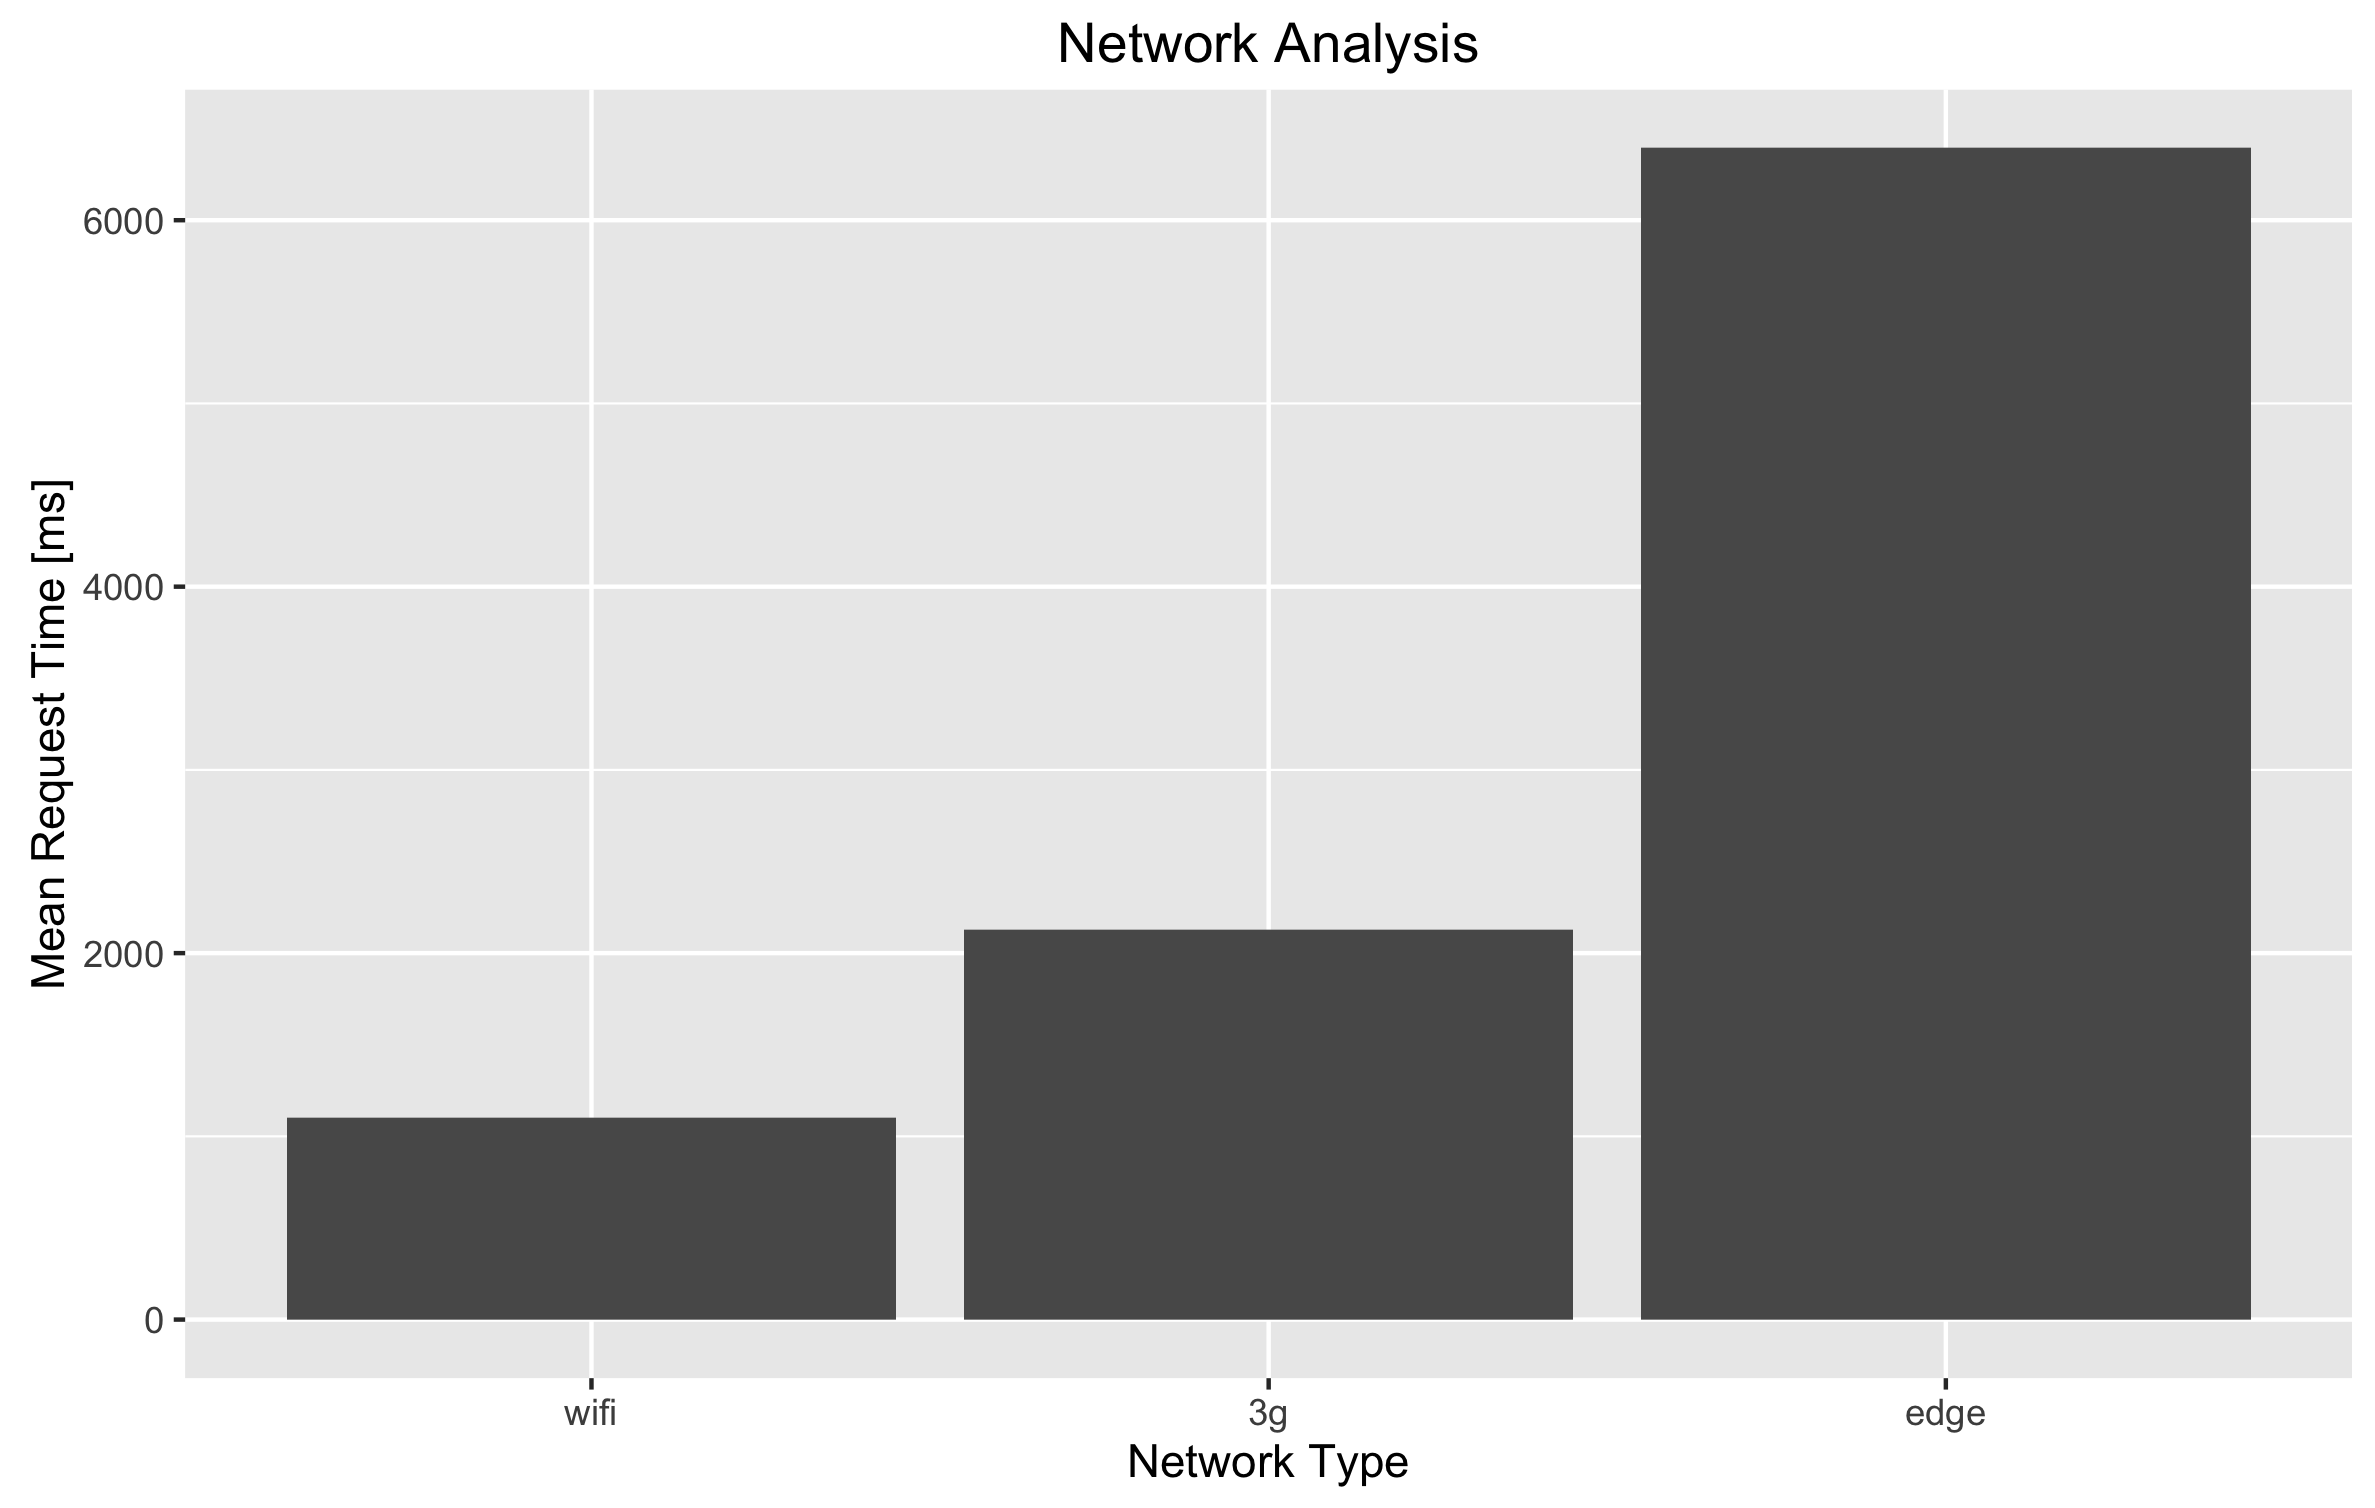
\includegraphics[width=\textwidth]{7-performance/Immagini/network_time_analysis.png}
	\caption{Analisi dei tempi di risposta con reti diverse}\label{fig:network-time-analysis}
\end{figure}


\chapter{Conclusioni e sviluppi futuri\label{ch:conclusioni}}

Questa tesi è mirata alla definizione di una metodologia valida per diversi ambiti in grado di permettere una personalizzazione dei dati ricercati dagli utenti in base alla situazione di utilizzo.

Si è focalizzata molto l'attenzione sul \emph{contesto}, a partire dai modelli che potevano essere utilizzati. Si è dimostrato come una rappresentazione ad albero permetta una definizione molto completa e semplice delle possibili situazioni nelle quali ci si può trovare. In seguito si è analizzato il problema della ricerca delle migliori fonti dalle quali acquisire informazioni. In particolare è stato proposto un metodo di associazione dei servizi al contesto mediante delle semplici regole, che permettono di selezionare solamente quelli più idonei in una particolare situazione. Si è potuto constatare come l'utilizzo del contesto permetta di avere a disposizione una quantità ottimale di informazioni per poter prendere la decisione sia per quanto riguarda i servizi da interrogare sia, una volta ricevuti i dati, per filtrarli ulteriormente e fornire così risultati ancora migliori e mirati.

L'utilizzo del contesto è complementare all'uso dei \emph{mashup}, in quanto questi ultimi permettono di definire uno schema dinamico di generazione delle applicazioni mobili che faccia uso di informazioni di supporto per arricchire i dati principali ricevuti dall'utente. Come è stato sottolineato più volte nella tesi, l'utilizzo di uno schema per la definizione della struttura dell'\emph{app} permette di ottenere vantaggi sia per quanto riguarda la flessibilità di modifica in base alla situazione di utilizzo, sia per quanto riguarda l'associazione dei servizi di supporto.

Infine si è potuta valorizzare la figura dell'\emph{esperto di settore}, che con la sua conoscenza per la progettazione delle \emph{app} permette di aiutare l'utente nella personalizzazione delle \emph{CAMUS app}. Alcune operazioni non sono automatizzabili ed è stato quindi necessario introdurre una figura umana che svolgesse determinati compiti, e gli strumenti in grado supportarle.

Si può affermare che CAMUS è un progetto molto innovativo. Dalla descrizione delle soluzioni concorrenti della Sezione \ref{sec:stato-arte} si è potuto constatare come esistano diverse soluzioni, alcune volte anche migliori di CAMUS, ma che si focalizzano su uno solo degli aspetti trattati nel progetto. CAMUS è destinato a crescere, cercando di inglobare le migliorie necessarie affinché diventi una soluzione sempre più efficace e sofisticata.

Con questa tesi si sono volute creare della basi solide per il \emph{framework}. Fornire un'esperienza per l'utente semplice ma allo stesso tempo completa non è un'operazione semplice. In particolare l'ostacolo principale riguarda l'acquisizione dei dati, in quanto esistono una varietà infinita di fonti che possono essere interrogate. Inoltre ognuna di esse possiede i propri requisiti, che variano anche in maniera marcata tra una fonte e l'altra. Nello sviluppo della tesi, dopo una risoluzione delle problematiche di maggiore rilevanza, si è data priorità allo sviluppo di alcune funzionalità \emph{core}, alcune volte in versione semplificata, in modo da fornire un punto di partenza stabile da poter espandere e migliorare. Nella prossima sezione verranno esposti alcuni punti per migliorare la soluzione presentata in questa tesi.

\section{Sviluppi futuri}

In questa sezione si vogliono esporre alcuni punti di miglioramento alle soluzioni proposte da questa tesi:

\begin{itemize}
	\item
	Si vuole lasciare più flessibilità di associazione degli \emph{alberi di contesto} e dei \emph{mashup} con gli utenti. Per quanto riguarda l'albero di contesto, una scelta può essere quella di dare una \emph{validità temporale} al CDT, in modo che venga mostrato all'utente solo in quella finestra. Può essere utile quando un utente è in viaggio e necessita spesso di cambi radicali di contesto. Per i \emph{mashup} invece si può prevedere un meccanismo di selezione basato sempre sul \emph{contesto}. Questa soluzione permetterebbe di selezionare in ogni situazione lo schema più idoneo, visto che non sarebbe più legato all'utente. Grossi vantaggi derivanti da questa scelta sono per esempio relativi alla selezione dei servizi di supporto locali, in quanto verrebbe generato un schema associato ad una particolare località e tale schema verrebbe scelto a \emph{runtime} dall'algoritmo come migliore per il luogo dove si trova l'utente
	\item
	Nella tesi, per la selezione dei nodi valori dell'albero di contesto, è stata adottata la regola che è possibile selezionare al massimo uno tra i nodi figli dello stesso nodo dimensione. Un'assunzione alla base di questa scelta è che i vari contesti siano tra loro disgiunti. \upe anche vero che non in tutti i casi quest'ultima ipotesi è verificata e questa regola risulta essere limitante nell'espressione del contesto. Un esempio riguarda la scelta dei ristoranti: si ipotizzi che un utente voglia cercare un ristorante sia per pranzo che per cena. Sarebbe sensato lasciargli la possibilità di selezionare entrambe le opzioni in modo che l'app possa fornire, se disponibili, gli orari nei quali può prenotare un tavolo
	\item 
	Al momento la risoluzione dei conflitti tra le dimensioni viene data in carico all'\emph{esperto di settore}, che si occupa di ridefinire i contesti per gli utenti. In alcuni casi però una soluzione automatica e globale sarebbe più indicata. Per esempio, non si vuole permettere all'utente di selezionare contemporaneamente come \emph{Interest Topic} \virgolette{Musei} e un qualsiasi valore della dimensione \virgolette{Tipologia Ristorante}. Come è possibile notare, il fulcro di queste associazioni è la categoria, che nel modello del contesto viene definita dagli \emph{Interest Topic}. A tal proposito è in corso di valutazione l'introduzione di un attributo \virgolette{relatedTo}, da associare ad ogni nodo dimensione del contesto, per definire a quale categoria specifica quella dimensione fa riferimento. Questo attributo è utilizzabile a discrezione dell'esperto: se ad una dimensione non viene associata nessuna categoria particolare significa che è valida per tutte quante
	\item
	Sono stati spesso citati i \virgolette{termini}, elementi necessari per permettere la conversione di una risposta dal formato specifico del servizio a quello CAMUS. Non si è mai parlato invece di come vengono organizzati questi termini. Questo è uno dei punti aperti del progetto, per il quale sono state formulate diverse ipotesi. Quella più rilevante riguarda l'utilizzo di un'\emph{ontologia} come struttura per i termini. In questo modo verrebbe arricchito il significato semantico di ogni attributo. Le ontologie mettono inoltre a disposizione una complessa rete di connessioni tra i vari elementi che la compongono. Questa caratteristica garantisce un'enorme flessibilità per l'implementazione delle funzionalità, in quanto permette di definire globalmente il significato di ogni attributo e le relazioni che possiede con le altre entità
	\item
	Nel prototipo è stata data larga importanza all'integrazione dell'\emph{app} CAMUS con il sistema operativo e le altre \emph{app} presenti sul dispositivo. Viene inoltre data la possibilità di utilizzare dei servizi di supporto invocabili tramite URL. L'utilità è quella di permettere l'aggiunta di informazioni utili per l'utente. Per esempio, se è stato scelto di utilizzare i mezzi pubblici per spostarsi sarebbe utile mostrare un'indicazione del tempo necessario per raggiungere il luogo desiderato. Questa attività può essere svolta tramite un'interrogazione verso il gestore dei trasporti pubblici per acquisirne una stima. La scelta del servizio, come è facilmente intuibile, deve variare in base alla città in cui ci si trova e ad altri fattori. L'obiettivo è la creazione di componenti che accettino informazioni da diversi servizi. Il problema che si pone è molto simile a quello dei servizi primari: ogni servizio fornisce risposte descritte in modo diverso. \upe necessario dunque creare una soluzione per certi versi simile alla trasformazione delle risposte per i servizi primari, in modo che la \emph{view} dell'\emph{app} che deve visualizzarli sia in grado di leggere i dati ricevuti
	\item
	Un’ulteriore attività del \emph{Response Aggregator}, che non è ancora stata implementata, riguarda l’assegnazione di un punteggio a ogni elemento, in base alle informazioni di contesto disponibili. Per esempio, sarà possibile assegnare un punteggio più alto all’elemento che si trova più vicino rispetto all’utente e, per gli altri elementi, verrà assegnato un punteggio che varia in modo inversamente proporzionale alla distanza dal punto di riferimento. Si stanno prendendo in considerazione anche logiche di selezione \emph{fuzzy} per permettere una flessibilità maggiore nell’assegnazione dei vari punteggi
	\item
	La \emph{mobile app} di per sè permette un'interazione molto semplice con l'utente, grazie anche al ridotto numero di schermate che gli vengono mostrate. Un eventuale punto di miglioramento riguarda uno studio sulla qualità della soluzione proposta. Si può svolgere un \emph{sondaggio} basato su un campione di utenti per valutare l'efficacia della soluzione implementata e per raccogliere suggerimenti su come migliorarla ulteriormente
	\item
	Un problema estremamente complesso, che è stato risolto solo in parte con il prototipo, riguarda le \emph{traduzioni} dei parametri nel formato accettato dal servizio. Nell'implementazione corrente viene utilizzato un sistema di traduzione di tipo chiave-valore che permette di acquisire un'informazione dal contesto e trasformarla nel valore accettato in ingresso dal servizio. I dati da tradurre però sono di tipologie estremamente diverse tra loro. Un problema comune è quello della definizione della dimensione \virgolette{Orario}, composta da \virgolette{Mattina}, \virgolette{Pomeriggio} e \virgolette{Sera}. La maggior parte dei servizi accetta un numero o un intervallo numerico. Da qui nasce l'esigenza di un sistema per effettuare questa trasformazione. La difficoltà risiede nella variabilità di questi intervalli. Non è detto che in tutte le parti del mondo si ceni alla stessa ora. Un altro esempio è il caso della dimensione \virgolette{Budget}. Per definire un budget vengono utilizzati i valori \virgolette{Basso}, \virgolette{Medio} e \virgolette{Alto}. In questo caso la difficoltà sta nel definire cosa si intende per budget: di sicuro un budget basso per un ristorante è diverso da quello di un hotel
	\item
	Nel prototipo è stato implementato unicamente il \emph{bridge} relativo ai servizi di tipo REST. Questa scelta è dettata dal fatto che la maggior parte dei servizi è interrogabile tramite questo protocollo. Un'utile aggiunta può essere l'implementazione di \emph{bridge} per altri protocolli, come per esempio SOAP. \upe conveniente utilizzare diverse implementazioni generiche in quanto un \emph{bridge}, oltre alla logica di interrogazione e composizione degli indirizzi, deve gestire anche la paginazione dei dati
	\item
	Nel prototipo è stato introdotto un sistema base per l'autenticazione degli utenti. Il motivo della sua semplicità è a causa della prevista integrazione con servizi più flessibili e sicuri. \upe stata valutata l'integrazione con \emph{Passportjs}\footnote{Passportjs: \url{http://passportjs.org/}}, un \emph{middleware} per Node.js che si occupa di autenticazione degli utenti. La sua caratteristica principale riguarda le \emph{strategie}, ovvero quale \emph{provider} di autenticazione utilizzare. In questo modo è possibile fornire all'utente la possibilità di autenticarsi anche con i propri dati di accesso a Facebook o Google
	\item
	La \emph{mobile app} al momento supporta solo una lingua. Sarà necessaria l'in\-tro\-du\-zio\-ne di un sistema che permetta di tradurre i testi nelle diverse lingue che si desidera supportare, per fornire un'interazione migliore con l'\emph{app} anche alle persone che non conoscono l'inglese. Inoltre sarà preferibile introdurre un metodo di selezione della lingua anche per i servizi che supportano questa scelta. In questo modo potranno essere recuperate le descrizioni riguardo le entità nella lingua più familiare all'utente
	\item
	Nella Sezione \ref{sec:integrazione-dati} si è parlato dell'ottimizzazione dell'algoritmo di ricerca delle entità duplicate. La tecnica utilizzata è solo una tra le tante disponibili. \upe possibile tentare con approcci di tipo \emph{machine learning} per far sì che il software impari di volta in volta a riconoscere gli elementi duplicati, ottenendo un tasso di riconoscimento migliore rispetto a quello attuale
\end{itemize}

\bibliographystyle{ieeetr}
\bibliography{bibliografia}
\addcontentsline{toc}{chapter}{Bibliografia}

\cleardoublepage{}
\end{document}
